% ---------------------------------------------------------------------------------------------------------------
% TEMPLATE PARA TRABALHO DE CONCLUSÃO DE CURSO
% Universidade Tecnológica Federal do Paraná - UTFPR
% Customização da classe abnTeX2 (http://www.abntex.net.br/) para as normas da UTFPR
%
% Projeto hospedado em: <link git>
% Autores: Diego Marczal  <>
% 	   Michael Vornes <https://github.com/mvornes>
%
%----------------------------------------------------------------------------------------------------------------
% Codificação: UTF-8
% LaTeX:  abnTeX2          
% ---------------------------------------------------------------------------------------------------------------

% CARREGA CLASSE PERSONALIZADA DA UTFPR--------------------------------------------------------------------------
\documentclass[%twoside,                   % Impressão em frente e verso
    	        oneside,                   % Impressão apenas frente
]{configuracoes/utfpr-abntex2}


% INCLUI ARQUIVOS DE CONFIGURAÇÕES-------------------------------------------------------------------------------
% REFERÊNCIAS------------------------------------------------------------------
\usepackage[%
      alf,
      abnt-emphasize=bf,
      bibjustif,
      recuo=0cm,
      abnt-url-package=url,       % Utiliza o pacote url
      abnt-refinfo=yes,           % Utiliza o estilo bibliográfico abnt-refinfo
      abnt-etal-cite=3,
      abnt-etal-list=3,
      abnt-thesis-year=final,
      num
]{abntex2cite}                  % Configura as citações bibliográficas conforme a norma ABNT
%\usepackage[num]{abntex2cite}
%\citebrackets[]

% PACOTES----------------------------------------------------------------------
\usepackage[utf8]{inputenc}                                 % Codificação do documento
\usepackage[T1]{fontenc}                                    % Seleção de código de fonte
\usepackage{booktabs}                                       % Réguas horizontais em tabelas
% \usepackage{color, colortbl}                                % Controle das cores
\usepackage[dvipsnames]{xcolor}				    % Cores predefinidas
% comentado porque inclui o pacote floatrow
% \usepackage{float}                                          % Necessário para tabelas/figuras em ambiente multi-colunas
\usepackage{graphicx}
		% Inclusão de gráficos e figuras
\usepackage{icomma}                                         % Uso de vírgulas em expressões matemáticas
\usepackage{indentfirst}                                    % Indenta o primeiro parágrafo de cada seção
\usepackage{microtype}                                      % Melhora a justificação do documento
\usepackage{multirow, array}                                % Permite tabelas com múltiplas linhas e colunas
\usepackage{subeqnarray}                                    % Permite subnumeração de equações
\usepackage{lastpage}                                       % Para encontrar última página do documento
\usepackage{verbatim}                                       % Permite apresentar texto tal como escrito no documento, ainda que sejam comandos Latex
\usepackage{amsfonts, amssymb, amsmath}                     % Fontes e símbolos matemáticos
\usepackage[linesnumbered,boxed,ruled,algoruled,portuguese]{algorithm2e}             % Permite escrever algoritmos em português
%\usepackage[scaled]{helvet}                                % Usa a fonte Helvetica
% \usepackage{times}                                          % Usa a fonte Times
%\usepackage{palatino}                                      % Usa a fonte Palatino
\usepackage{lmodern}                                       % Usa a fonte Latin Modern
\usepackage[bottom]{footmisc}                               % Mantém as notas de rodapé sempre na mesma posição
% \usepackage{ae, aecompl}                                    % Fontes de alta qualidade
\usepackage{latexsym}                                       % Símbolos matemáticos
\usepackage{lscape}                                         % Permite páginas em modo "paisagem"
\usepackage[bottom=3.25cm,marginparwidth=2cm,marginparsep=0.5cm]{geometry}
\usepackage{marginnote}                                     % Permite anotações nas margens
%\usepackage{picinpar}                                      % Dispor imagens em parágrafos
%\usepackage{scalefnt}                                      % Permite redimensionar tamanho da fonte
% \let\newfloat\undefined
% \usepackage{floatrow}                                       %
\usepackage{subfig}                                        % Posicionamento de figuras
%\usepackage{upgreek}                                       % Fonte letras gregas
\usepackage{mathtools}
\usepackage{amsthm}
% Redefine a fonte para uma fonte similar a Arial (fonte Helvetica)
\renewcommand*\familydefault{\sfdefault}

\usepackage{caption} %opçoes para formatar as captions das figuras e tabelas
\newcommand{\definicoes}[1]{
	\reversemarginpar
	\marginnote{
		\centering
		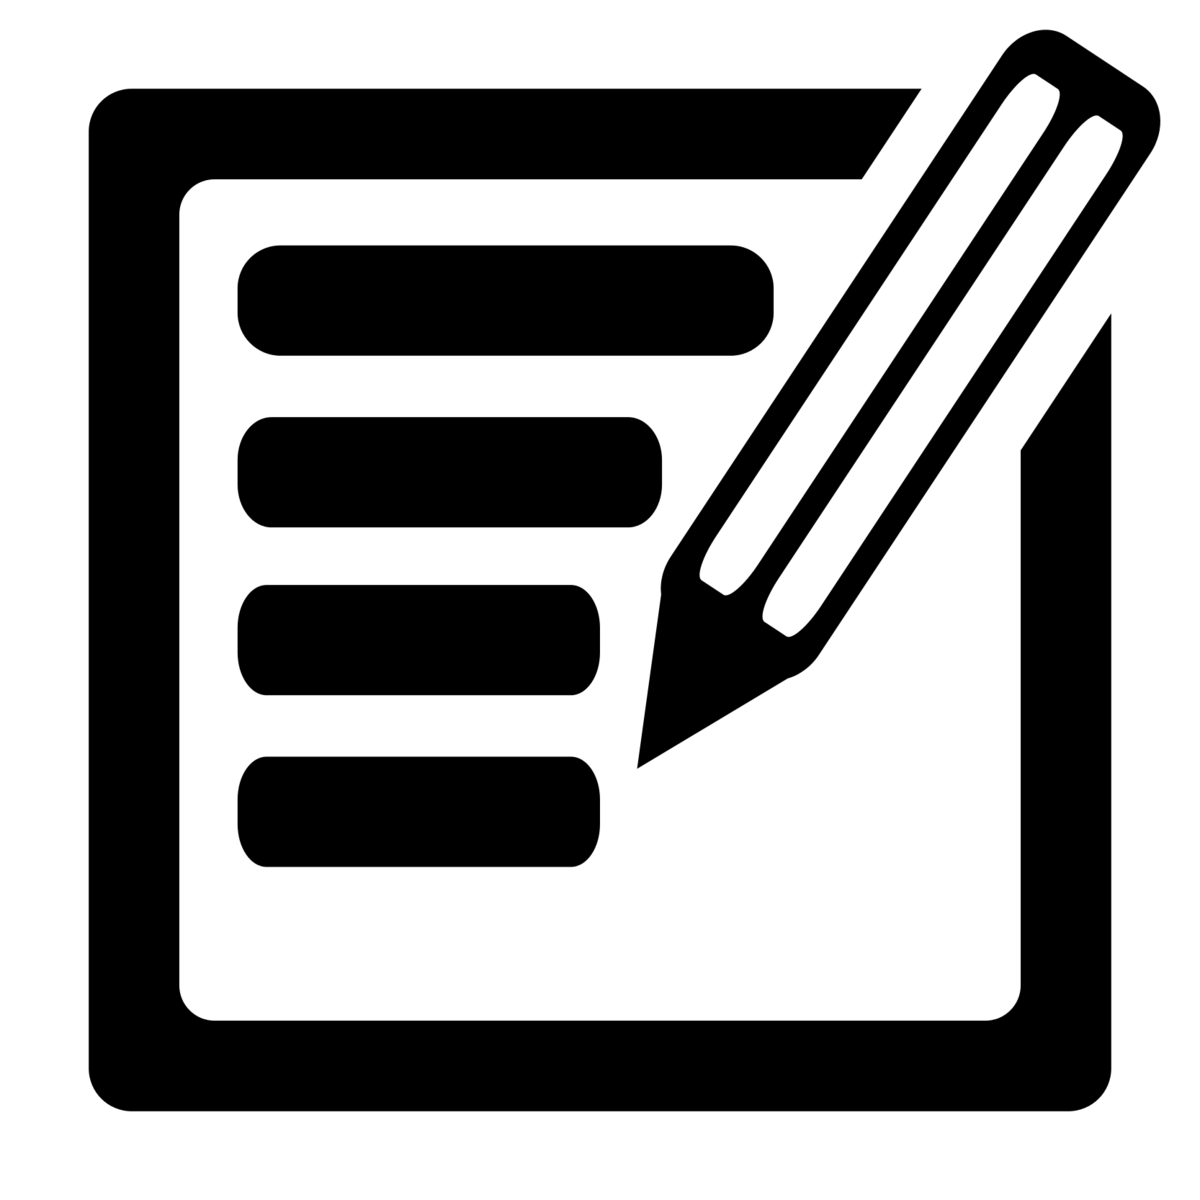
\includegraphics[scale=0.02]{dados/figuras/icone-definicao.png} \\
		\tiny #1
	}[0cm]
}

\DeclarePairedDelimiter\abs{\lvert}{\rvert}

\newcommand{\algstat}[1]{$\mathrm{#1}$}
% CONFIGURAÇÕES DE APARÊNCIA DO PDF FINAL--------------------------------------
\makeatletter
\hypersetup{%
    portuguese,
    colorlinks=true,   % true: "links" coloridos; false: "links" em caixas de texto
    linkcolor=blue,    % Define cor dos "links" internos
    citecolor=blue,    % Define cor dos "links" para as referências bibliográficas
    filecolor=blue,    % Define cor dos "links" para arquivos
    urlcolor=blue,     % Define a cor dos "hiperlinks"
    breaklinks=true,
    pdftitle={\@title},
    pdfauthor={\@author},
    pdfkeywords={abnt, latex, abntex, abntex2}
}
\makeatother

% ALTERA O ASPECTO DA COR AZUL--------------------------------------------------
\definecolor{blue}{RGB}{41,5,195}

% REDEFINIÇÃO DE LABELS---------------------------------------------------------
\renewcommand{\algorithmautorefname}{Algoritmo}
\def\equationautorefname~#1\null{Equa\c c\~ao~(#1)\null}

% CRIA ÍNDICE REMISSIVO---------------------------------------------------------
\makeindex

% HIFENIZAÇÃO DE PALAVRAS QUE NÃO ESTÃO NO DICIONÁRIO---------------------------
\hyphenation{%
    qua-dros-cha-ve
    Kat-sa-gge-los
}


% INCLUI ARQUIVOS DO TRABALHO DE CONCLUSÃO DE CURSO (PRÉ-TEXTUAIS, TEXTUAIS, PÓS-TEXTUAIS)-----------------------

% INSERE CAPA E FOLHA DE ROSTO
% CAPA---------------------------------------------------------------------------------------------------

% ORIENTAÇÕES GERAIS-------------------------------------------------------------------------------------
% Caso algum dos campos não se aplique ao seu trabalho, como por exemplo,
% se não houve coorientador, apenas deixe vazio.
% Exemplos: 
% \coorientador{}
% \departamento{}

% DADOS DO TRABALHO--------------------------------------------------------------------------------------
\titulo{Análise Comparativa de Assinaturas Digitais para Vídeos}
\titleabstract{Comparative Analysis of Digital Video Fingerprinting}
\autor{Jordy Jackson Antunes da Rocha \\
		Julia Ulson Tretel \\
		Rodrigo Machado 
}
\autorcitacao{Rocha, J. J. A, Tretel, J. U, Machado, R.} % Sobrenome em maiúsculo
\local{Curitiba}
\data{2018}

% NATUREZA DO TRABALHO-----------------------------------------------------------------------------------
% Opções: 
% - Trabalho de Conclusão de Curso (se for Graduação)
% - Dissertação (se for Mestrado)
% - Tese (se for Doutorado)
% - Projeto de Qualificação (se for Mestrado ou Doutorado)
\projeto{Trabalho de Conclusão de Curso}

% TÍTULO ACADÊMICO---------------------------------------------------------------------------------------
% Opções:
% - Bacharel ou Tecnólogo (Se a natureza for Trabalho de Conclusão de Curso)
% - Mestre (Se a natureza for Dissertação)
% - Doutor (Se a natureza for Tese)
% - Mestre ou Doutor (Se a natureza for Projeto de Qualificação)
\tituloAcademico{Bacharel}

% ÁREA DE CONCENTRAÇÃO E LINHA DE PESQUISA---------------------------------------------------------------
% Se a natureza for Trabalho de Conclusão de Curso, deixe ambos os campos vazios
% Se for programa de Pós-graduação, indique a área de concentração e a linha de pesquisa
\areaconcentracao{}
\linhapesquisa{}

% DADOS DA INSTITUIÇÃO-----------------------------------------------------------------------------------
% Se a natureza for Trabalho de Conclusão de Curso, coloque o nome do curso de graduação em "programa"
% Formato para o logo da Instituição: \logoinstituicao{<escala>}{<caminho/nome do arquivo>}
\instituicao{Universidade Tecnológica Federal do Paraná}
\departamento{DAINF - Departamento Acadêmico de Informática}
\programa{Bacharelado em Sistemas de Informação}
\logoinstituicao{0.2}{dados/figuras/logo-instituicao.png} 

% DADOS DOS ORIENTADORES---------------------------------------------------------------------------------
\orientador{Prof. Dr. Ricardo Dutra da Silva}
%\orientador[Orientadora:]{Nome da orientadora}
% \instOrientador{Universidade Tecnológica Federal do Paraná}

\coorientador[Orientador: ]{Prof. Dr. Rodrigo Minetto}
%\coorientador[Coorientadora:]{Nome da coorientadora}
%\instCoorientador{Universidade Tecnológica Federal do Paraná}

% FOLHA DE ROSTO--------------------------------------------------------------------------------------------------------

% TRABALHO DE CONCLUSÃO DE CURSO
 \preambulo{{\imprimirprojeto} apresentado ao curso de {\imprimirprograma} da {\imprimirinstituicao}, como requisito parcial para a obtenção do título de {\imprimirtituloAcademico}.}

% DISSERTAÇÃO DE MESTRADO
% \preambulo{{\imprimirprojeto} apresentada ao Programa de \mbox{Pós-graduação} da {\imprimirinstituicao}, como requisito parcial para obtenção do título de {\imprimirtituloAcademico}.}

% TESE DE DOUTORADO
% \preambulo{{\imprimirprojeto} apresentada ao Programa de \mbox{Pós-graduação} da {\imprimirinstituicao}, como requisito parcial para a obtenção do título de {\imprimirtituloAcademico}.}

% PROJETO DE QUALIFICAÇÃO DE MESTRADO OU DOUTORADO
%\preambulo{{\imprimirprojeto} apresentado ao Programa de \mbox{Pós-graduação} da {\imprimirinstituicao}, como requisito parcial para a obtenção do título de {\imprimirtituloAcademico}.}

% OBSERVAÇÕES-----------------------------------------------------------------------------------------------------------
% Altere este arquivo APENAS comentando as linhas que não se aplicam ao tipo de trabalho acadêmico desejado.



\begin{document}

\pretextual
\imprimircapa                                               	           % Comando para imprimir Capa
\imprimirfolhaderosto{}                                     		   % Comando para imprimir Folha de rosto
%INSERE ELEMENTOS PRÉ-TEXTUAIS
%\include{estrutura/pre-textuais/dedicatoria}          			   % Dedicatória
% AGRADECIMENTOS---------------------------------------------------------------

\begin{agradecimentos}[Agradecimentos]

TODO AGRADECIMENTOS

\end{agradecimentos}
        			   % Agradecimentos
%\include{estrutura/pre-textuais/epigrafe}              			   % Epígrafe
% RESUMO--------------------------------------------------------------------------------

\begin{resumo}[RESUMO]
\begin{SingleSpacing}

% Não altere esta seção do texto--------------------------------------------------------
\imprimirautorcitacao. \imprimirtitulo. \imprimirdata. \pageref {LastPage} f. \imprimirprojeto\ – \imprimirprograma, \imprimirinstituicao. \imprimirlocal, \imprimirdata.\\
%---------------------------------------------------------------------------------------

Lorem ipsum dolor sit amet, consectetur adipiscing elit. Curabitur luctus ante nec sem pretium, vel tincidunt arcu imperdiet. Interdum et malesuada fames ac ante ipsum primis in faucibus. Donec auctor, nunc sed elementum mattis, urna ex commodo metus, nec mattis metus felis at turpis. Pellentesque tincidunt metus eros, in dapibus libero imperdiet in. Sed sit amet ipsum venenatis leo bibendum mollis eget non erat. Ut ut mauris a nisl euismod semper. Sed pharetra, dui eu tempus vulputate, neque nulla varius quam, eget consequat diam ante euismod dolor. Interdum et malesuada fames ac ante ipsum primis in faucibus. Quisque vitae tincidunt nisi, vel pulvinar nunc. Vestibulum quam neque, bibendum quis iaculis at, finibus ut neque. Maecenas tincidunt eget arcu vel aliquet. Proin non iaculis ante. Etiam blandit quam at arcu consectetur, vitae volutpat elit blandit. Nam in ornare nisi, quis egestas diam. In vestibulum mauris neque, vitae iaculis mauris tincidunt vitae. \\

\textbf{Palavras-chave}: Assinatura Digital de Vídeo, Descritor

\end{SingleSpacing}
\end{resumo}

% OBSERVAÇÕES---------------------------------------------------------------------------
% Altere o texto inserindo o Resumo do seu trabalho.
% Escolha de 3 a 5 palavras ou termos que descrevam bem o seu trabalho 

             			   % Resumo em Português
%\include{estrutura/pre-textuais/abstract}             		           % Resumo em Inglês
% \include{estrutura/pre-textuais/listas/listas-ilustracoes/lista-figuras}   % Lista de Figuras
%\include{estrutura/pre-textuais/listas/listas-ilustracoes/lista-quadros}   % Lista de Quadros
% \include{estrutura/pre-textuais/listas/lista-tabelas}         		   % Lista de Tabelas
% Lista de Figuras----------------------------------------------------------------

\pdfbookmark[0]{\listfigurename}{lof}
\listoffigures*
\cleardoublepage

% LISTA DE TABELAS-------------------------------------------------------------

\pdfbookmark[0]{\listtablename}{lot}
\listoftables*
\cleardoublepage

% LISTA DE ABREVIATURAS E SIGLAS----------------------------------------------------------

\begin{siglas}
	\item[AUC] \hspace{9pt}\textit{\textbf{A}rea \textbf{U}nder the \textbf{C}urve}
	\item[BN] \hspace{9pt}\textit{\textbf{B}atch \textbf{N}ormalization}
	\item[BOSS] \hspace{9pt}\textit{\textbf{B}reak \textbf{O}ur \textbf{S}teganographic \textbf{S}ystem}
	\item[bpp] \hspace{9pt}\textit{\textbf{b}its \textbf{p}er \textbf{p}ixel}
	\item[CNN] \hspace{9pt}\textit{\textbf{C}onvolutional \textbf{N}eural \textbf{N}etwork}
	\item[FLD] \hspace{9pt}\textit{\textbf{F}isher \textbf{L}inear \textbf{D}iscriminant}
	\item[HPF] \hspace{9pt}\textit{\textbf{H}igh-\textbf{P}ass \textbf{F}ilter}
	\item[HUGO] \hspace{9pt}\textit{\textbf{H}ighly \textbf{U}ndetectable Ste\textbf{go}}
	\item[LSB] \hspace{9pt}\textit{\textbf{L}east \textbf{S}ignificant \textbf{B}it}
	\item[MiPOD] \hspace{9pt}\textit{\textbf{Mi}nimizing the \textbf{P}ower of \textbf{O}ptimal \textbf{D}etector}
	\item[OOBe] \hspace{9pt}\textit{\textbf{O}ut-\textbf{O}f-\textbf{B}ag \textbf{e}rror}
	\item[POV] \hspace{9pt}\textit{\textbf{P}air \textbf{o}f \textbf{V}alues}
	\item[PRNG] \hspace{9pt}\textit{\textbf{P}seudo-\textbf{R}andom \textbf{N}umber \textbf{G}enerator}
	\item[ReLU] \hspace{9pt}\textit{\textbf{Re}ctified \textbf{L}inear \textbf{U}nit}
	\item[ROC] \hspace{9pt}\textit{\textbf{R}eceiving \textbf{O}perating \textbf{C}haracteristic}
	\item[SPAM] \hspace{9pt}\textit{\textbf{S}ubtractive \textbf{P}ixel \textbf{A}djacency \textbf{M}atrix}
	\item[SRM] \hspace{9pt}\textit{\textbf{S}patial \textbf{R}ich \textbf{M}odels}
	\item[STC] \hspace{9pt}\textit{\textbf{S}yndrome-\textbf{T}rellis \textbf{C}ode}
	\item[S-UNIWARD] \textit{\textbf{S}patial \textbf{Uni}versal \textbf{Wa}velet \textbf{R}elative \textbf{D}istortion}
	\item[SVM] \hspace{9pt}\textit{\textbf{S}upport \textbf{V}ector \textbf{M}achine}
	\item[TanH] \hspace{9pt}\textbf{T}angente \textbf{H}iperbólica
	\item[UNIWARD] \hspace{9pt}\textit{\textbf{Uni}versal \textbf{Wa}velet \textbf{R}elative \textbf{D}istortion}
\end{siglas}

          		   % Lista de Abreviaturas e Siglas
%\include{estrutura/pre-textuais/listas/lista-simbolos}        		   % Lista de Símbolos
%\include{estrutura/pre-textuais/listas/listas-diversas/lista-algoritmos}   % Lista de Algoritmos
% SUMÁRIO----------------------------------------------------------------------

\renewcommand{\contentsname}{Sumário}

\pdfbookmark[0]{\contentsname}{toc}
\tableofcontents*
\cleardoublepage

% OBSERVAÇÕES-------------------------------------------------------------------
% Este arquivo não precisa ser alterado, pois o sumário é gerado automaticamente.
               			   % Sumário

\textual
% INSERE ELEMENTOS TEXTUAIS
\chapter{Introdução}
\label{chap:introducao}

A cada minuto é realizado o \textit{upload} de aproximadamente 300 horas de vídeo apenas na plataforma \textit{YouTube\footnote{www.youtube.com/}}, segundo os dados da pesquisa realizada pelo site \textit{Statistic Brain\footnote{www.statisticbrain.com/youtube-statistics/}}, em 2016. É provável que essa estatística seja ainda mais expressiva atualmente, devido à popularização cada vez maior de dispositivos móveis e à democratização do acesso à internet. O \textit{YouTube} é um dos serviços de hospedagem de vídeos mais utilizados na internet, em conjunto com diversas outras empresas que oferecem serviços similares, como, por exemplo, \textit{Vimeo, Twitch, DailyMotion} e, mais recentemente o \textit{Facebook}.

% 2 Parágrafos com o problema (justificativa)
É comum que essas plataformas de compartilhamento de vídeos recebam pedidos vindos de criadores de conteúdo digital (como estúdios de cinema, cineastas independentes ou ``vloggers'') solicitando a retirada de determinados vídeos alegando o infringimento de direitos autorais. Segundo estes criadores, seus vídeos estão sendo reproduzidos parcial ou integralmente sem autorização, caracterizando uma situação de pirataria e apropriação indevida de conteúdo. 

Enquanto o número de pedidos de retirada é baixo não há grandes problemas em definir se o caso realmente se trata de uma cópia, pois um humano pode analisar o vídeo e definir se realmente se trata de um caso de plágio. Entretanto, à medida que o número de pedidos cresce, levando em conta a quantidade de \textit{uploads}, torna-se inviável a realização desse processo de forma manual, gerando um problema para as plataformas, que precisam buscar métodos automáticos de detecção de duplicatas de vídeos.

Uma das técnicas já adotadas pelas empresas de compartilhamento de vídeos é a detecção de duplicatas via áudio. Um exemplo é o serviço chamado \textit{Content ID}, da Audible Magic Corporation, que disponibiliza comercialmente uma base de dados global para verificação de conteúdos protegidos por direitos autorais \cite{audiblemagic}. Tomando por exemplo o \textit{YouTube}, um dos seus sistemas de prevenção de cópias analisa o áudio de cada vídeo enviado \cite{youtubeblog}. O áudio é então comparado com uma base de dados para verificar se aquele conteúdo está de acordo com as políticas anti-pirataria da plataforma e, caso seja encontrada alguma irregularidade, o vídeo é rejeitado e a pessoa que realizou o \textit{upload} é notificada que está infringindo os termos de uso. Essa é abordagem eficaz para casos específicos, como a reprodução ilegal de um videoclipe ou a utilização ilícita de trilhas sonoras protegidas por lei. Porém, não é totalmente satisfatória para reconhecer se o conteúdo do vídeo está sendo utilizado indevidamente, justamente por utilizar o áudio para detectar duplicatas, não o vídeo. Outra característica negativa dessa técnica é que longas-metragens normalmente têm versões dubladas para cada país onde são distribuídas, aumentando o problema para detectar cópias.

%Existem serviços comerciais destinados a encontrar, de maneira automática, produções que infringem os direitos autorais. Um dos mais utilizados é o \textit{Content ID} da Audible Magic. O método utilizado cria uma assinatura baseanda no aúdio de uma mídia digital (podendo então ser utilizado tanto para vídeos, quanto para músicas), e disponibiliza um banco de dados global de assinaturas de conteúdos protegidos por propriedade intelectual. Este serviço é usado por grandes corporações como Facebook, SoundCloud e Vimeo, de acordo com  \citeauthor{audiblemagic}.

O problema de detecção de duplicatas se torna mais complexo quando os piratas utilizam técnicas de modificação nos vídeos, também conhecidas como ataques, fazendo com que sistemas de identificação mais especializados sejam necessários. Essas modificações podem ser sutis, como a remoção de alguns quadros do vídeo ou a alteração do formato de compressão, ou mais agressivas, como a modificação das cores, espelhamento, rotação e inserção de bordas nos vídeos. O desafio, entretanto, é que devido à natureza de cada ataque, pode se fazer necessária a utilização de diferentes formas de análise, já que um sistema para identificar um ataque de rotação pode ter dificuldade em detectar um ataque de remoção de quadros, por exemplo. 

Como uma possível solução complementar para esse problema, propomos um estudo sete algoritmos para identificar um vídeo em relação ao seu conteúdo \cite{hua2004robust}, \cite{lee2008robust}, \cite{cook2011efficient}, \cite{mao2015sceneframe}, \cite{kim2014rotation}, \cite{Dutta2013}, \cite{minetto2007reliable}. Essa identificação é feita através da extração de uma assinatura do vídeo, que deve ser robusta aos ataques mais comuns que um vídeo pode sofrer. O processo de produção das assinaturas varia de acordo com o algoritmo utilizado e as assinaturas são basicamente características locais, globais, espaciais ou temporais dos vídeos. 




%Nas próximas seções estão definidos conceitos utilizados neste trabalho, como quadro (\textit{frame}), vídeo e tomada, além da definição de assinatura de vídeo e algumas características consideradas importantes para a geração destas. Na seção \ref{sec:estadodaarte} são abordados os avanços no campo de detecção de cópias baseada em conteúdo.


    
    
%Para atacar esse problema, propomos a criação de uma base de dados de assinaturas de vídeos, ou \textit{fingerprints}, através da utilização de algoritmos que têm a capacidade de detectar o conteúdo do vídeo e gerar essa assinatura para representá-lo. Com a base de assinaturas, então, será possível comparará-las para identificar se existem assinaturas que são semelhantes o suficiente para afirmar se são cópias de outros vídeos ou não, ou identificar se existe alguma assinatura representando algum vídeo marcado para remoção devido aos direitos autorais.

% 1 Parágrafo de contextualização
%A Detecção de Cópias Baseada em Conteúdo é um método utilizado para a proteção de propriedade intelectual de mídias digitais, que consiste em extrair uma assinatura da mídia original e de uma mídia de teste e compará-las para identificar se as duas mídias têm o mesmo conteúdo ou não. Essa abordagem assume que a mídia contenha alguma informação única que possa ser utilizada para identificar uma cópia \citeauthor{kim2005spatiotemporal}. 

% Devemos incluir outros problemas?
% - identificação de conteúdo sendo reproduzido na TV/contar quantidade de exibições de uma propaganda
% - identificar e parar a disseminação de conteúdo proibido/impróprio




% Para combater o problema, foram propostos métodos que utilizam informações contidas nos quadros dos vídeos para a geração das assinaturas. Este trabalho propõe-se a fazer uma revisão da literatura de métodos para Detecção de Cópias Baseada em Conteúdo, selecionar seis candidatos que possuam abordagens distintas, compará-los e avaliar quais atributos do conteúdo digital devem ser escolhidos a fim de otimizar a acurácia na detecção de cópias. 

% Explicar critérios de escolha - Local, global, espacial, temporal
% Falar da organização do trabalho 

\section{Objetivo Geral}
\label{sec:objetivos}
Este trabalho tem como objetivo comparar descritores para assinatura digital de vídeos, e investigar a complementaridade de descritores espaciais em conjunto com uma proposta de descritor temporal.

\section{Objetivos Específicos}

Implementar sete algoritmos para gerar assinaturas digitais de vídeos. Criar um repositório com 1265 vídeos que sofrerão 14 tipos de ataques diferentes para testar a robustez dos algoritmos. As assinaturas dos vídeos e suas respectivas duplicadas serão registradas em  uma base de dados, que possibilitará a análise e extração de informações sobre a eficiência de cada método. %Por fim, comparar os algoritmos com base na semelhança das assinaturas e contrastar os métodos de comparação utilizados.

Parte do estudo será criar um repositório com 1265 vídeos que sofrerão 14 tipos de ataques diferentes para testar a robustez dos algoritmos. As assinaturas dos vídeos e suas respectivas duplicadas serão registradas em  uma base de dados, que possibilitará a análise e extração de informações sobre a eficiência de cada método.

\section{Estrutura do trabalho}
Este trabalho está estruturado como segue. No Capítulo 2 são apresentados conceitos básicos, uma introdução aos métodos de detecção de conteúdo em vídeos, os seis algoritmos selecionados para a geração de assinaturas e trabalhos relacionados. O Capítulo 3 detalha a base de vídeos utilizada, a forma como o experimento foi realizado e as métricas de comparação. No Capítulo 4 são apresentados os resultados experimentais. Finalmente, são apresentadas as conclusões do estudo e sugestões de trabalhos futuros.















                		           % Introdução
% REVISÃO DA LITERATURA--------------------------------------------------------

% \chapter{Revisão da Literatura}
% \label{chap:revisao_da_literatura}
%------------------------------------------------------------------------

\chapter{Revisão da Literatura}
\label{chap:revisao}

As Seções \ref{sec:video} à \ref{sec:ataques} apresentam definições úteis para melhor compreensão do trabalho, como vídeo e suas divisões, técnicas de detecção de cópias e conteúdo em vídeo, os principais tipos de ataques que um vídeo pode sofrer, assinatura e descritores de vídeos, que são os algoritmos utilizados para gerar assinaturas.

\section{Trabalhos relacionados}
\label{chap:relacionados}

  % Artigo 9 - 372: Ele fala de técnicas na história - comparar cenas (final/inicio): comparar descritores; - transformação pós-produção: utilização de pontos de interesse;


Em 1999, o compartilhamento de vídeos na internet ainda era uma realidade distante, entretanto, \citeauthor{indyk1999finding} já buscava métodos para encontrar vídeos pirateados e duplicatas na rede. Os autores então propuseram um algoritmo para geração de assinaturas temporais baseadas nos limites das cenas de um vídeo. Embora este método seja bom para encontrar filmes e vídeos longos, ele não é apropriado para identificar vídeos curtos e cenas isoladas, com duração de até quatro minutos. Esse tipo de produção é a mais comum nas plataformas de compartilhamento de vídeos atualmente \citeauthor{comscoreinc}.

Desde então, várias técnicas têm sido usadas para a geração de assinaturas de vídeos. \citeauthor{coskun2006spatio} propuseram o conceito de funções de \textit{hash} como uma ferramenta para identificação dos vídeos, criando um algoritmo que utiliza as informações espaço-temporais do vídeo baseado no diferencial da luminância entre regiões de quadros. Outras abordagens incluem o uso de descritores globais que utilizam a distribuição da intensidade de movimento e cor \citeauthor{hampapur2001comparison}, além de medidas ordinais \citeauthor{hua2004robust}, que se provaram robustas para variadas resoluções, mudanças de iluminação e formatos de vídeos.	   	

Descritores locais também foram extensamente pesquisadas, como em \citeauthor{joly2007content}, cujo algoritmo apresentado busca ser eficiente para buscas em grandes bases de dados, tanto em velocidade quanto em qualidade. Há também a  pesquisa de \citeauthor{law2006robust}, que usa o algoritmo de Harris para encontrar pontos de interesse no vídeo e criar uma assinatura compacta.

\citeauthor{de2012combinaccao} fez um estudo comparativo entre descritores globais e locais e mostrou como unir os dois tipos de descritores através de algoritmos genéticos. \citeauthor{de2012combinaccao} também fez vários experimentos mostrando que a combinação de descritores globais e locais são complementares e se usados em conjunto, produzem resultados superiores quando comparados com o uso individual de cada tipo de descritor.

\citeauthor{hu2011survey} discorre sobre a indexação e recuperação de conteúdo em vídeos. O trabalho apresenta métodos para analisar a estrutura de vídeos, segmentação de cenas, extração de quadros-chave, características de movimento, mineração de informações em vídeos, mensuramento de similaridade e relevância entre assinaturas digitais, pesquisa de conteúdo em vídeos entre outros.


\section{Vídeo}
\label{sec:video}  

\textbf{}	Um vídeo pode ser descrito quanto ao seu conteúdo em quatro níveis de detalhe, sendo o nível mais baixo um conjunto de quadros \citeauthor{lienhart1997video}. Um quadro (ou \textit{frame}) $I$ é uma imagem representada por uma matriz de altura $h$ e largura $w$ em que cada ponto $I[x,y]$ representa a intensidade de um \textit{pixel}. Além disso, um quadro possuí um determinado tempo, que representa o instante em que é exibido no vídeo. De maneira resumida, um vídeo é uma sequência de imagens. Normalmente são exibidas 24 imagens por segundo, sendo esse o conceito de quadros por segundo, ou FPS \textit{(frames per second)}. 

	Logo acima na hierarquia existem as tomadas, termo que se refere a um ou mais quadros capturados em sequência, representando uma ação ininterrupta no tempo e no espaço. Tomadas contínuas podem ser agrupadas em cenas para gerar coerência na história do vídeo. Um vídeo pode ser composto por uma ou mais cenas.

       Um conceito importante também relacionado a vídeo é o quadro de cena, utilizado pelo algoritmo de \citeauthor{mao2015sceneframe}, um dos descritores que fazem parte do experimento proposto. \citeauthor{7848130} definem quadro de cena como a imagem que define os pontos de início e fim de qualquer transição suave de imagens, é o quadro que melhor representa a cena no geral. Quadros de cena são amplamente utilizados na produção de animações, onde normalmente o objeto ou sujeito da imagem se move em relação ao fundo \textit{(background)}. 

	De acordo com \citeauthor{mao2015sceneframe}, o quadro de cena deve possuir todos os mesmos elementos (pessoas, objetos, animais, etc.) exibidos na cena e o background deve ser altamente similar ao restante dos quadros. Na Figura \ref{fig:quadro_cena}, qualquer um dos cinco quadros pode ser eleito como o quadro de cena, pois todos têm os mesmos elementos (a mesma pessoa e o mesmo cachorro), além do background ser praticamente o mesmo em todos os quadros.

 \begin{figure}[!htb]
      \centering
      \caption{Sequência com cinco quadros representando uma cena, retirado de um dos vídeos do repositório.}
       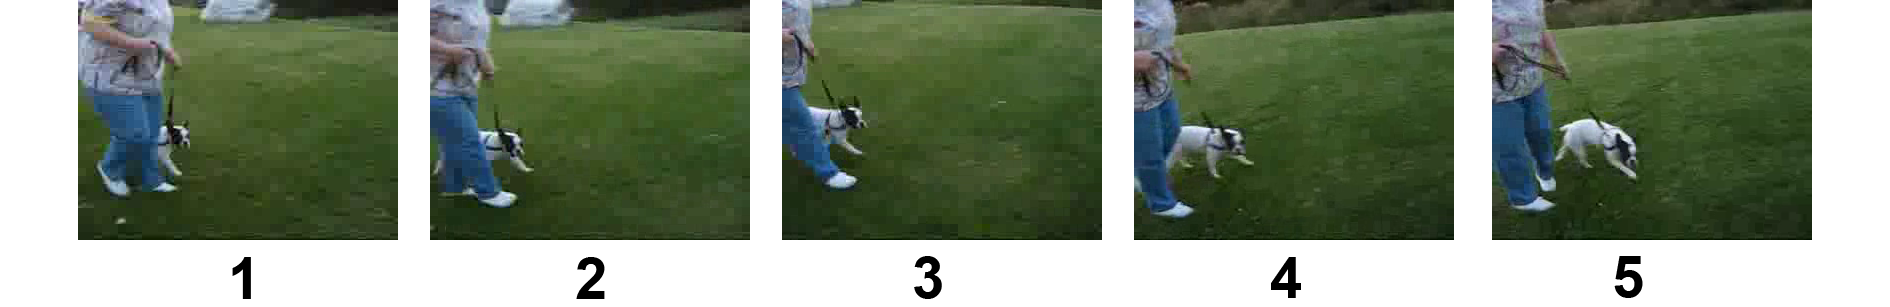
\includegraphics[width=0.96\textwidth]{dados/figuras/keyframe.png}
       \fonte{Autoria própria}
      \label{fig:quadro_cena}
    \end{figure}   
    

    
    Em um vídeo existe também a dimensão espacial e a dimensão temporal. A dimensão espacial é classificada como a distribuição e a maneira com que os elementos estão organizados em um quadro. A dimensão temporal é a relação na qual os elementos e os quadros mudam ao longo de um vídeo \citeauthor{hampapur2001comparison}.
    
\section{Transformada de Haar}

Um conceito importante para dois dos algoritmos que serão apresentados (Sub-seções  \ref{wavelets} e \ref{sec:gradientes}) é o da transformada de Haar, que consiste na separação de um sinal (ou quadro, neste caso) em 4 partes: 

\begin{enumerate}
\item $LL$, que contém $1/4$ dos dados originais, removendo os detalhes;
\item $LH$, que contém a derivada na horizontal do quadro;
\item $HL$, que contém a derivada na vertical do quadro;
\item $HH$, que contém a derivada na diagonal do quadro.
\end{enumerate}

A transformada pode ser aplicada de forma recursiva $n$ vezes, usando o quadro $I$ como entrada inicial do algoritmo e o $LL$ como entrada das chamadas subsequentes. Um exemplo do resultado da transformada de Haar pode ser visto na Figura \ref{fig:transf_haar}.

 \begin{figure}[h]
      \centering
      \caption{Sequência de recursões da transformada em uma imagem.}
      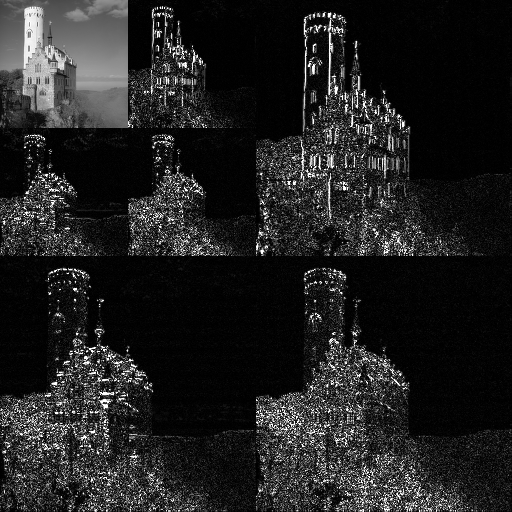
\includegraphics[width=0.96\textwidth]{dados/figuras/haar.png}      
      \fonte{Autoria própria}
      \label{fig:transf_haar}
    \end{figure}  

\section{Técnicas de detecção de cópias de vídeo} 
     
%      Existem diversas maneiras para detecção de cópias de vídeos. Foram selecionadas três delas, que são: detecção de cópias baseada em conteúdo (CBCD, do inglês \textit{Content Based Copy Detection}) \citeauthor{jiang2011pku}, recuperação de vídeo baseado em conteúdo (CBVR, \textit{Content Based Video Retrieval}) \citeauthor{law2007video} e recuperação de imagens baseada em conteúdo (CBIR, \textit{Content Based Image Retrieval}) \citeauthor{gudivada1995content}.
     
    A detecção de cópias baseada em conteúdo (CBCD, do inglês \textit{Content Based Copy Detection}) é uma técnica para identificar vídeos através da criação de uma assinatura digital baseada em seu conteúdo \citeauthor{jiang2011pku}. Apesar de o método ser utilizado em diversas aplicações a detecção de cópias torna-se um desafio, considerando que a cópia pode sofrer ataques, distorções e transformações que dificultem a identificação do vídeo por um sistema automatizado. 

%De acordo com \citeauthor{law2007video}, recuperação de vídeo baseado em conteúdo propõe algoritmos para gerar assinaturas e estudar a similaridade entre elas. É uma técnica que, através da assinatura do vídeo, permite a busca de trechos e cenas, característica que é útil para encontrar réplicas parciais de vídeos. Ainda segundo \citeauthor{law2007video}, CBVR tem foco em procurar e encontrar vídeos em uma mesma categoria, ou seja, vídeos que são similares entre si, como por exemplo, jogos de futebol, vídeos sobre balões, vídeos de pessoas tocando instrumentos musicais, etc.

%Para \citeauthor{gudivada1995content}, recuperação de imagens baseada em conteúdo, é um sistema que auxilia na recuperação e extração de imagens de acordo com o conteúdo da imagem. Para gerar uma assinatura o sistema CBIR se baseia em elementos visuais como cores, texturas e formas \citeauthor{vikhar2016improved}. Há diversas aplicações que se beneficiam desta tecnologia, como: previsão do tempo, serviços de informações geográficas, design de interiores, galerias de arte, etc \citeauthor{gudivada1995content}.
         
         
         



\section{Tipos de ataques em vídeos}
\label{sec:ataques}

	Para evitar a detecção de duplicatas é comum a realização de ataques, ou distorções, nos vídeos. Existem várias maneiras de modificar um vídeo, como redimensionamento do tamanho, inserir ou remover alguns quadros, alteração de cada quadro individualmente através da adição ou remoção de elementos.

	No escopo deste trabalho são estudados 14 tipos de ataques para simular as táticas mais comuns utilizadas pelos apropriadores de conteúdo que tentam dificultar o reconhecimento de duplicatas. Os ataques são: adição de texto e legendas no vídeo, adição de marca d'água, adição de quadro ou bordas, redimensionamento da altura e largura dos quadros, eliminação de uma faixa ou região dos quadros, inversão/espelhamento, rotação, borramento, inversão de cores, alteração do formato de compressão dos quadros do vídeo, aceleramento do vídeo e, finalmente, remoção de quadros. A Figura \ref{fig:ataques} ilustra o resultado da aplicação dos ataques acima em uma imagem.

    	\begin{figure}[h]
        \centering
         \caption{Exemplos de ataques em uma imagem.}
        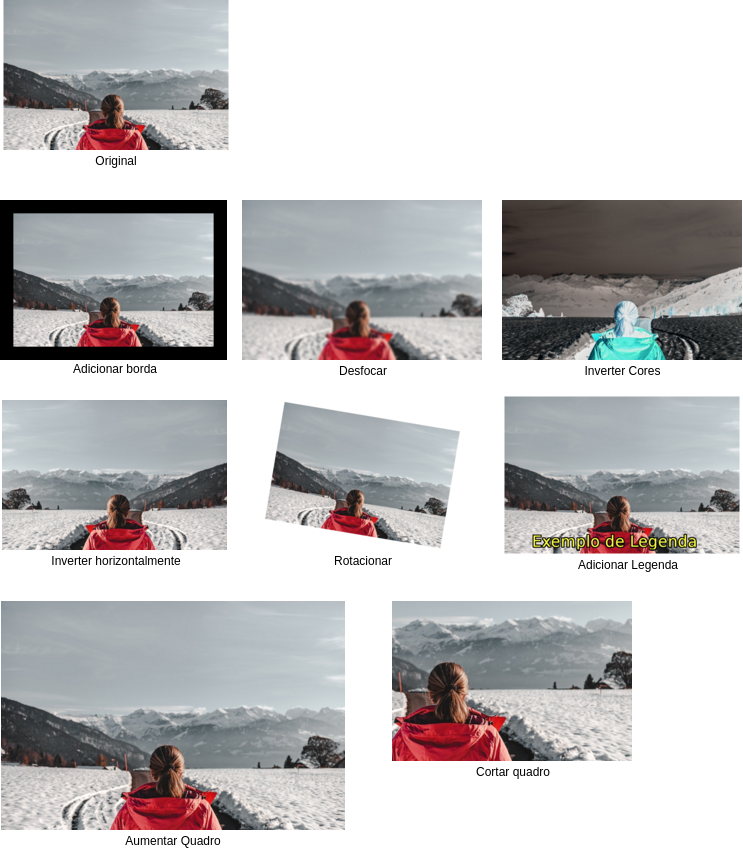
\includegraphics[width=0.8\textwidth]{dados/figuras/Ataques.png}
        \fonte{Autoria própria}
       
        
    	\label{fig:ataques}
    \end{figure}

Os ataques dos tipos remoção de quadros, alteração do formato de compressão e aceleramento do vídeo só são perceptíveis na visualização dos vídeos em um dispositivo de exibição, como um computador, e por isso não estão representados na Figura 3. O ataque do tipo remoção de quadros consiste em remover alguns quadros ao longo do vídeo e muitas vezes passa despercebida ao olho humano. O maior indicativo de que um vídeo sofreu esse ataque é observar a diferença temporal entre uma duplicata e o vídeo original, sendo que a duplicata terá uma duração menor em relação ao original. O ataque do tipo alteração da taxa de quadros também é realizado através da remoção de alguns quadros do vídeo, entretanto, o vídeo permanece com a mesma duração, pois os quadros restantes são na verdade exibidos por mais tempo, ou seja, um quadro que era exibido durante um segundo passa a ser exibido durante dois segundos. O ataque do tipo alteração do formato de compressão é ainda mais difícil de ser percebido por humanos pois em muitos casos a diferença na imagem é muito sutil e geralmente ocorre em regiões que não são o foco da atenção do observador. Uma forma de descobrir se um vídeo sofreu esse tipo de ataque é observar o tamanho em disco da duplicata em relação do vídeo original, sendo que a duplicata normalmente ocupa menos espaço em disco devido à compressão \textit{lossless} do formato JPEG.

Os ataques podem ainda ser classificados como geométricos, fotométricos ou temporais. Ataques geométricos afetam as características globais dos vídeos, ataques fotométricos as características locais e, os ataques temporais, a dimensão temporal dos vídeos. A classificação dos ataques que serão utilizados nos vídeos deste trabalho é exibida na Tabela \ref{tab-classificacao-ataques}.

\begin{table}[!ht]
\centering
\caption{Classificação de ataques em vídeo}
\label{tab-classificacao-ataques}
\begin{tabular}{|l|l|l|}
\hline
\# & \textbf{Ataque}                    & \textbf{Tipo} \\ \hline
1           & Aceleramento                       & Temporal      \\ \hline
2           & Adição de bordas                   & Fotométrico   \\ \hline
3           & Adição de texto (legendas)         & Fotométrico   \\ \hline
4           & Alteração do formato de compressão & Fotométrico   \\ \hline
5           & Borramento                         & Fotométrico   \\ \hline
6           & Eliminação de faixa ou região      & Geométrico    \\ \hline
7           & Espelhamento                       & Fotométrico   \\ \hline
8           & Inversão de cores                  & Fotométrico   \\ \hline
9           & Marca d'água                       & Fotométrico   \\ \hline
10          & Redimensionamento                  & Geométrico    \\ \hline
11          & Remoção de quadros                 & Temporal      \\ \hline
12          & Rotação                            & Geométrico    \\ \hline
\end{tabular}
\end{table}





\section{Assinaturas de vídeo}
\label{sec:assinatura} 
    
	Uma assinatura de vídeo é definida como um vetor de características que representa um vídeo e o diferencia de outros \citeauthor{lee2008robust}. Em outras palavras, a assinatura é uma representação de um vídeo em uma estrutura de dados. 
        
	Para um algoritmo de geração de assinatura ser considerado eficiente, é importante que três características sejam consideradas: robustez, singularidade e eficiência de busca. De acordo com \citeauthor{lee2008robust}, uma assinatura é considerada robusta caso o descritor gerado para um vídeo modificado seja similar ao descritor do vídeo original. A singularidade é a capacidade do algoritmo de gerar assinaturas diferentes para vídeos perceptivelmente diferentes. Por fim, eficiência de busca é a capacidade da assinatura  ser utilizada por uma aplicação para buscas em banco de dados de larga escala. Nesta monografia, são avaliadas apenas a robustez e a singularidade das assinaturas.   
    
% \textbf{[seção será complementada ou reescrita]}
% Para a geração das assinaturas, no entanto, podemos definir um vídeo quanto à estrutura de dados com a qual ele é composto. Segundo \citeauthor{simoes2004detecccao}, um vídeo é representado por uma sequência de quadros dispostos através de uma amostra temporal. Logo, faz-se necessária a definição formal de quadro, apresentada a seguir



    Existem duas classes principais de algoritmos para descrever vídeos e então gerar assinaturas, são elas: descritores locais e descritores globais. Cada classe tem características que a faz mais robusta para combater diferentes tipos de ataques, sendo então cada uma indicada para situações diferentes.
    
    Descritores locais geram assinaturas baseadas em pontos ou regiões de interesse de cada quadro do vídeo. Os pontos de interesse são determinados a partir de regiões que possuem uma acentuada variação na orientação do gradiente dos elementos presentes em um quadro, como por exemplo o enquadramento de uma porta ou o pico de uma montanha. As regiões de interesse são determinadas pelos \textit{pixels} ao redor de um ponto de interesse e ajudam a determinar os limites dessas regiões \citeauthor{radhakrishnan2007content}. Esses descritores normalmente são robustos contra variações fotométricas (borrados, iluminação, cores, ruído e compressão JPEG) e podem ser custosos computacionalmente devido aos cálculos necessários para determinar os pontos de interesse \citeauthor{naini2014vanishing}. Um descritor local consiste normalmente de três etapas: detecção das características, descrição das características e combinação das características, de acordo com \citeauthor{chen2010zernike}.

    A classe de descritores globais, ao contrário dos descritores locais, geram assinaturas utilizando informações pertinentes ao quadro como um todo, como por exemplo a luminância total do quadro. Esses podem apresentar vantagens em relação aos descritores locais, pois normalmente é menos custoso em termos computacionais trabalhar com informações gerais do quadro ao invés de realizar uma análise para determinar pontos de interesse. Além disso, os descritores globais podem gerar assinaturas mais robustas quando considerados os ataques geométricos às imagens \citeauthor{law2007video}. 
    
%==================================================================================
\section{Algoritmos para geração de assinaturas}
	A seguir é apresentado o estudo dos seis algoritmos que foram selecionados e implementados para a realização do experimento.


% --------------------------------------------------------------------------------------------------
%
% MEDIDA ORDINAL
%
% --------------------------------------------------------------------------------------------------
\subsection{Assinatura baseada na medida ordinal}
\label{sec:med_ordinal}

	O algoritmo proposto por \citeauthor{hua2004robust} baseia-se na intensidade dos \textit{pixels} de cada quadro para compor a assinatura. O que se propõe é que, primeiramente, a taxa de amostragem, ou seja, a taxa de quadros por segundo \textit{(FPS)} do vídeo de entrada seja padronizada, para que a assinatura gerada fique mais compacta e seja tolerante a diferentes formatos de compressão, por exemplo. Além disso, o vídeo é convertido para escala de cinza.

Após esse pré-processamento, para cada quadro é realizada a divisão em $M \times N$ blocos, como pode ser observado na Figura \ref{fig:medidaord}, bem como o cálculo da intensidade média para cada um dos blocos. Esses valores são então organizados em ordem crescente em um vetor representando a assinatura do vídeo.

	\begin{figure}[!htb]
        \centering
        \caption{Exemplo de divisão em blocos, cálculo das intensidades médias e ordem atribuída a cada valor.}
        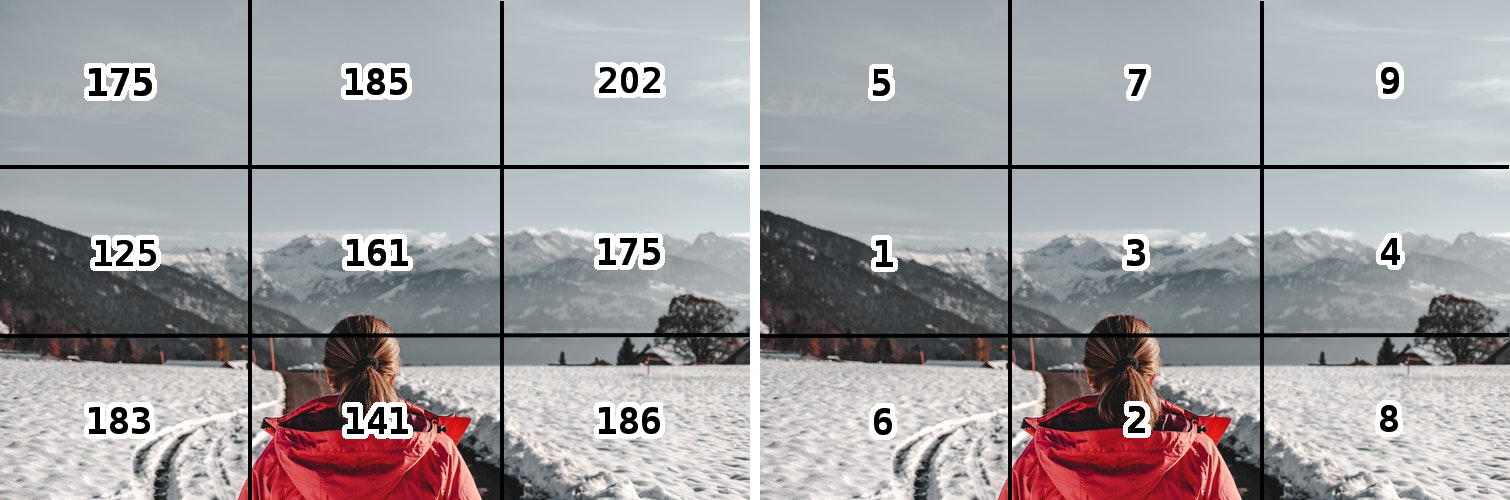
\includegraphics[width=0.8\textwidth]{dados/figuras/mo_final.png}
        \fonte{Autoria própria}
        \label{fig:medidaord}
    \end{figure}

 \begin{figure}[!htb]
      \centering
      \caption{Diagrama do algoritmo baseado em medida ordinal.}
      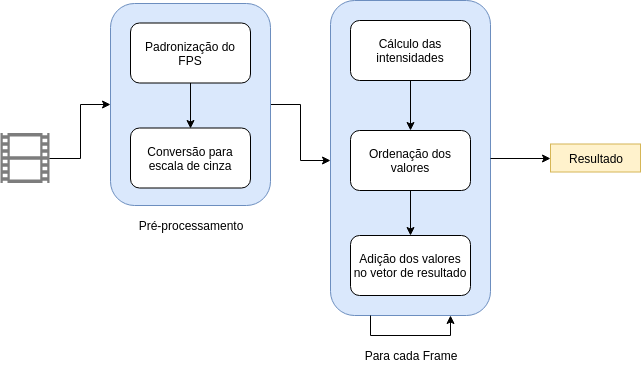
\includegraphics[width=0.96\textwidth]{dados/figuras/MedidaOrdinal.png}
      \fonte{Autoria própria}
       	\label{fig:dia_ordinal}
    \end{figure}  

% --------------------------------------------------------------------------------------------------
%
% GRADIENTE
%
% --------------------------------------------------------------------------------------------------


\subsection{Assinatura baseada em gradientes}
\label{sec:gradientes}

	O algoritmo proposto por \citeauthor{lee2008robust} utiliza a distribuição dos gradientes para geração de assinaturas. O primeiro passo é definir uma taxa de quadros por segundo (FPS) fixa, além da conversão para escala de cinza. Também é realizado o redimensionamento dos quadros, tornando o método robusto independente da mudança de resolução do vídeo. Em seguida, os gradientes $\mathbb{G}x$ e $\mathbb{G}y$ dos \textit{pixels} de cada quadro são calculados como mostra a Equação \ref{eq:gmatrix}.

\begin{equation}
  \label{eq:gmatrix}
  \begin{bmatrix}
    \mathbb{G}x
    \\ 
    \mathbb{G}y
  \end{bmatrix}= 
  \begin{bmatrix}
    \partial I/\partial x
    \\ 
    \partial I/\partial y
  \end{bmatrix}=
  \begin{bmatrix}
    \mathbb{I}(x+1, y) - \mathbb{I}(x-1,y)
    \\ 
    \mathbb{I}(x, y+1) - \mathbb{I}(x,y-1)
  \end{bmatrix}
\end{equation}
    
	O quadro é então dividido em $M\times N$ blocos, para quais é determinado o valor do centroide dos gradientes, criando assim um vetor com $(M \times N)$ elementos. Para isso, é necessário encontrar a magnitude \textit{$w(x,y)$} e a orientação \textit{$\Theta(x,y)$}, conforme mostra a Equação \ref{eq:mag-or}.
    
\begin{equation}
	\label{eq:mag-or}
    w(x,y) = \sqrt{\mathbb{G}x^{2} + \mathbb{G}y^{2}}
\qquad
\Theta(x,y) = tan^{-1}\left (\frac{\mathbb{G}y}{\mathbb{G}x} \right)
\end{equation}
    
    Em seguida o centroide para cada bloco é obtido a partir do somatório do produto da magnitude e orientação, dividido pela somatória de todas as magnitudes daquele bloco, como pode ser observado na Equação \ref{eq:gradientes}.
    
\begin{equation}
	\label{eq:gradientes}
	[i] = \frac{\sum_{x,y \in b[i]} w(x,y)\Theta (x,y)}{\sum_{x,y \in b[i]} w(x,y)}
\end{equation}

 \begin{figure}[h]
      \centering
      \caption{Diagrama do algoritmo baseado em gradientes.}
      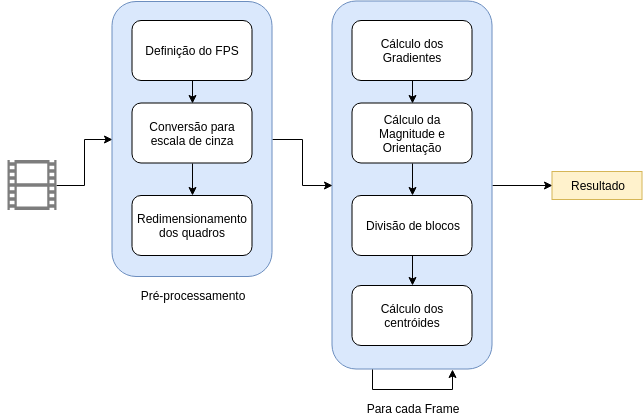
\includegraphics[width=0.96\textwidth]{dados/figuras/Gradientes.png}
      \fonte{Autoria própria}
       	\label{fig:dia_gradiente}
    \end{figure}  
    
% --------------------------------------------------------------------------------------------------
%
% FRAME DIFF
%
% --------------------------------------------------------------------------------------------------

\subsection{Assinatura baseada na diferença entre quadros}
\label{sec:framediff}

  O algoritmo proposto por \citeauthor{cook2011efficient} utiliza características globais de luminância e de diferença de luminância intra-quadros. Para cada quadro do vídeo são coletadas características primáris, como a luminância total ($Y$), obtida através da soma da luminância de todos os \textit{pixels} do quadro, a luminância máxima ($Y_{max}$), que é o valor do pixel mais brilhante do quadro e a luminância diferencial ($dY$), sendo a diferença absoluta de luminância pixel a pixel do quadro atual com o quadro que estava visível há 100 milisegundos, a diferença resultante é somada conforme mostra a equação \ref{eq:framediff}. Os valores obtidos são então normalizados, levando em conta a dimensão dos quadros do vídeo.
  
\begin{equation}
	\label{eq:framediff}
	dY = \sum_{x,y \in  \mathbb{I,J}} |\mathbb{I}(x,y) - \mathbb{J}(x,y)|
\end{equation} 

   Após a obtenção das características primárias, um filtro passa-baixa \textbf{[QUAL FILTRO? VER NO CÓDIGO]} é utilizado para suavizar a assinatura, como pode ser observado na Figura ~\ref{fig:framediff-passa-baixa}. %Além disso, duas outras características, quietude e créditos, são derivadas das características principais e visam medir o quão imóvel uma sequência de quadros é. Para isso, são definidas as medidas "Quietude" (Equação \ref{eq:framediff-stillness}) e "Créditos" (Equação \ref{eq:framediff-credits}).

%   \begin{equation}
%     \label{eq:framediff-stillness}
%     Quietude = 100 \times \left(\sqrt{\frac{\ln\frac{dY}{A}}{\ln256}}\right) \\
%   \end{equation}

%   \begin{equation}
%     \label{eq:framediff-credits}
%     Créditos = 100 \times \frac{\frac{Y_{max}}{256} + \left( 1 - \left( \frac{\ln\frac{Y}{A}}{\ln256} \right)^2\right)}{2}
%   \end{equation}


\begin{figure}[h]
\centering
	\caption{Linha azul mostra os valores originais do vetor $dY$ e a linha alaranjada mostra os valores pós filtro passa-baixa.}
  	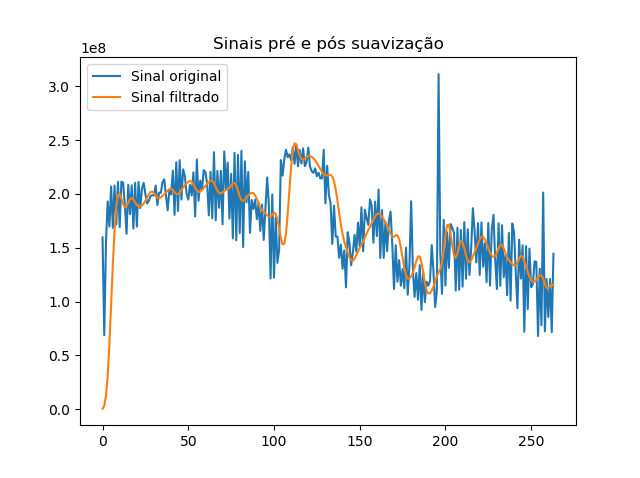
\includegraphics[width=0.7\textwidth]{dados/figuras/filtro_passa_baixa}
  	\fonte{Autoria própria}
  \label{fig:framediff-passa-baixa}
\end{figure}


A Figura \ref{fig:framediff-comparacao} mostra a característica $dY$ plotada para um vídeo original e sua versão distorcida com efeitos de borramento e adição de legenda, além de mostrar os valores de $dY$ para outro vídeo não relacionado.

\begin{figure}[h]
  \centering
  \caption{Comparação entre os vetores de característica $dY$ gerados para um vídeo, uma cópia com o efeito de desfoque, uma cópia com uma legenda inserida, e um outro vídeo qualquer.}
  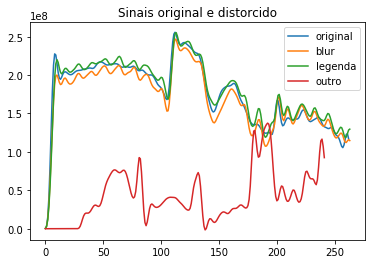
\includegraphics[width=0.7\textwidth]{dados/figuras/dy}
  \fonte{Autoria própria}
  \label{fig:framediff-comparacao}
\end{figure}


 \begin{figure}[h]
      \centering
      \caption{Diagrama do algoritmo baseado na diferença entre quadros.}
      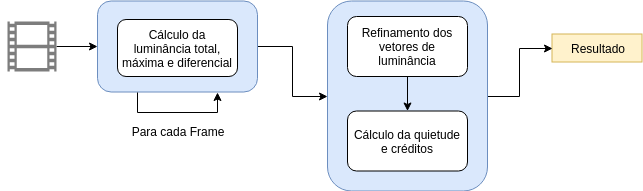
\includegraphics[width=0.96\textwidth]{dados/figuras/FrameDiff.png}
      \fonte{Autoria própria}
       	\label{fig:dia_framediff}
    \end{figure}  

%% --------------
%% TODO: explicar comparação
%% --------------

%   Dados dois quadros $\mathbb{I}$ e $\mathbb{J}$, a assinatura temporal desenvolvida por \cite{cook2011efficient} utiliza dois componentes principais para sua construção. O primeiro é a luminância total $Y$, ou seja, a soma dos \textit{pixels} do \textit{frame}, representando o brilho total da imagem. O outro parâmetro é $dY$, ou diferencial de luminância, sendo a diferença do quadro atual com o quadro anterior. $dY$ é uma métrica para saber o quanto a luminância varia com a mudança dos quadros no vídeo.  Essa variação pode acontecer, segundo o autor, a partir do movimento da câmera, corte entre cenas e objetos e pessoas que entram ou saem de cena. 
    
%    O  valor de $dY$ pode ser obtido através da Equação \ref{eq:framediff} \cite{sylvio2015}: 

% Portanto cada \textit{frame} será representando por uma tupla $(Y, dY)$.

 

% --------------------------------------------------------------------------------------------------
%
% SCENE FRAME
%
% --------------------------------------------------------------------------------------------------

\subsection{Assinatura baseada em quadros de cena}

  A abordagem proposta por \citeauthor{mao2015sceneframe} é baseada na assinatura de quadros de cena. De acordo com os autores, os quadros de cena podem ser \textit{intraframes}, ou seja, quadros que iniciam tomadas, quanto \textit{interframes}, contanto que sigam as características descritas em \ref{sec:video}, ou seja, possuir todos os mesmos elementos dos quadros restantes e o mesmo \textit{background}.

A assinatura individual de cada quadro é calculada, como pode ser observado no Diagrama \ref{fig:dia_sceneframe}. Os quadros passam por um pré-processamento, onde o componente de luminância é extraído, o quadro é recortado, mantendo-se apenas sua região central e redimensionado para o tamanho definido de $3/4$QCIF (\textit{Quarter Common Intermediate Format}, ou Formato Intermediário Comum), valor padrão utilizado para resolução de imagens, neste caso, $(108\times132)$. Além disso, é aplicado o filtro de passa-baixa da Gaussiana.

Após o processamento inicial, o quadro é então dividido em $144$ pedaços menores, de tamanho $(9\times11)$, cuja média de intensidade irá compor parte da assinatura deste quadro. Além dos $144$ valores, o descritor é composto também por $576$ elementos diferenciais, totalizando $720$ valores. Para obter esses elementos, cada fragmento é dividido em oito elementos menores, como mostra a Figura \ref{fig:divsceneframe}, e então é realizada a subtração de $a - b$, $c - d$, $e - f$ e $g - h$.

\begin{figure}[h]
  \centering
    \caption{Divisão da imagem para cálculo dos elementos diferenciais.} 
    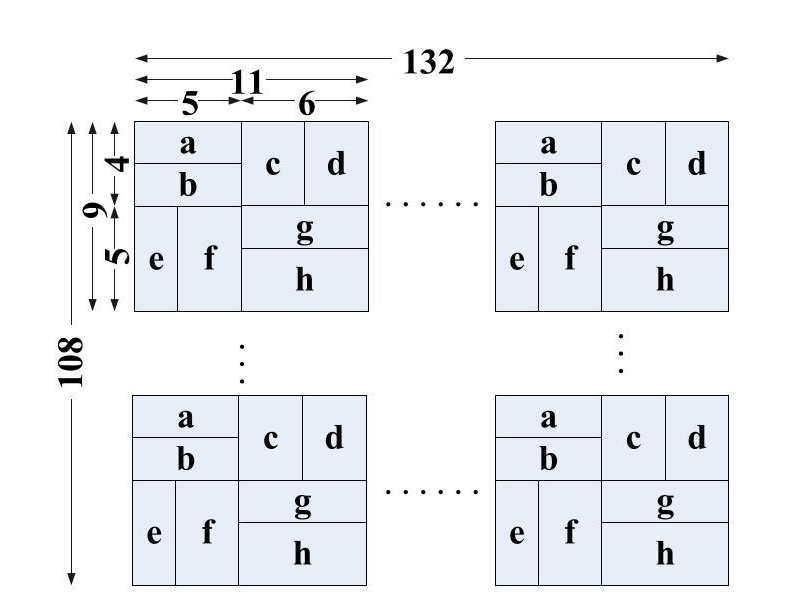
\includegraphics[width=\textwidth]{dados/figuras/sf_division.png}
    \fonte{\citeauthor{mao2015sceneframe}}
    \label{fig:divsceneframe}
\end{figure}


O artigo também propõe uma alternativa para diminuir o espaço de memória utilizado para armazenar as assinaturas, visto que o banco de dados dos vídeos pode ser grande. Para isso, é proposta uma técnica chamada quantificação quaternária, na qual os valores são classificados de acordo com um \textit{threshold}, calculado dinamicamente para cada quadro.

O primeiro limiar, utilizado para as $144$ médias de intensidade, é obtido da seguinte maneira, onde $m_i$ representa cada valor dentro do conjunto $M$ de médias de intensidade:

\begin{enumerate}
\item Para todo $m_i$ em $M$, é calculado o valor absoluto $a_i = abs(m_i - 128)$, obtendo novos valores $A$.
\item Os valores de $A$ são ordenados crescentemente.
\item O limiar $ThM$ utilizado será $a_i$ onde $i = floor(0.25*144)$.
\end{enumerate}

Cada valor $m_i$ é então definido através da Equação \ref{eq:mediaquart}, podendo variar de $[0 - 3]$ .

\begin{equation}
	\label{eq:mediaquart}
	m_i = 
     \begin{cases}
       \text{3,} &\quad\text{Se } m_i-128 > \text{ThM} \\
       \text{2,} &\quad\text{Se } 0 < m_i - 128 \le \text{ThM} \\
       \text{1,} &\quad\text{Se } -\text{ThM} < m_i - 128 \le 0 \\
       \text{0,} &\quad\text{Se } m_i - 128 \le -\text{ThM} \\ 
     \end{cases}
\end{equation}

 \begin{figure}[h]
      \centering
      \caption{Diagrama do algoritmo baseado em quadros de cena.}
      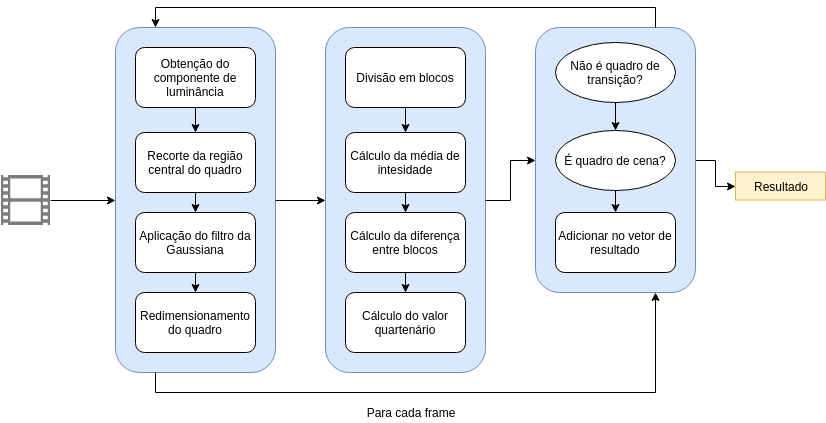
\includegraphics[width=0.96\textwidth]{dados/figuras/SceneFrame.png}
      \fonte{Autoria própria}
       	\label{fig:dia_sceneframe}
    \end{figure}  

% --------------------------------------------------------------------------------------------------
%
% RBP
\subsection{Assinatura baseada em padrões binários por região}
% --------------------------------------------------------------------------------------------------


O descritor apresentado por \citeauthor{kim2014rotation} propõe criar uma assinatura que seja robusta e singular para ataques dos tipos \textit{rotação} e \textit{espelhamento}. Trata-se de um descritor local que utiliza a dimensão espacial dos quadros do vídeo para a extração da assinatura. 

O método divide o quadro em regiões na forma de círculos, então divide os círculos em sub-regiões, ou seja, sub-círculos. Dessas sub-regiões, o algoritmo gera dois padrões binários com a justificativa de preservar as informações da dimensão espacial do quadro e dessa forma manter a robustez da assinatura em relação aos ataques de rotação e espelhamento. O  primeiro padrão binário  \textit{(RBP, Region Binary Pattern)} representa uma única região circular, enquanto o segundo padrão binário representa a relação entre a primeira região e as regiões adjacentes. Após, esses dois padrões são agrupados e concatenados em um vetor, que é a assinatura resultante do algoritmo.

 \begin{figure}[h]
      \centering
      \caption{Diagrama do algoritmo baseado padrões binários por região}
      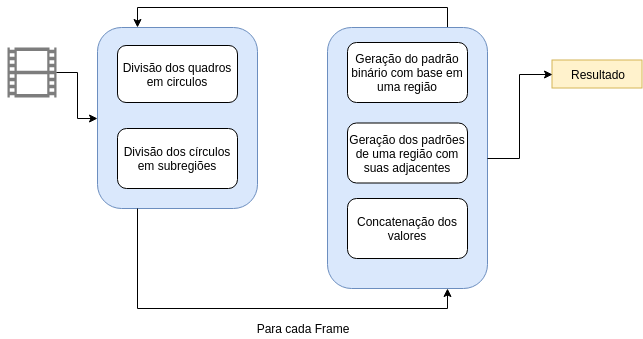
\includegraphics[width=0.96\textwidth]{dados/figuras/RBP.png}
      \fonte{Autoria própria}
       	\label{fig:dia_rbp}
    \end{figure}  

    
% --------------------------------------------------------------------------------------------------
%
% WAVELETS
%
% --------------------------------------------------------------------------------------------------

\subsection{Assinatura baseada em wavelets}
\label{wavelets}

Esta abordagem foi escolhida por ter sido projetada especialmente para ser robusta a uma variedade de ataques fotométricos, como modificações em contraste, brilho, contaminação por ruído e desfoque, inserção de logos, bordas e mudança de formato do quadro. Para se tornar ainda mais robustas a esses ataques, \citeauthor{Dutta2013} também realiza uma etapa de pré-processamento em que possíveis bordas dos quadros são removidas, então o ruído das imagens é removido através de um filtro gaussiano e finalmente o histograma de cada quadro é equalizado. 

Após a etapa de pré-processamento, para serem utilizados como entrada para este algoritmo, os vídeos devem ser transformados para escala de cinza e ter suas intensidades normalizadas para o intervalo $[0,1]$. A assinatura proposta por \citeauthor{Dutta2013} é composta de uma parte baseada na transformada de Haar e em outra parte baseada na distribuição espacial de gradientes.

 Para gerar a assinatura é necessária uma imagem $I$, obtida após a conversão para escala de cinza e normalização. São aplicadas $n$ iterações da transformada de Haar para computar e gerar as bandas $HH, LH, HL$ e $LL$. 
 
 Fórmula para computar energia de $LH$, $HL$, $HH$: $\frac{1}{MN}\sum_{x=1}^M \sum_{y=1}^N |\mathbb{I}(x,y)|$;
 
 %Para i de 1 até $n$, onde $n$ é o número de iterações da transformada de Haar:
%   \begin{enumerate}
%     \item Aplicar a transformada de Haar sobre $I$ para obter um vetor com ($LL, LH, HL, HH$);
%     \item Computar energia de $LH$, $HL$, $HH$ \footnote{$  \frac{1}{MN}\sum_{x=1}^M \sum_{y=1}^N |\mathbb{I}(x,y)|$};
%   \end{enumerate}
 Em seguida, computa-se a energia da subimagem $I$ somente do último valor de $LL$ e então esses valores são concatenados em um vetor. Finalmente, os valores de energia obtidos nos passos anteriores são concatenados resultando na assinatura do vídeo.

% \begin{figure}[h]
%   \centering
%   \begin{tabular}{ccc}
%     \centering
%     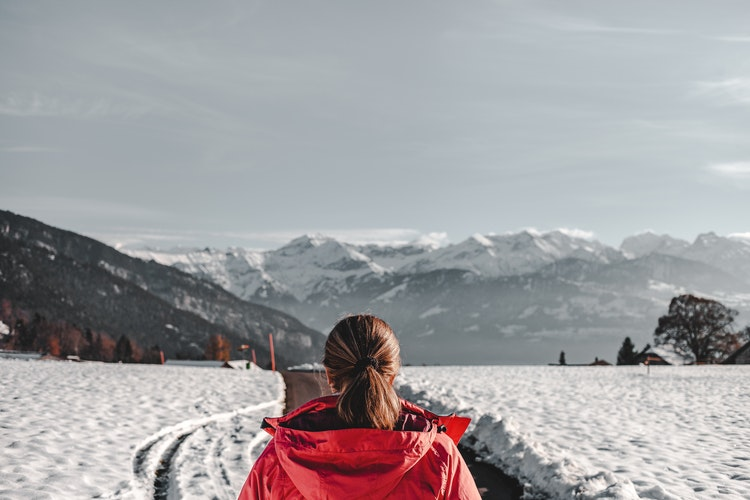
\includegraphics[width=0.45\textwidth]{dados/figuras/original} & 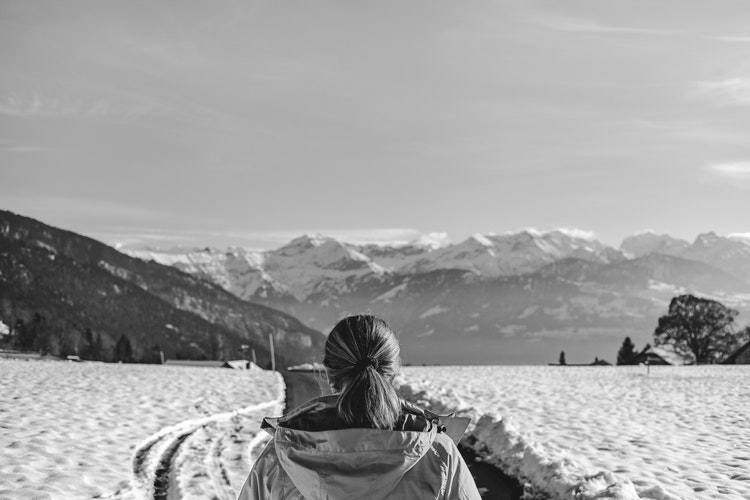
\includegraphics[width=0.45\textwidth]{dados/figuras/original_bw} \\ 
%      a. Quadro original & b. Quadro em escala de cinza \\
%     \multicolumn{2}{c}{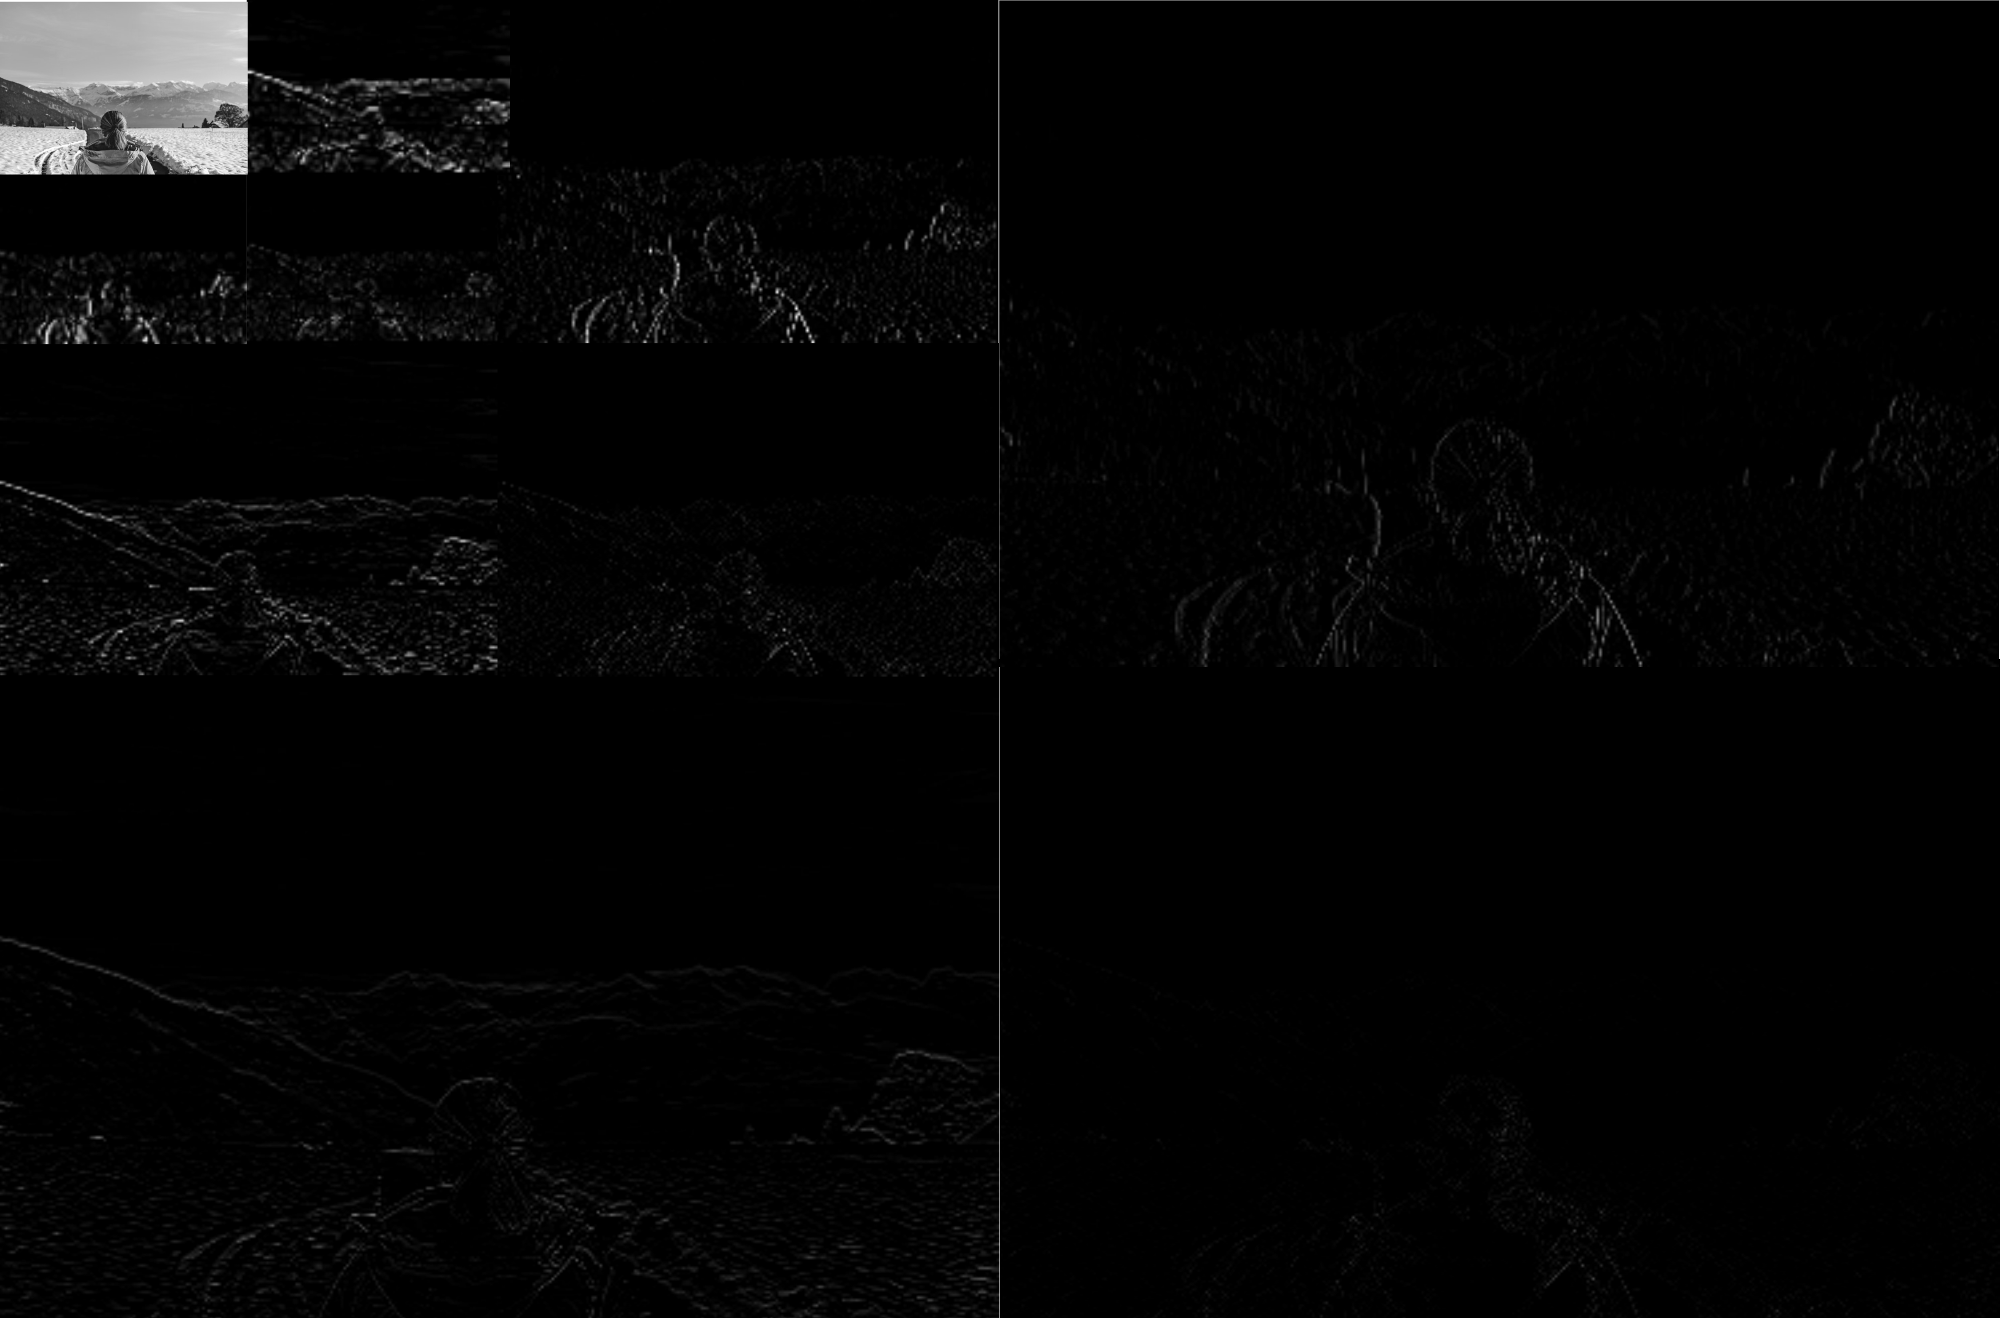
\includegraphics[width=0.94\textwidth]{dados/figuras/wavelet_result_menor}} \\
%     \multicolumn{2}{c}{c. Após transformada de Haar}
%   \end{tabular}
%   \caption{Sequência de transformações feitas pelo algoritmo}
% %   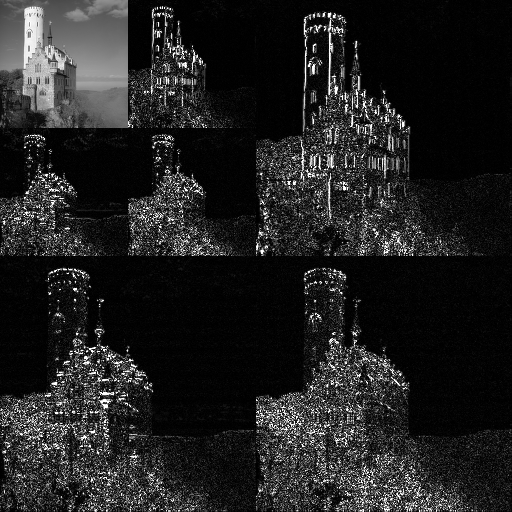
\includegraphics[width=0.8\textwidth]{dados/figuras/haar.png}
% %   \caption{Resultado da Transformada de Haar. Os cantos superior direito, inferior esquerdo e inferior direito são, respectivamente, a derivada na horizontal(LH),derivada na vertical(HL) e derivada na diagonal(HH). O canto superior esquerdo é subdividido $N$ vezes em LH,HL e HH até o último nível em que não há mais divisão e que se chama LL}
%   \label{figure:haar}
% \end{figure}



% A assinatura é gerada a partir de um quadro $I$ já pré-processado, em que é aplicada a transformada de Haar com um nível e obter um vetor com $LL,LH,HL,HH$. Então, computa-se o gradiente de $LL$ \footnote{A imagem LL é usada pois contém menos ruído que a imagem original graças à transformada de Haar} e a imagem de gradiente é dividida em $N_p$ partições com o mesmo tamanho. O penúltimo passo é, para cada partição, computar um histograma de gradiente. Finalmente, os histogramas são concatenados para obter o a assinatura.


 \begin{figure}[h]
      \centering
      \caption{Diagrama do algoritmo baseado em wavelets}
      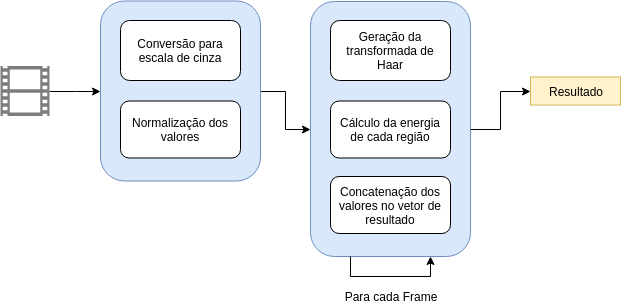
\includegraphics[width=0.96\textwidth]{dados/figuras/Wavelet.png}
      \fonte{Autoria própria}
       	\label{fig:dia_wavelet}
    \end{figure}  



         % Revisão de Literatura
% % \chapter{Desenvolvimento}
\label{sec:desenv}
Estudaremos em detalhes os algoritmos das seguintes seções.


% --------------------------------------------------------------------------------------------------
%
% MEDIDA ORDINAL
%
% --------------------------------------------------------------------------------------------------
\section{Assinatura de vídeo baseada na medida ordinal}
\label{sec:med_ordinal}

	O algoritmo proposto por \cite{hua2004robust} baseia-se na intensidade dos \textit{pixels} de cada quadro para compor a assinatura. O que se propõe é que, primeiramente, a taxa de amostragem, ou seja, a taxa de quadros por segundo (FPS, do inglês \textit{frames per second}) do vídeo de entrada seja padronizada, para que a assinatura gerada fique mais compacta e seja tolerante a diferentes formatos de compressão, por exemplo. Além disso, o vídeo é convertido para escala de cinza.

Após esse pré-processamento, para cada quadro é realizada a divisão em $M \times N$ blocos, como pode ser observado na Figura \ref{fig:medidaord}, bem como o cálculo da intensidade média para cada um dos blocos. Esses valores são então colocados em ordem crescente e representam cada elemento que compõe a assinatura.

	\begin{figure}[h]
        \centering
        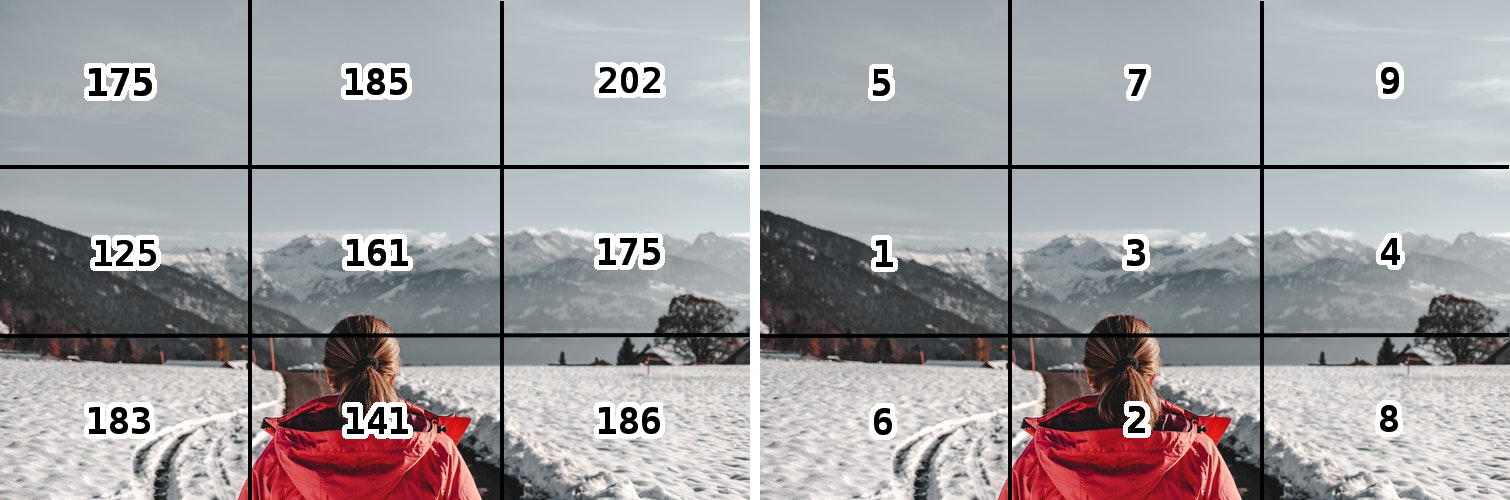
\includegraphics[width=0.8\textwidth]{dados/figuras/mo_final.png}
        \caption{Exemplo com a divisão em blocos, cálculo das intensidades médias e ordem atribuída a cada valor. Referência: \cite{sylvio2015}}
    	\label{fig:medidaord}
    \end{figure}


% --------------------------------------------------------------------------------------------------
%
% GRADIENTE
%
% --------------------------------------------------------------------------------------------------


\section{Assinatura de vídeo baseada em gradientes}
\label{sec:gradientes}

	Este algoritmo, proposto por \cite{lee2008robust}, utiliza a distribuição dos gradientes para geração de assinaturas. O primeiro passo é definir uma taxa de quadros por segundo (fps) fixa, além da conversão para escala de cinza. Outro procedimento utilizado é o redimensionamento dos quadros, tornando o  método robusto independente da mudança de resolução do vídeo. Em seguida, o gradiente dos \textit{pixels} de cada quadro é calculado da seguinte forma. Encontram-se os gradientes $\mathbb{G}x$ e $\mathbb{G}y$ através da equação \ref{eq:gmatrix}.

\begin{equation}
  \label{eq:gmatrix}
  \begin{bmatrix}
    \mathbb{G}x
    \\ 
    \mathbb{G}y
  \end{bmatrix}= 
  \begin{bmatrix}
    \partial I/\partial x
    \\ 
    \partial I/\partial y
  \end{bmatrix}=
  \begin{bmatrix}
    \mathbb{I}(x+1, y) - \mathbb{I}(x-1,y)
    \\ 
    \mathbb{I}(x, y+1) - \mathbb{I}(x,y-1)
  \end{bmatrix}
\end{equation}
    
	O quadro é então dividido em $M\times N$ blocos, para quais é determinado o valor do centroide dos gradientes, criando assim um vetor com $(M \times N)$ elementos. Para isso, é necessário encontrar a magnitude \textit{$w(x,y)$} e a orientação \textit{$\Theta(x,y)$}, conforme mostra a Equação \ref{eq:mag-or}.
    
\begin{equation}
	\label{eq:mag-or}
    w(x,y) = \sqrt{\mathbb{G}x^{2} + \mathbb{G}y^{2}}
\qquad
\Theta(x,y) = tan^{-1}\left (\frac{\mathbb{G}y}{\mathbb{G}x} \right)
\end{equation}
    
    Em seguida o centroide para cada bloco é obtido a partir do somatório do produto da magnitude e orientação, dividido pela somatória de todas as magnitudes daquele bloco, como pode ser observado na Equação \ref{eq:gradientes}:
    
\begin{equation}
	\label{eq:gradientes}
	[i] = \frac{\sum_{x,y \in b[i]} w(x,y)\Theta (x,y)}{\sum_{x,y \in b[i]} w(x,y)}
\end{equation}
    
% --------------------------------------------------------------------------------------------------
%
% FRAME DIFF
%
% --------------------------------------------------------------------------------------------------

\section{Assinatura de vídeo baseada na diferença entre quadros}
\label{sec:framediff}

  O algoritmo proposto por \cite{cook2011efficient} utiliza características globais, como luminância e diferença de luminância intra-quadros, para uma assinatura robusta (ao utilizar medidas que refletem a estrutura temporal do conteúdo) e eficiente (ao utilizar medidas simples de serem calculadas e comparadas). Para cada quadro de um vídeo são coletadas as seguintes características: 

  \begin{itemize}
    \item \textit{timestamp}, o tempo do quadro relativo ao início do vídeo
    \item Luminância Total ($Y$), soma da luminância de todos os pixels de um frame
    \item Luminância Máxima ($Y_{max}$), o valor do pixel mais brilhante do quadro
    \item Área do Frame ($A$), largura $\times$ altura do vídeo, útil para normalização
    \item Luminância diferencial ($dY$), a diferença absoluta de luminância pixel a pixel do quadro atual como quadro que estava visível há 100 milisegundos, a diferença resultante é somada (como mostra a equação \ref{eq:framediff}). 
  \end{itemize}

\begin{equation}
	\label{eq:framediff}
	dY = \sum_{x,y \in  \mathbb{I,J}} |\mathbb{I}(x,y) - \mathbb{J}(x,y)|
\end{equation} 

  Após a obtenção das características primárias, estas passam por um processo de refinamento no qual os vetores $Y$ e $dY$ são passados por filtros passa-baixa (figura ~\ref{fig:framediff-passa-baixa}). Além disso, duas outras características são derivadas das características principais e visam medir o quão imóvel uma sequência de frames é. Para isso, são definidas as medidas "Quietude" (equação \ref{eq:framediff-credits}) e "Créditos" (equação \ref{eq:framediff-stillness}).

  \begin{equation}
    \label{eq:framediff-stillness}
    Quietude = 100 \times \left(\sqrt{\frac{\ln\frac{dY}{A}}{\ln256}}\right) \\
  \end{equation}

  \begin{equation}
    \label{eq:framediff-credits}
    Creditos = 100 \times \frac{\frac{Y_{max}}{256} + \left( 1 - \left( \frac{\ln\frac{Y}{A}}{\ln256} \right)^2\right)}{2}
  \end{equation}


\begin{figure}[h]
  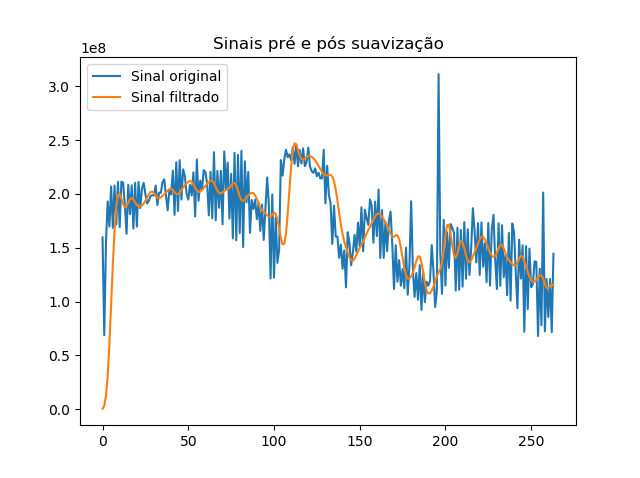
\includegraphics[width=0.7\textwidth]{dados/figuras/filtro_passa_baixa}
  \caption{Linha azul mostra os valores originais do vetor $dY$ e a linha alaranjada mostra os valores pós filtro passa-baixa}
  \label{fig:framediff-passa-baixa}
\end{figure}


A figura \ref{fig:framediff-comparacao} mostra a característica $dY$ plotada para um vídeo original e sua versão distorcida com efeitos de desfoque (\textit{blur}) e adição de legenda, além de mostrar os valores de $dY$ para outro vídeo não relacionado.

\begin{figure}[h]
  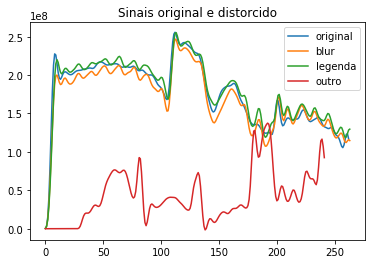
\includegraphics[width=0.7\textwidth]{dados/figuras/dy}
  \caption{Comparação entre os vetores de característica $dY$ gerados para um vídeo, uma cópia com o efeito de desfoque, uma cópia com uma legenda inserida, e um outro vídeo qualquer}
  \label{fig:framediff-comparacao}
\end{figure}


Para realizar a comparação entre duas assinaturas, \citeauthor{cook2011efficient} propõe o uso da distância de Manhattan normalizada, como descrito na fórmula \ref{eq:dist-manhattan}. Além disso, é proposto o uso de uma combinação das características $Y$ e $dY$ na comparação, pois separadas elas obteram $0.579\%$ e $0.157\%$ de falsos positivos, respectivamente, enquanto que a combinação das duas características obteve apenas $0.018\%$. 

\begin{equation}
  Distancia(a,b) = \frac{\sum_i|a_i - b_i|}{|a|}
  \label{eq:dist-manhattan}
\end{equation}

%% --------------
%% TODO: explicar comparação
%% --------------

%   Dados dois quadros $\mathbb{I}$ e $\mathbb{J}$, a assinatura temporal desenvolvida por \cite{cook2011efficient} utiliza dois componentes principais para sua construção. O primeiro é a luminância total $Y$, ou seja, a soma dos \textit{pixels} do \textit{frame}, representando o brilho total da imagem. O outro parâmetro é $dY$, ou diferencial de luminância, sendo a diferença do quadro atual com o quadro anterior. $dY$ é uma métrica para saber o quanto a luminância varia com a mudança dos quadros no vídeo.  Essa variação pode acontecer, segundo o autor, a partir do movimento da câmera, corte entre cenas e objetos e pessoas que entram ou saem de cena. 
    
%    O  valor de $dY$ pode ser obtido através da Equação \ref{eq:framediff} \cite{sylvio2015}: 

% Portanto cada \textit{frame} será representando por uma tupla $(Y, dY)$.
    
% --------------------------------------------------------------------------------------------------
%
% WAVELETS
%
% --------------------------------------------------------------------------------------------------

\section{Assinatura de vídeo baseada em wavelets}

Esta abordagem foi escolhida por ter sido projetada especialmente para ser robusta a uma variedade de ataques fotométricos e de pós-produção, como modificações em contraste, brilho, contaminação por ruído e desfoque, inserção de logos, bordas e mudança de formato do quadro. Para se tornar ainda mais robustas a estes ataques, \citeauthor{Dutta2013} também descreve um fluxo de pré-processamento. % abordado na Seção \ref{sec:preprocessamento}.

Após a etapa de pré-processamento e para ser usado como entrada para este algoritmo, os vídeos devem ser transformados para escala de cinza e ter suas intensidades normalizadas para o intervalo $[0,1]$. A assinatura proposta por \citeauthor{Dutta2013} é composta de uma parte baseada na transformada de Haar e em  outra baseda na distribuição espacial de gradientes.

\subsection{Transformada de Haar}

A transformada de Haar consiste em separar um sinal (ou quadro, neste caso) em 4 partes: 

\begin{itemize}
\item $LL$, que contém $1/4$ dos dados originais, removendo os detalhes.
\item $LH$, que contém a derivada na horizontal do quadro
\item $HL$, que contém a derivada na vertical do quadro
\item $HH$, que contém a derivada na diagonal do quadro
\end{itemize}

Ela pode ser aplicada de forma recursiva $n$ vezes, usando o quadro $I$ como entrada inicial do algoritmo e o $LL$ como entrada das chamadas subsequentes. Um exemplo do resultado da transformada de Haar pode ser visto na Figura \ref{figure:haar}.

\subsection{Assinatura baseada em wavelets}

\begin{enumerate}
\item Seja $I$ a imagem obtida após conversão para escala de cinza e normalização
% \item $F_i$ <- $F$
\item Para i de 1 até $n$, onde $n$ é o número de iterações da transformada de Haar
  \begin{enumerate}
    \item Aplicar a transformada de Haar sobre $I$ para obter um vetor com ($LL, LH, HL, HH$)
    \item Computar energia de $LH$, $HL$, $HH$ \footnote{$  \frac{1}{MN}\sum_{x=1}^M \sum_{y=1}^N |\mathbb{I}(x,y)|$}
  \end{enumerate}
\item Computar a energia da subimagem $I$, do último valor de $LL$ e concatenar estes valores em um vetor,
\item Concatenar os valores de energia obtidos nos passos anteriores para obter o descritor
\end{enumerate}

\begin{figure}[h]
  \centering
  \begin{tabular}{ccc}
    \centering
    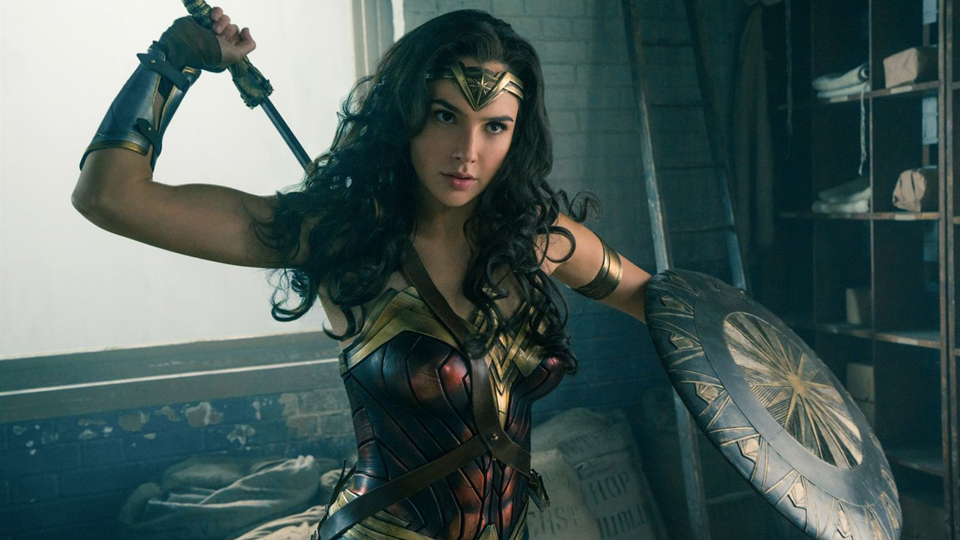
\includegraphics[width=0.45\textwidth]{dados/figuras/ww.jpg} & 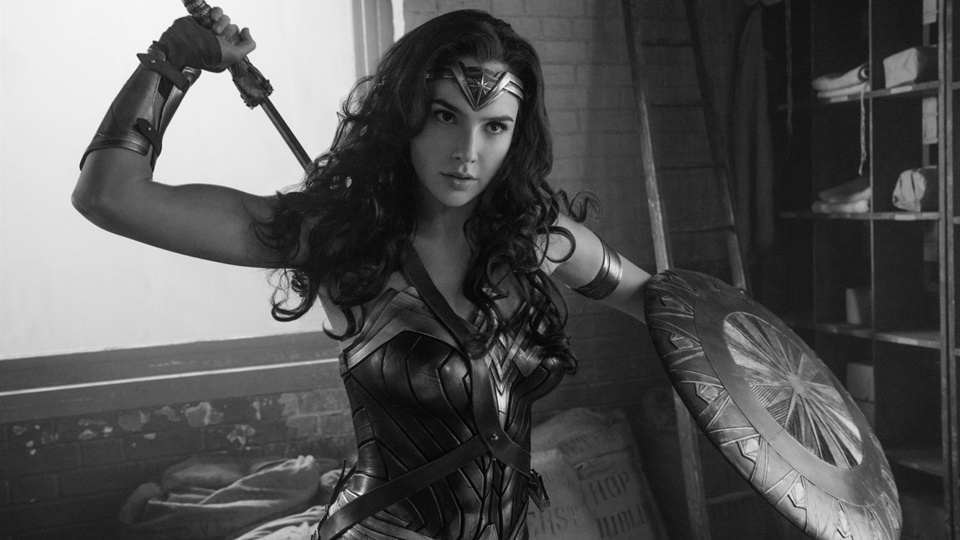
\includegraphics[width=0.45\textwidth]{dados/figuras/ww_bw.jpg} \\ 
     a. Quadro original & b. Quadro em escala de cinza \\
    \multicolumn{2}{c}{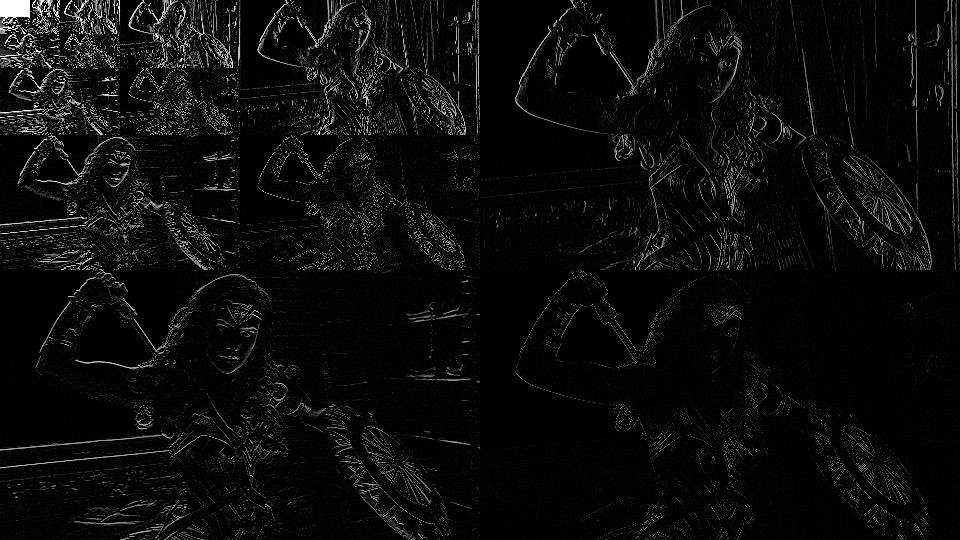
\includegraphics[width=0.94\textwidth]{dados/figuras/ww_haar_.jpg}} \\
    \multicolumn{2}{c}{c. Após transformada de Haar}
  \end{tabular}
  \caption{Sequência de transformações feitas pelo algoritmo utilizando um quadro do filme Mulher Maravilha}
%   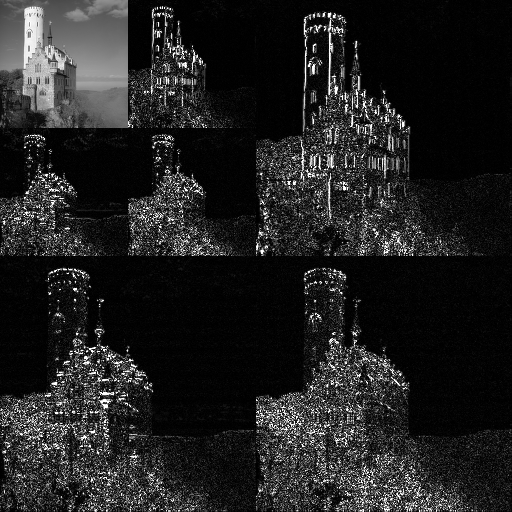
\includegraphics[width=0.8\textwidth]{dados/figuras/haar.png}
%   \caption{Resultado da Transformada de Haar. Os cantos superior direito, inferior esquerdo e inferior direito são, respectivamente, a derivada na horizontal(LH),derivada na vertical(HL) e derivada na diagonal(HH). O canto superior esquerdo é subdividido $N$ vezes em LH,HL e HH até o último nível em que não há mais divisão e que se chama LL}
  \label{figure:haar}
\end{figure}

\subsection{Assinatura baseada em distribuição espacial de gradientes}

\begin{enumerate}
\item Dado um quadro $I$ já pré-processado, aplicar a transformada de Haar com um nível e obter um vetor com $LL,LH,HL,HH$
\item Computar o gradiente de $LL$\footnote{A imagem LL é usada pois contém menos ruído que a imagem original graças à transformada de Haar}
\item Dividir a imagem de gradiente em $N_p$ partições com o mesmo tamanho
\item Para cada partição, computar um histograma de gradiente
\item Concatenar os histogramas  para obter o descritor
\end{enumerate}

% --------------------------------------------------------------------------------------------------
%
% SCENE FRAME
%
% --------------------------------------------------------------------------------------------------

\section{Assinatura baseada em quadros de cena}

  Outra abordagem, proposta por \citeauthor{mao2015sceneframe}, é baseada na assinatura de quadros de cena. De acordo com os autores, os quadros de cena podem ser \textit{intraframes}, ou seja, quadros que iniciam tomadas, quanto \textit{interframes}, contanto que sigam as características descritas em \ref{sec:quadrocena}.
    
    O algoritmo fundamenta-se na ideia de que as chances de existirem cinco quadros de cena seguidos é extremamente baixa, por isso são selecionados apenas os cinco primeiros quadros de cena de um vídeo. A forma como estes são determinados é descrita na Seção \ref{subsec:fptsceneframe}.

\subsection{A extração de assinatura}
\label{subsec:fptsceneframe}

% \begin{algorithm}
	\caption{HUGO \cite{hugo}}
	\label{alg:hugo}
	\KwIn{Todos os PIXELS da imagem de cobertura X}
	\KwOut{A estego imagem Y}

	\For { $(i, j)$ in $PIXELS$ } {

        \tcp{Calcula o impacto da codificação de +1}

		\algstat{stego\_plus \gets X.copy()}

		\algstat{stego\_plus[i][j]++}

		\algstat{embed\_impact\_plus[i][j] \gets D(X, stego\_plus)}

        \tcp{Calcula o impacto da codificação de -1}

		\algstat{stego\_minus \gets X.copy()}

		\algstat{stego\_minus[i][j]--}

		\algstat{embed\_impact\_minus[i][j] \gets D(X, stego\_minus)}
	}

	\tcp{Mínimo, elemento a elemento}

	\algstat{embed\_impact\_min \gets min(embed\_impact\_plus, embed\_impact\_minus)}

	\tcp{\textit{Syndrome Trellis-Code}}

	$\mathrm{pixels\_to\_change} \gets \mathrm{minimize\_embed\_impact}(LSB(X), \mathrm{embed\_impact\_min, message})$

	\algstat{Y \gets X}

	\eIf{ \algstat{model\_correction\_step\_enabled} } {
		\For { $(i, j)$ in $pixels\_to\_change$ } {
			\algstat{correction\_plus \gets Y}

			\algstat{correction\_plus[i][j]++}

			\algstat{dp \gets D(X, correction\_plus)}

			\algstat{correction\_minus \gets Y}

			\algstat{correction\_minus[i][j]--}

			\algstat{dm \gets D(X, correction\_minus)}

			\eIf{ $dp < dm$ }{
				$Y[i][j]++$
			}{
				$Y[i][j]--$
			}
		}
	}{
		\For { $(i, j)$ in $pixels\_to\_change$ } {
			\eIf{ $embed\_impact\_plus[i][j] < embed\_impact\_minus[i][j]$ }{
				$Y[i][j]++$
			}{
				$Y[i][j]--$
			}
		}
	}
	
\end{algorithm}


A obtenção da assinatura, para \citeauthor{mao2015sceneframe}, é realizada para todos os quadros, para então serem comparadas e selecionadas. Como pode ser observado no Diagrama \ref{dig:sceneframe}, os quadros passam por um pre-processamento, onde o componente de luminância é obtido. O quadro então é recortando, mantendo-se apenas sua região central e, por fim, redimensionado para o tamanho definido de $3/4$QCIF, ou seja, $(108\times132)$.

% Após o processamento inicial, o quadro é então dividido em $144$ pedaços menores, de tamanho $(9\times11)$, cuja média de intensidade irá compor parte da assinatura deste quadro. Além dos $144$ valores, o descritor é composto também por $576$ elementos diferenciais, totalizando $720$ valores. Para obter esses elementos, cada fragmento é dividido em oito elementos menores, como mostra a Figura \ref{fig:divsceneframe}, e então é realizada a subtração de $a - b$, $c - d$, $e - f$ e $g - h$.

\begin{figure}[h]
  \centering
    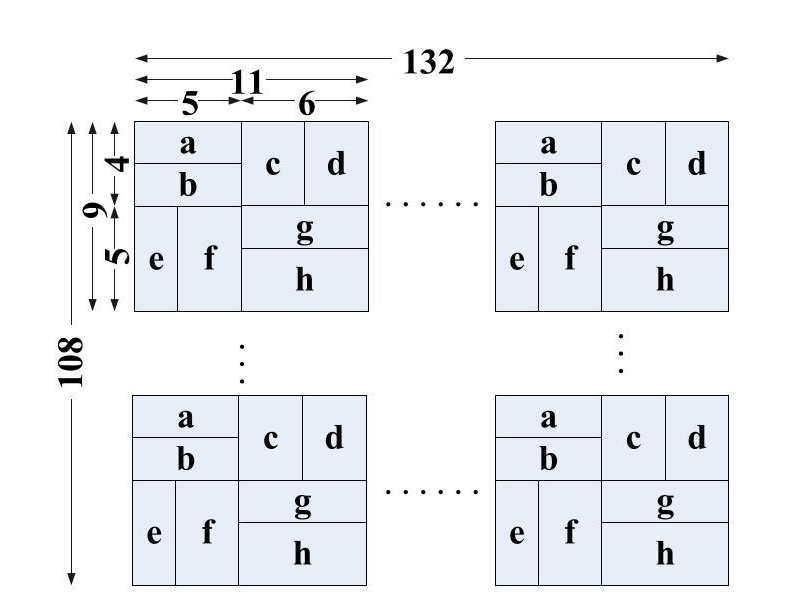
\includegraphics[width=\textwidth]{dados/figuras/sf_division.png}
    \caption{Divisão da imagem para cálculo dos elementos diferenciais. Referência: \citeauthor{mao2015sceneframe}}
    \label{fig:divsceneframe}
\end{figure}

\subsection{Diminuição do espaço de memória utilizado}

O artigo também propõe uma alternativa para diminuir o espaço de memória utilizado para armazenar as assinaturas, visto que o banco de dados dos vídeos pode ser grande. Para isso, é proposta uma técnica chamada qualificação quaternária, na qual os valores são classificados de acordo com um \textit{threshold}.


% --------------------------------------------------------------------------------------------------
%
% RBP
%
% -------------------------------------------------------------------------------------------------- %include realizado na revisao da literatura
% METODOLOGIA------------------------------------------------------------------

\chapter{Metodologia}
\label{chap:metodologia}

A metodologia do projeto consiste das seguintes etapas:

\begin{enumerate}
\item Revisão da literatura;
\item Definição e obtenção da base de vídeos
\item Definição dos algoritmos;
\item Implementação dos algoritmos; 
\item Definição do método de comparação;
\item Implementação do método de comparação;
\item Validação das implementações;
\item Definição dos experimentos;
\item Experimentos;
	\begin{enumerate}
		\item Compilação de uma nova base de vídeos;
        \item Geração dos vídeos com distorções;
        \item Geração da assinatura para todos os vídeos;
        \item Aplicação do método de comparação;
			% Especificações dos vídeos que serão utilizados
			% Dimensão, duração, taxa de frames, conteúdo dos videos, extensão (compressão), vídeos problemáticos
	\end{enumerate}
\item Análise dos resultados;
% \item Conclusão
\end{enumerate}

\section{Revisão da Literatura}

Foi realizada uma revisão da literatura pertinente à pesquisa. Este método de revisão da literatura foi escolhido pois define formas de identificar, interpretar e avaliar pesquisas disponíveis coerentes com o tema. 

Além de artigos recentes relacionados à área, as referências de \citeauthorsylvio2015} também foram utilizadas na revisão e passaram pelo processo de filtragem, uma vez que este trabalho baseia-se no de \citeauthorsylvio2015}.

\subsection{Definições}

O primeiro passo da revisão é a definição das perguntas que devem ser respondidas, das palavras-chave a serem utilizadas e dos critérios de exclusão de artigos. O intuito da revisão é definido a seguir:

\begin{itemize}
\item encontrar algoritmos para tratar diferentes problemas relacionados à descrição de vídeos e compreender seu funcionamento;
\item encontrar métodos de \textit{matching} de descritores;
\item encontrar e compilar uma base de vídeos para realização dos testes;
\end{itemize}

Além das referências de \citeauthorsylvio2015}, foram escolhidos repositórios em português e em inglês para a busca das palavras-chave. Os repositórios estão definidos na tabela~\ref{tabela:listarepositorios} enquanto as palavras-chave na tabela \ref{tabela:palavraschave}.

\begin{table}[h]
\resizebox{\textwidth}{!}{
\begin{tabular}{|l|l|l|}
	\hline
    Língua & Repositórios & Endereço \\
    \hline
    \multirow{4}{*}{Inglês} & IEEE & \url{http://ieeexplore.ieee.org/Xplore/home.jsp} \\
    & ScienceDirect & \url{http://www.sciencedirect.com/} \\
    & ACM & \url{http://dl.acm.org/} \\
    & Google Scholar & \url{https://scholar.google.com.br/} \\
    \hline
    \multirow{2}{*}{Português} & Periódico CAPES & \url{http://www-periodicos-capes-gov-br.ez48.periodicos.capes.gov.br} \\
    & SciELO & \url{http://www.scielo.org} \\
    \hline
\end{tabular}
}
\caption[Lista de repositórios utilizados]{Lista de repositórios utilizados.}
\label{tabela:listarepositorios}
\end{table}

\begin{table}[h]
\resizebox{\textwidth}{!}{
\begin{tabular}{|l|l|}
\hline
Português & Inglês \\
\hline
Detecção de cópia baseada em conteúdo & Content-Based Video Copy Detection\\
\hline
Descritor de vídeo & Video fingerprint \\
\hline
Detecção de cópia de video & video copy detection \\
\hline
\end{tabular}
}
\caption{Palavras-chave utilizadas na revisão sistemática.}
\label{tabela:palavraschave}
\end{table}


Para auxiliar na indexação dos artigos achados e na sua utilização como base para este trabalho, os artigos foram divididos em categorias, como mostra a tabela \ref{tabela:categoriaartigos}.

\begin{table}[h]
\resizebox{\textwidth}{!}{
	\begin{tabular}{|l|l|l|}
    \hline
	& Categoria & Descrição \\
    \hline
    1 & Descritores Globais & Algoritmos que produzem descritores baseados em características globais de um vídeo \\
    \hline
    2 & Descritores Locais & Algoritmos que produzem descritores baseados em características locais de um vídeo \\
    \hline
    3 & Comparação de Descritores & Métodos para comparação de descritores \\
    \hline
	\end{tabular}
}
    \caption{Categorização dos artigos.}
    \label{tabela:categoriaartigos}
\end{table}

\section{Definição e Obtenção da Base de Vídeos}

Foi escolhida a base UCF50 - Action Recognition Data Set \citeauthorreddy2013recognizing} e embora seja utilizada para reconhecimento de movimento humano baseado em ações, como por exemplo ciclismo, natação, caminhada com o cachorro, TaiChi, etc., os motivos para sua escolha foram a quantidade de vídeos e sua licença de livre utilização. 

Do total de 6.681 itens, foram selecionados 1.264, pois os vídeos estavam fragmentados em diversas cenas, ou seja, apenas uma cena de cada vídeo foi utilizada. Cada cena tem uma duração média de 3 a 9 segundos.

Para cada vídeo selecionado foram aplicadas 14 distorções, totalizando 18.960 itens, sendo destes, 17.696 vídeos resultantes das distorções.

[escrever das 14 distorções]

\section{Definição e implementação dos algoritmos}

Como este trabalho visa continuar a pesquisa em descritores de vídeo baseando-se em \citeauthorsylvio2015}, os primeiros algoritmos estudados e implementados são os três algoritmos já implementados por ele, descritos nas Seções \ref{sec:med_ordinal}, \ref{sec:gradientes} e \ref{sec:framediff}.

Embora \citeauthorsylvio2015} tenha optado por comparar apenas algoritmos de descrição global, devido a sua simplicidade de implementação, neste trabalho serão utilizados tanto descritores locais quanto globais.

POR QUE DOS OUTROS TRÊS ALGORITMOS?
[sao recentes e locais]


Foi escolhida a linguagem Python (versão 2.7.12) para a implementação dos algoritmos por ser multiplataforma e  por sua simplicidade na integração com bibliotecas de alta-performance implementadas em linguagens de baixo nível (C). Isto foi importante pois serão utilizadas as bibliotecas \textit{OpenCV} (versão 3.0.0) e \textit{NumPy} (versão 1.12.1) para manipulação e operação de imagens.

Para a compilação da base de vídeos foi utilizada a biblioteca MagicImage (versão 7.0.7-8-Q16-x64 - Windows), que incluí os programas \textit{convert} e \textit{ffmpeg}, utilizados para conversão de formatos, aplicação de distorções e transformações de vídeo e imagem respectivamente.

\section{Definição e Implementação do método de comparação}




pegar base de assinaturas distrocidas, e para cada distorçao, calcular a distancia para todas as assinaturas originais

pegar as duas menores distancias para cada distorçao de cada vídeo

se a dif do primeiro colocado (primera distancia) for diferente o suficiente para o segundo colocado , entao podemos assumir (podemos?) que encontramos a assinatura do vídeo original

EMBASAR ESSAS PARADAS LOUCAS

\section{Validação das implementações}

Antes de realizar-se qualquer experimento, é necessário que os algoritmos implementados passem por uma etapa de validação que consiste em comparar seus resultados com os dos artigos de base. Para isso serão revisados os artigos dos quais os algoritmos foram retirados, além de códigos disponibilizados através destes trabalhos.

A validação ocorrerá em duas etapas:

\begin{enumerate}
\item teste de software;
\item comparação das saídas dos algoritmos implementados para o trabalho e as implementações originais, dada a mesma entrada.
\end{enumerate}

               % Metodologia
% RESULTADOS-------------------------------------------------------------------

\chapter{Análise e Discussão dos Resultados}
\label{chap:resultados}

Este capítulo discute os resultados obtidos nas duas abordagens de esteganálise estudadas neste trabalho. Como descrito anteriormente, a primeira é baseada no descritor SRM - posteriormente utilizado em um conjunto (\textit{ensemble}) de classificadores - e a segunda em CNNs. 

Conforme detalhado no capítulo anterior, são considerados 12 conjuntos de treinamento, resultantes da aplicação dos algoritmos de esteganografia HUGO, S-UNIWARD e MiPOD para quatro diferentes \textit{payloads}: 0.1, 0.2, 0.4 e 0.6 bpp. Visando facilitar a identificação de um conjunto específico, serão consideradas as siglas definidas na Tabela~\ref{tab:cenariosTrain}, compostas pela primeira letra do nome do algoritmo de esteganografia seguida do valor do \textit{payload} (por exemplo, H6 representa HUGO com \textit{payload} 0.6 bpp).

Além disso, também são definidos 28 conjuntos de teste, listados na Tabela~\ref{tab:cenariosTest}. Cada um deles é identificado por uma sigla composta pela primeira letra do nome do algoritmo de esteganografia utilizado para gerar a estego imagem, seguida por dois valores: um  que representa o STC e outro que identifica o \textit{payload} (por exemplo, H.0.2 representa o HUGO com STC 0 e \textit{payload} 0.2 bpp).

Cada um dos 12 conjuntos de treinamento é utilizado separadamente para treinamento das duas abordagens de esteganálise. Os modelos de classificação resultantes (\textit{ensemble} de classificadores ou CNN) são então aplicados em diferentes conjuntos de teste (x denota a variação para os quatro \textit{payloads}):
\begin{enumerate}%TODO
\item SRM + \textit{Ensemble}: sete conjuntos - H.0.x, H.10.x, S.0.x, S.10.1, S.10.4, S.10.6, M.0.x\footnote{Por limitação de tempo não foram realizados os demais testes.}.
\item CNN: todos os 28 conjuntos listados na Tabela~\ref{tab:cenariosTest} - H.0.x, H.10.x, S.0.x, S.7.x, S.10.x, S.12.x, M.-.x.
\end{enumerate}
Com isso, tem-se um total de 12 $\times$ 7 + 12 $\times$ 28 = 420 resultados.

Na sequência, serão discutidos os resultados obtidos, os quais serão divididos por abordagem de esteganálise e depois por conjunto de treinamento. Ao final, será realizada uma análise geral dos resultados. Os Apêndices \ref{chap:apendiceA} e \ref{chap:apendiceB} mostram tabelas das áreas sob a curva (AUC) obtidas nos testes com SRM e CNN respectivamente.

\clearpage
\section{Resultados com SRM e \textit{Ensemble} de Classificadores}

Em geral, o comportamento da seleção de características é semelhante para todos \textit{payloads}de 1000 à 1400 características. No caso do número de classificadores, os dois \textit{payloads} menores variam de 70 à 80 enquanto os maiores variam de 90 à 100. Tais comportamentos são ilustrado na Figura \ref{fig:srm_train}, para o caso do conjunto de treinamento M1.

\begin{figure}[ht]
\centering
	\subfloat[]{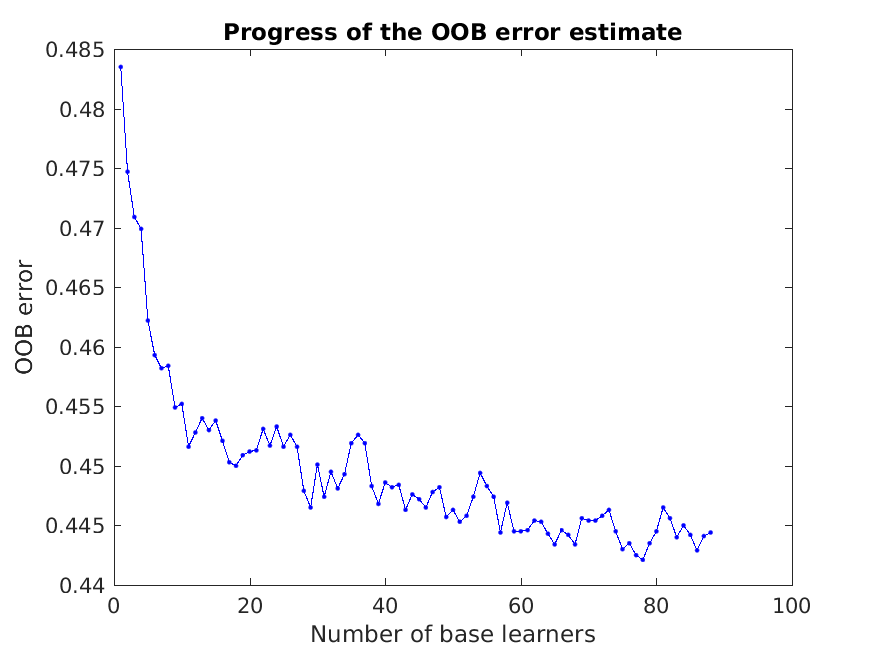
\includegraphics[width=0.7\textwidth]{dados/figuras/oob.png}}\qquad
	\subfloat[]{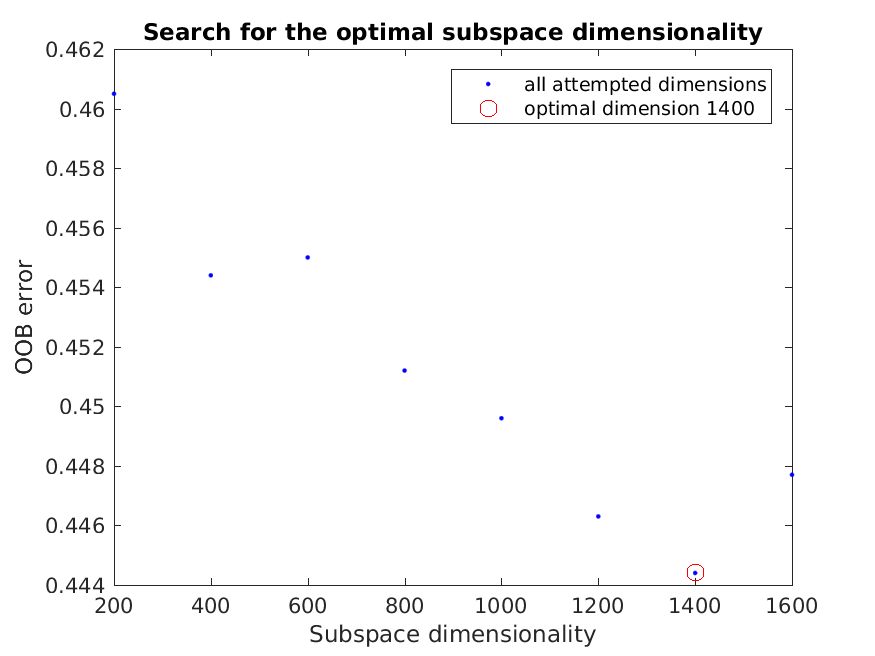
\includegraphics[width=0.7\textwidth]{dados/figuras/dimesion.png}}\\ 

\caption{(a) Variação do OOBe com relação ao número de classificadores para o cojunto de treinamento M1. (b) Variação do OOBe com relação ao número de características para o conjunto de treinamento M1 (Autoria própria).}
\label{fig:srm_train}
\end{figure}

Outro fato interessante é o comportamento dos classificadores base para os diferentes \textit{payloads} de teste. A Figura \ref{fig:votes}(a) mostra a assertividade quando o \textit{payload} de treinamento e teste são próximos, dado que existe uma tendência do indicador estar próximo da extremidade e com os tipos de imagens, estego ou cobertura, na posição desejada.

Além disso, quando o classificador treinado em um conjunto de treinamento com  \textit{payload} alto é aplicado em um conjunto de testes que possui \textit{payload} baixo, o histograma tende a estar mais elevado para a esquerda tanto para as imagens de cobertura quanto para as estego imagens. Isso ocorre porque, como o \textit{payload} de teste é muito menor que o de treino, a rede confunde quase todas as imagens com imagens de cobertura. Esse comportamento é recíproco para \textit{payloads} de treino e teste inversos, porém a confusão ocorre com estego imagens (um exemplo pode ser visto na Figura \ref{fig:votes}(b)).

\begin{figure}[!htb]
\centering
	\subfloat[]{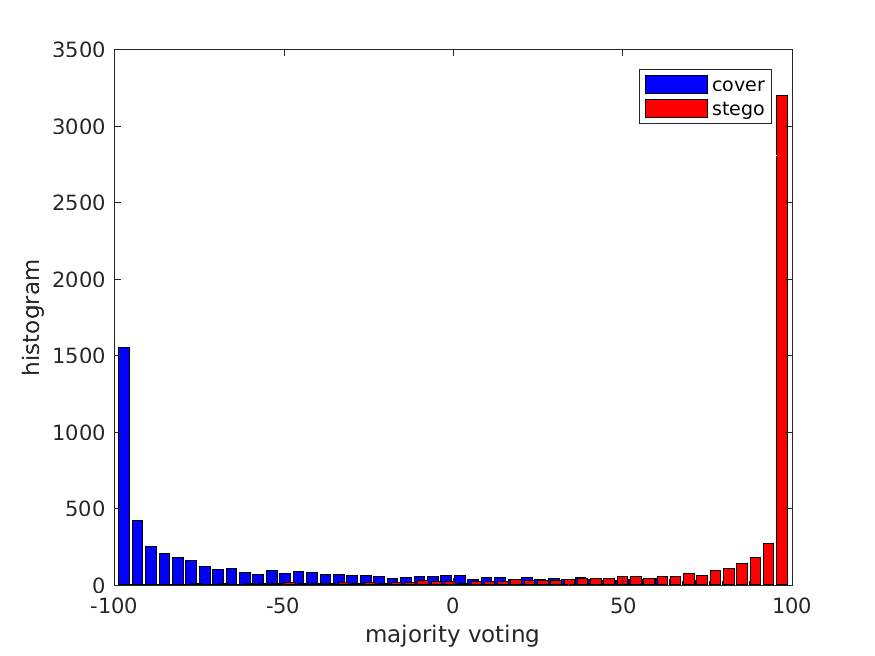
\includegraphics[width=0.45\textwidth]{dados/figuras/voting2.png}}\qquad
	\subfloat[]{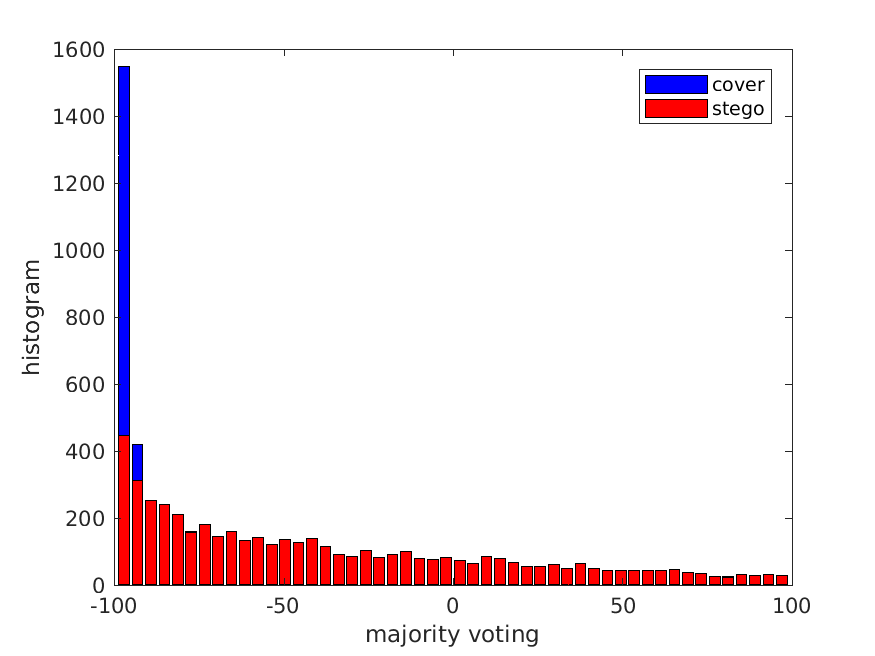
\includegraphics[width=0.45\textwidth]{dados/figuras/voting3.png}}\\ 

\caption{(a) Histograma de votação para o conjunto de treino H4 e de teste H.0.6. (b) Histograma de votação para o conjunto de treino H6 e de teste H.0.1. (Autoria própria)}
\label{fig:votes}
\end{figure}





As seções a seguir apresentarão os resultados da classificação das imagens com o uso do descritor SRM para os 12 diferentes conjuntos de treino.

\clearpage
\subsection{Conjunto de Treinamento H1}

Os resultados para o conjunto de treinamento H1 podem ser vistos na Tabela \ref{tab:srm_h1}. Os melhores resultados foram obtidos com o \textit{payload} de teste igual ao de treino e resultados inferiores nos demais cenários de teste. Essas situações mostram as principais características observadas ao se usar o descritor SRM com \textit{ensemble} de classificadores: melhores performances quando se usando \textit{payload} próximo e mesmo algoritmo de treino e teste, baixa performance ao testar com \textit{payloads} muito distintos do de teste, além da facilidade na detecção do algoritmo HUGO em relação aos outros dois algoritmos.

\begin{table}[!htb]
\centering
\begin{tabular}{c|c|c|c|c|}
\cline{2-5}
\textbf{}                             & \textbf{x = 0.1} & \textbf{x = 0.2} & \textbf{x = 0.4} & \textbf{x = 0.6} \\ \hline
\multicolumn{1}{|c|}{\textbf{H.0.x}}  & 66,23\%          & 72,48\%          & 77,57\%          & 79,31\%          \\ \hline
\multicolumn{1}{|c|}{\textbf{H.10.x}} & \textbf{67,02\%} & \textbf{73,25\%} & \textbf{77,79\%} & \textbf{79,42\%} \\ \hline
\multicolumn{1}{|c|}{\textbf{S.0.x}}  & 58,78\%          & 66,91\%          & 74,68\%          & 78,11\%          \\ \hline
\multicolumn{1}{|c|}{\textbf{S.10.x}} & 59,78\%          & 67,71\%         & 75,20\%          & 78,24\%          \\ \hline
\multicolumn{1}{|c|}{\textbf{M.-.x}}  & 57,86\%          & 64,77\%          & 71,92\%          & 75,61\%          \\ \hline
\end{tabular}
\caption{Acurácias dos testes do SRM com o conjunto de treinamento H1.}
\label{tab:srm_h1}
\end{table}


\subsection{Conjunto de Treinamento H2}

Do mesmo modo que para o conjunto de treino anterior, os melhores resultados foram obtidos para os cenários de teste com uso do HUGO. Porém, os resultados para os conjuntos H.0.4, H.0.6, H.10.4, H.10.6 foram muito superiores. Os resultados podem ser vistos na Tabela \ref{tab:srm_h2}.

\begin{table}[!htb]
\centering
\begin{tabular}{c|c|c|c|c|}
\cline{2-5}
\textbf{}                             & \textbf{x = 0.1} & \textbf{x = 0.2} & \textbf{x = 0.4} & \textbf{x = 0.6} \\ \hline
\multicolumn{1}{|c|}{\textbf{H.0.x}}  & 63,24\%          & 73,89\%    & 82,23\%          & 84,47\%          \\ \hline
\multicolumn{1}{|c|}{\textbf{H.10.x}} & \textbf{65,03\%} & \textbf{75,30\%} & \textbf{82,70\%} & \textbf{84,69\%} \\ \hline
\multicolumn{1}{|c|}{\textbf{S.0.x}}  & 52,83\%          & 64,02\%          & 77,11\%          & 82,51\%          \\ \hline
\multicolumn{1}{|c|}{\textbf{S.10.x}} & 53,95\%          & 65,86\%          & 78,22\%          & 82,89\%          \\ \hline
\multicolumn{1}{|c|}{\textbf{M.-.x}}  & 52,70\%          & 61,50\%          & 73,73\%          & 79,95\%          \\ \hline
\end{tabular}
\caption{Acurácias dos testes do SRM com o conjunto de treinamento H2.}
\label{tab:srm_h2}
\end{table}


\subsection{Conjunto de Treinamento H4}

A Tabela \ref{tab:srm_h4} mostra que o conjunto apresentou, como esperado, os melhores resultados para o algoritmo HUGO com o \textit{payload} de 0.4 bpp e valores acima de 89\% para os cenários H.10.6 e H.0.6, os quais só não superaram o conjunto de treino H6.

\begin{table}[!htb]
\centering
\begin{tabular}{c|c|c|c|c|}
\cline{2-5}
\textbf{}                             & \textbf{x = 0.1} & \textbf{x = 0.2} & \textbf{x = 0.4} & \textbf{x = 0.6} \\ \hline
\multicolumn{1}{|c|}{\textbf{H.0.x}}  & 53,55\%          & 60,80\%          & 84,60\%          & 89,11\%          \\ \hline
\multicolumn{1}{|c|}{\textbf{H.10.x}} & \textbf{54,85\%} & \textbf{70,39\%} & \textbf{85,43\%} & \textbf{89,36\%} \\ \hline
\multicolumn{1}{|c|}{\textbf{S.0.x}}  & 50,75\%          & 53,75\%          & 73,42\%          & 84,48\%          \\ \hline
\multicolumn{1}{|c|}{\textbf{S.10.x}} & 51,04\%          & 55,46\%         & 75,67\%          & 85,36\%          \\ \hline
\multicolumn{1}{|c|}{\textbf{M.-.x}}  & 50,78\%          & 52,90\%          & 68,50\%          & 80,17\%          \\ \hline
\end{tabular}
\caption{Acurácias dos testes do SRM com o conjunto de treinamento H4}
\label{tab:srm_h4}
\end{table}


\subsection{Conjunto de Treinamento H6}

Nos experimentos, o conjunto de treinamento H6 obteve os melhores resultados para os cenários H.10.6 e H.0.6 com 91,81\% e 90,46\% de acurácia respectivamente. Os resultados podem ser vistos na Tabela~\ref{tab:srm_h6}.

\begin{table}[!htb]
\centering
\begin{tabular}{c|c|c|c|c|}
\cline{2-5}
\textbf{}                             & \textbf{x = 0.1} & \textbf{x = 0.2} & \textbf{x = 0.4} & \textbf{x = 0.6} \\ \hline
\multicolumn{1}{|c|}{\textbf{H.0.x}}  & 51,13\%          & 58,98\%          & \textbf{81,30\%}          & 90,46\%          \\ \hline
\multicolumn{1}{|c|}{\textbf{H.10.x}} & \textbf{51,46\%} & \textbf{61,14\%} & 77,79\% & \textbf{91,18\%} \\ \hline
\multicolumn{1}{|c|}{\textbf{S.0.x}}  & 50,41\%          & 51,64\%          & 64,44\%          & 79,46\%          \\ \hline
\multicolumn{1}{|c|}{\textbf{S.10.x}} & 50,46\%          & 51,94\%         & 66,66\%          & 81,52\%          \\ \hline
\multicolumn{1}{|c|}{\textbf{M.-.x}}  & 50,38\%          & 51,28\%          & 60,05\%          & 73,73\%          \\ \hline
\end{tabular}
\caption{Acurácias dos testes do SRM com o conjunto de treinamento H6.}
\label{tab:srm_h6}
\end{table}


\subsection{Conjunto de Treinamento S1}

Todos os melhores resultados para o algoritmo S-UNIWARD foram obtidos com os conjuntos treinados com o mesmo algoritmo e mesmo \textit{payload}. No caso do S1, a Tabela \ref{tab:suni_s1} mostra que foram obtidas acurácias interessantes para os cenários H.0.1, H.10.1, S.0.1, S.10.1 e M.1, mesmo que com acurácia muito abaixo da obtida pelos conjuntos treinados e testados com o HUGO para o mesmo \textit{payload}.

\begin{table}[!htb]
\centering
\begin{tabular}{c|c|c|c|c|}
\cline{2-5}
\textbf{}                             & \textbf{x = 0.1} & \textbf{x = 0.2} & \textbf{x = 0.4} & \textbf{x = 0.6} \\ \hline
\multicolumn{1}{|c|}{\textbf{H.0.x}}  & 59,54\%          & 66,68\%          & 74,59\%          & 79,54\%          \\ \hline
\multicolumn{1}{|c|}{\textbf{H.10.x}} & 61,19\%          & 66,43\%          & 75,22\%          & 78,76\%   \\ \hline
\multicolumn{1}{|c|}{\textbf{S.0.x}}  & \textbf{61,53\%}          & \textbf{69,97\%}          & 77,10\%          & \textbf{79,87\%}          \\ \hline
\multicolumn{1}{|c|}{\textbf{S.10.x}} &
61,09\% & 69,75\% & \textbf{77,46\%} & 80,22\% \\ \hline
\multicolumn{1}{|c|}{\textbf{M.-.x}}  & 59,85\%          & 66,06\%          & 73,50\%          & 77,28\%          \\ \hline
\end{tabular}
\caption{Acurácias dos testes do SRM com o conjunto de treinamento S1.}
\label{tab:suni_s1}

\end{table}



\subsection{Conjunto de Treinamento S2}

A Tabela \ref{tab:suni_s2} apresenta os resultados para o conjunto de treino S2. Como já dito anteriormente, o conjunto obteve os melhores resultados para o cenário S.0.2, além de resultados bons para o \textit{payload} de 0.4 bpp.
\begin{table}[!htb]
\centering
\begin{tabular}{c|c|c|c|c|}
\cline{2-5}
\textbf{}                             & \textbf{x = 0.1} & \textbf{x = 0.2} & \textbf{x = 0.4} & \textbf{x = 0.6} \\ \hline
\multicolumn{1}{|c|}{\textbf{H.0.x}}  & 58,65\%          & 69,30\%          & 79,94\%          & 84,37\%          \\ \hline
\multicolumn{1}{|c|}{\textbf{H.10.x}} & 59,67\% & 69,50\% & 79,63\% & 83,82\% \\ \hline
\multicolumn{1}{|c|}{\textbf{S.0.x}}  & 59,20\%          & \textbf{70,40\%}          & 81,24\%         & \textbf{84,90\%}          \\ \hline
\multicolumn{1}{|c|}{\textbf{S.10.x}} & \textbf{60,59\%}          & 71,49\%
& \textbf{82,01\%}          & 84,99\%          \\ \hline
\multicolumn{1}{|c|}{\textbf{M.-.x}}  & 57,60\%          & 66,79\%          & 76,84\%          & 82,05\%          \\ \hline
\end{tabular}
\caption{Acurácias dos testes do SRM com o conjunto de treinamento S2.}
\label{tab:suni_s2}

\end{table}



\subsection{Conjunto de Treinamento S4}

A única exceção a regra, o conjunto S4 obteve tanto os melhores resultados dentre todos os conjuntos de treino tanto para o cenário S.0.4 quanto para o S.0.6. Seus resultados podem ser vistos na Tabela \ref{tab:suni_s4}.

\begin{table}[!htb]
\centering
\begin{tabular}{c|c|c|c|c|}
\cline{2-5}
\textbf{}                             & \textbf{x = 0.1} & \textbf{x = 0.2} & \textbf{x = 0.4} & \textbf{x = 0.6} \\ \hline
\multicolumn{1}{|c|}{\textbf{H.0.x}}  & 53,98\%          & 65,23\%          & 79,86\%          & 88,17\%          \\ \hline
\multicolumn{1}{|c|}{\textbf{H.10.x}} & \textbf{55,33\%} & \textbf{66,08\%} & 81,29\% & 87,86\% \\ \hline
\multicolumn{1}{|c|}{\textbf{S.0.x}}  & 52,81\%          & 64,08\%          & 81,89\%          & \textbf{89,64\%}          \\ \hline
\multicolumn{1}{|c|}{\textbf{S.10.x}} & 53,68\%          & 66,31\%          & \textbf{83,31}\%          & 88,95\%          \\ \hline
\multicolumn{1}{|c|}{\textbf{M.-.x}}  & 52,42\%          & 61,86\%          & 77,99\%          & 85,34\%          \\ \hline
\end{tabular}
\caption{Acurácias dos testes do SRM com o conjunto de treinamento S4.}
\label{tab:suni_s4}

\end{table}

Em comparação ao conjunto S2, os resultados para o \textit{payload} 0.1 foram significativamente melhores, enquanto que o desempenho para o \textit{payload} 0.6 aumentou. Isso sugere que a capacidade do classificador ao ser treinado com 0.4 o torna mais robusto a maiores alterações na imagem, mas prejudica os casos em que há pouca alteração.

\subsection{Conjunto de Treinamento S6}

O pior dos conjuntos de treino com o algoritmo S-UNIWARD, só obteve resultados satisfatórios para os cenários de teste H.0.6, H.10.6, S.0.6 e M.6. Os resultados para o conjunto de treino S6 podem ser vistos na Tabela \ref{tab:suni_s6}. 
\begin{table}[!htb]
\centering
\begin{tabular}{c|c|c|c|c|}
\cline{2-5}
\textbf{}                             & \textbf{x = 0.1} & \textbf{x = 0.2} & \textbf{x = 0.4} & \textbf{x = 0.6} \\ \hline
\multicolumn{1}{|c|}{\textbf{H.0.x}}  & 51,50\%          & 58,89\%          & 76,08\%          & 87,21\%          \\ \hline
\multicolumn{1}{|c|}{\textbf{H.10.x}} & \textbf{51,86\%} & \textbf{59,80\%} & 78,94\% & 88,31\% \\ \hline
\multicolumn{1}{|c|}{\textbf{S.0.x}}  & 51,12\%          & 56,29\%          & 76,67\%          & \textbf{88,93\%}          \\ \hline
\multicolumn{1}{|c|}{\textbf{S.10.x}} & 51,27\%          & 58,51\%          & \textbf{78,98\%}          & 89,71\%          \\ \hline
\multicolumn{1}{|c|}{\textbf{M.-.x}}  & 50,98\%          & 55,92\%          & 72,69\%          & 84,05\%          \\ \hline
\end{tabular}
\caption{Acurácias dos testes do SRM com o conjunto de treinamento S6.}
\label{tab:suni_s6}

\end{table}



\subsection{Conjunto de Treinamento M1}

Conforme observado na Tabela \ref{tab:srm_m1}, assim como em outros algoritmos listados na Tabelas \ref{tab:srm_m2}, \ref{tab:srm_m4}  e \ref{tab:srm_m6}, o MiPOD também é sensível a cenários de teste que fazem uso de outro algoritmo no treinamento.

A Tabela \ref{tab:srm_m1} por exemplo mostra a melhor acurácia para o cenário M.1, 61,17\%. Em compensação os resultados para todos os outros \textit{payloads} foram ruins.

\begin{table}[!htb] 
\centering
\begin{tabular}{c|c|c|c|c|}
\cline{2-5}
\textbf{}                             & \textbf{x = 0.1} & \textbf{x = 0.2} & \textbf{x = 0.4} & \textbf{x = 0.6} \\ \hline
\multicolumn{1}{|c|}{\textbf{H.0.x}}  & 60,02\%          & 66,74\%          & 74,31\%          & 78,09\%          \\ \hline
\multicolumn{1}{|c|}{\textbf{H.10.x}} & \textbf{61,65\%} & 66,88\% & 74,78\% & 79,29\% \\ \hline
\multicolumn{1}{|c|}{\textbf{S.0.x}}  & 60,94\%          & \textbf{67,93\%}          & 76,36\%          & \textbf{79,42\%}          \\ \hline
\multicolumn{1}{|c|}{\textbf{S.10.x}} & 61,49\%          & 69,38\%        & \textbf{76,69\%}          & 79,55\%          \\ \hline
\multicolumn{1}{|c|}{\textbf{M.-.x}}  & 61,17\%          & 66,65\%          & 73,55\%          & 77,41\%          \\ \hline
\end{tabular}
\caption{Acurácias dos testes do SRM com o conjunto de treinamento M1.}
\label{tab:srm_m1}

\end{table}


\subsection{Conjunto de Treinamento M2}

Curiosamente, assim como no conjunto M1, os melhores resultados, com exceção do \textit{payload} de 0.1 bpp foram obtidos utilizando o algoritmo S-UNIWARD para testes. O melhor resultado para o cenário M.2 foi com esse conjunto.
Os resultados podem ser observados na Tabela \ref{tab:srm_m2}.

\begin{table}[!htb]
\centering
\begin{tabular}{c|c|c|c|c|}
\cline{2-5}
\textbf{}                             & \textbf{x = 0.1} & \textbf{x = 0.2} & \textbf{x = 0.4} & \textbf{x = 0.6} \\ \hline
\multicolumn{1}{|c|}{\textbf{H.0.x}}  & 59,91\%          & 68,41\%          & 77,63\%          & 81,99\%          \\ \hline
\multicolumn{1}{|c|}{\textbf{H.10.x}} & \textbf{61,03\%} & 68,94\% & 78,29\% & 82,22\% \\ \hline
\multicolumn{1}{|c|}{\textbf{S.0.x}}  & 59,14\%          & \textbf{69,22\%}          & 79,14\%          & \textbf{82,90\%}          \\ \hline
\multicolumn{1}{|c|}{\textbf{S.10.x}} & 60,49\%          & 70,22\%          & \textbf{79,96\%}          & 83,11\%          \\ \hline
\multicolumn{1}{|c|}{\textbf{M.-.x}}  & 58,85\%          & 67,91\%          & 76,87\%          & 81,44\%          \\ \hline
\end{tabular}
\caption{Acurácias dos testes do SRM com o conjunto de treinamento M2.}
\label{tab:srm_m2}
\end{table}

\subsection{Conjunto de Treinamento M4}

A Tabela \ref{tab:srm_m4} mostra os resultados para o conjunto de treinamento M4, que não teve nenhum resultado muito interessante além do melhor resultado para o conjunto M.-.4.

\begin{table}[!htb]
\centering
\begin{tabular}{c|c|c|c|c|}
\cline{2-5}
\textbf{}                             & \textbf{x = 0.1} & \textbf{x = 0.2} & \textbf{x = 0.4} & \textbf{x = 0.6} \\ \hline
\multicolumn{1}{|c|}{\textbf{H.0.x}}  & 54,06\%          & 65,47\%          & 79,80\%          & 85,64\%          \\ \hline
\multicolumn{1}{|c|}{\textbf{H.10.x}} & \textbf{55,20\%} & \textbf{66,45\%} & 80,66\% & 86,27\% \\ \hline
\multicolumn{1}{|c|}{\textbf{S.0.x}}  & 52,50\%          & 63,31\%          & 80,50\%          & \textbf{86,57\%}          \\ \hline
\multicolumn{1}{|c|}{\textbf{S.10.x}} & 53,33\%          & 65,29\%          & \textbf{81,68\%}          & 87,03\%          \\ \hline
\multicolumn{1}{|c|}{\textbf{M.-.x}}  & 52,58\%          & 62,96\%          & 78,31\%          & 85,04\%          \\ \hline
\end{tabular}
\caption{Acurácias dos testes do SRM com o conjunto de treinamento M4.}
\label{tab:srm_m4}

\end{table}


\subsection{Conjunto de Treinamento M6}

O conjunto M6 tem comportamento semelhante ao conjunto anterior, com a exceção de que possui o melhor resultado para o conjunto de teste M.-.6. Os resultados estão dispostos na Tabela \ref{tab:srm_m6}.

\begin{table}[!htb]
\centering
\begin{tabular}{c|c|c|c|c|}
\cline{2-5}
\textbf{}                             & \textbf{x = 0.1} & \textbf{x = 0.2} & \textbf{x = 0.4} & \textbf{x = 0.6} \\ \hline
\multicolumn{1}{|c|}{\textbf{H.0.x}}  & 51,11\%          & 57,29\%          & 76,52\%          & 86,59\%          \\ \hline
\multicolumn{1}{|c|}{\textbf{H.10.x}} & \textbf{51,42\%} & \textbf{59,04\%} & \textbf{78,25\%} & \textbf{87,60\%} \\ \hline
\multicolumn{1}{|c|}{\textbf{S.0.x}}  & 50,75\%          & 53,82\%          & 73,91\%          & 87,17\%          \\ \hline
\multicolumn{1}{|c|}{\textbf{S.10.x}} & 51,11\%          & 54,88\%         & 76,73\%          & 88,19\%          \\ \hline
\multicolumn{1}{|c|}{\textbf{M.-.x}}  & 51,11\%          & 54,35\%          & 74,60\%          & 85,91\%          \\ \hline
\end{tabular}
\caption{Acurácias dos testes do SRM com o conjunto de treinamento M6.}
\label{tab:srm_m6}

\end{table}



\section{Resultados com CNN}

Como descrito anteriormente, as CNNs treinadas com cada um dos 12 conjuntos de treinamento são utilizadas para classificação de todas as 28 bases de teste. Para a maioria dos conjuntos os melhores resultados foram obtidos nos testes com o algoritmo HUGO com STC de altura 10. As CNNs treinadas para \textit{payloads} de 0.2 e 0.4 bpp apresentaram uma boa capacidade de generalização. Enquanto as treinadas com os demais \textit{payloads} se mostraram mais especializadas.

Nas seções a seguir são mostrados os resultados obtidos com cada conjunto de treinamento. 


\subsection{Conjunto de Treinamento H1}

Os resultados obtidos com o conjunto de treinamento H1, ou seja, aquele onde foi utilizado o algoritmo HUGO com \textit{payload} de 0.1 bpp, pode ser visto na Tabela \ref{tab:cnn_h1}. Mostrou resultados satisfatórios apenas quando testado em bases com o mesmo algoritmo usado no treinamento, especialmente nos cenários H.0.1 e H.10.1, onde apresentou a segunda maior taxa de acertos entre todas as CNNs.

\begin{table}[!htb]
\centering
\begin{tabular}{c|c|c|c|c|}
\cline{2-5}
\textbf{}                             & \textbf{x = 0.1} & \textbf{x = 0.2} & \textbf{x = 0.4} & \textbf{x = 0.6} \\ \hline
\multicolumn{1}{|c|}{\textbf{H.0.x}}  & 54,74\%          & 63,72\%          & 77,68\%          & 83,97\%          \\ \hline
\multicolumn{1}{|c|}{\textbf{H.10.x}} & \textbf{56,61\%} & \textbf{66,96\%} & \textbf{79,74\%} & \textbf{84,86\%} \\ \hline
\multicolumn{1}{|c|}{\textbf{S.0.x}}  & 51,49\%          & 55,68\%          & 70,62\%          & 81,53\%          \\ \hline
\multicolumn{1}{|c|}{\textbf{S.7.x}}  & 52,15\%          & 57,70\%          & 74,29\%          & 82,93\%          \\ \hline
\multicolumn{1}{|c|}{\textbf{S.10.x}} & 52,01\%          & 57,07\%          & 72,87\%          & 82,31\%          \\ \hline
\multicolumn{1}{|c|}{\textbf{S.12.x}} & 51,96\%          & 56,90\%          & 72,07\%          & 82,35\%          \\ \hline
\multicolumn{1}{|c|}{\textbf{M.-.x}}  & 51,99\%          & 57,81\%          & 72,76\%          & 81,76\%          \\ \hline
\end{tabular}
\caption{Acurácias dos testes da CNN com o conjunto de treinamento H1.}
\label{tab:cnn_h1}
\end{table}


\subsection{Conjunto de Treinamento H2}

Assim como o anterior, este conjunto também apresentou melhores acurácias nos testes com o algoritmo HUGO. Fato que já era esperado, visto que este é o algoritmo mais simples dos testados, além de ser o usado no treinamento desta CNN. A Tabela \ref{tab:cnn_h2} expõe os resultados dos testes.

Apesar da acurácia obtida nos cenários de teste H.0.1 e H.10.1 ser inferior àquela alcançada pelo conjunto de treinamento H1, a área sob a curva (AUC) foi superior. Tendo sido, dentre os 12 conjuntos de treinamento, a maior para esses cenários nos testes com CNN.

%TODO: COLOCAR TABELA COM AUCs

\begin{table}[!htb]
\centering
\begin{tabular}{c|c|c|c|c|}
\cline{2-5}
\textbf{}                             & \textbf{x = 0.1} & \textbf{x = 0.2} & \textbf{x = 0.4} & \textbf{x = 0.6} \\ \hline
\multicolumn{1}{|c|}{\textbf{H.0.x}}  & 52,44\%          & 60,17\%          & 78,25\%          & 86,64\%          \\ \hline
\multicolumn{1}{|c|}{\textbf{H.10.x}} & \textbf{53,80\%} & \textbf{63,53\%} & \textbf{80,96\%} & \textbf{87,38\%} \\ \hline
\multicolumn{1}{|c|}{\textbf{S.0.x}}  & 50,96\%          & 53,62\%          & 68,92\%          & 84,03\%          \\ \hline
\multicolumn{1}{|c|}{\textbf{S.7.x}}  & 51,22\%          & 55,18\%          & 73,30\%          & 85,76\%          \\ \hline
\multicolumn{1}{|c|}{\textbf{S.10.x}} & 51,10\%          & 54,58\%          & 71,56\%          & 85,07\%          \\ \hline
\multicolumn{1}{|c|}{\textbf{S.12.x}} & 51,10\%          & 54,36\%          & 70,51\%          & 84,85\%          \\ \hline
\multicolumn{1}{|c|}{\textbf{M.-.x}}  & 51,11\%          & 55,27\%          & 71,93\%          & 84,11\%          \\ \hline
\end{tabular}
\caption{Acurácias dos testes da CNN com o conjunto de treinamento H2.}
\label{tab:cnn_h2}
\end{table}


\subsection{Conjunto de Treinamento H4}

Entre todos os conjuntos, este foi o que apresentou as melhores acurácias nos testes com os cenários H.0.4, H.10.4, H.0.6 e H.10.6, isto é, com o algoritmo HUGO e \textit{payloads} de 0.4 e 0.6 bpp. Também conseguindo bons resultados nos outros algoritmos com esses \textit{payloads}, como pode ser visto na Tabela \ref{tab:cnn_h4}.

\begin{table}[!htb]
\centering
\begin{tabular}{c|c|c|c|c|}
\cline{2-5}
\textbf{}                             & \textbf{x = 0.1} & \textbf{x = 0.2} & \textbf{x = 0.4} & \textbf{x = 0.6} \\ \hline
\multicolumn{1}{|c|}{\textbf{H.0.x}}  & 52,27\%          & 60,82\%          & 80,78\%          & 88,01\%          \\ \hline
\multicolumn{1}{|c|}{\textbf{H.10.x}} & \textbf{53,29\%} & \textbf{64,23\%} & \textbf{82,63\%} & \textbf{88,56\%} \\ \hline
\multicolumn{1}{|c|}{\textbf{S.0.x}}  & 50,76\%          & 53,80\%          & 73,99\%          & 86,73\%          \\ \hline
\multicolumn{1}{|c|}{\textbf{S.7.x}}  & 51,18\%          & 55,69\%          & 78,30\%          & 87,80\%          \\ \hline
\multicolumn{1}{|c|}{\textbf{S.10.x}} & 51,07\%          & 54,80\%          & 77,04\%          & 87,33\%          \\ \hline
\multicolumn{1}{|c|}{\textbf{S.12.x}} & 50,98\%          & 54,51\%          & 75,78\%          & 87,23\%          \\ \hline
\multicolumn{1}{|c|}{\textbf{M.-.x}}  & 50,96\%          & 55,16\%          & 75,15\%          & 85,50\%          \\ \hline
\end{tabular}
\caption{Acurácias dos testes da CNN com o conjunto de treinamento H4.}
\label{tab:cnn_h4}
\end{table}


\subsection{Conjunto de Treinamento H6}

A Tabela \ref{tab:cnn_h6} ilustra os resultados do conjunto de treinamento H6, que foi um dos piores nos testes realizados, tendo atingido acurácia de apenas 51.03\% para \textit{payload} de 0.1 bpp. Contudo a AUC para esses casos ficou entre as maiores obtidas, ficando acima de 0,5648.

%TODO: AUC!

\begin{table}[!htb]
\centering
\begin{tabular}{c|c|c|c|c|}
\cline{2-5}
\textbf{}                             & \textbf{x = 0.1} & \textbf{x = 0.2} & \textbf{x = 0.4} & \textbf{x = 0.6} \\ \hline
\multicolumn{1}{|c|}{\textbf{H.0.x}}  & 50,77\%          & 56,26\%          & 73,51\%          & 85,50\%          \\ \hline
\multicolumn{1}{|c|}{\textbf{H.10.x}} & \textbf{51,03\%} & \textbf{58,68\%} & \textbf{76,02\%} & \textbf{87,11\%} \\ \hline
\multicolumn{1}{|c|}{\textbf{S.0.x}}  & 50,32\%          & 51,87\%          & 69,10\%          & 83,14\%          \\ \hline
\multicolumn{1}{|c|}{\textbf{S.7.x}}  & 50,44\%          & 53,21\%          & 72,62\%          & 86,16\%          \\ \hline
\multicolumn{1}{|c|}{\textbf{S.10.x}} & 50,38\%          & 52,74\%          & 71,38\%          & 84,67\%          \\ \hline
\multicolumn{1}{|c|}{\textbf{S.12.x}} & 50,38\%          & 52,48\%          & 70,58\%          & 84,43\%          \\ \hline
\multicolumn{1}{|c|}{\textbf{M.-.x}}  & 50,39\%          & 53,06\%          & 70,28\%          & 82,14\%          \\ \hline
\end{tabular}
\caption{Acurácias dos testes da CNN com o conjunto de treinamento H6.}
\label{tab:cnn_h6}
\end{table}


\subsection{Conjunto de Treinamento S1}

A Tabela \ref{tab:cnn_s1} mostra as acurácias da rede treinada com o conjunto S1, ou seja, o S-UNIWARD com \textit{payload} de 0.1 bpp. Embora tenha atingido taxas de acurácia superiores a 82\% para o \textit{payload} 0.6, este conjunto apresentou resultados insatisfatórios para os demais \textit{payloads}. Além disso esse conjunto atingiu os piores resultados ao se analisar a AUC.

%TODO: AUC

\begin{table}[!ht]
\centering
\begin{tabular}{c|c|c|c|c|}
\cline{2-5}
\textbf{}                               & \textbf{x = 0.1}	& \textbf{x = 0.2}	& \textbf{x = 0.4}	& \textbf{x = 0.6}	\\ \hline
\multicolumn{1}{|c|}{\textbf{H.0.x}}	& 51,24\%			& 53,92\%			& 73,93\%			& 84,99\%			\\ \hline
\multicolumn{1}{|c|}{\textbf{H.10.x}}	& \textbf{51,52}\%	& \textbf{55,1}\%	& \textbf{76,7}\%	& \textbf{86,02}\%	\\ \hline
\multicolumn{1}{|c|}{\textbf{S.0.x}}	& 50,64\%			& 52,59\%			& 65,49\%			& 83,57\%			\\ \hline
\multicolumn{1}{|c|}{\textbf{S.7.x}}	& 50,94\%			& 53,32\%			& 71,94\%			& 85,43\%			\\ \hline
\multicolumn{1}{|c|}{\textbf{S.10.x}}	& 50,92\%			& 52,96\%			& 69,07\%			& 84,71\%			\\ \hline
\multicolumn{1}{|c|}{\textbf{S.12.x}}	& 50,77\%			& 52,8\%			& 67,94\%			& 84,47\%			\\ \hline
\multicolumn{1}{|c|}{\textbf{M.-.x}}	& 50,78\%			& 52,64\%			& 67,59\%			& 82,96\%			\\ \hline
\end{tabular}
\caption{Acurácias dos testes da CNN com o conjunto de treinamento S1.}
\label{tab:cnn_s1}
\end{table}


\subsection{Conjunto de Treinamento S2}

Dentre todos os conjuntos de treinamentos, esse foi o que apresentou os melhores resultados na detecção de todos os algoritmos com \textit{payloads} de 0.1 e 0.2 bpp. Porém, obteve os piores resultados para \textit{payload} de 0.6 bpp, não alcançando 75\% de acurácia, apesar disso as AUCs nos testes com esse \textit{payload} foi muito similar as obtidas com o conjunto de treinamento H4, um dos que teve as maiores acurácias. A Figura \ref{fig:I_Wanna_ROC!} ilustra essa situação com o cenário de teste H.10.6.

\begin{figure}[!htb]
 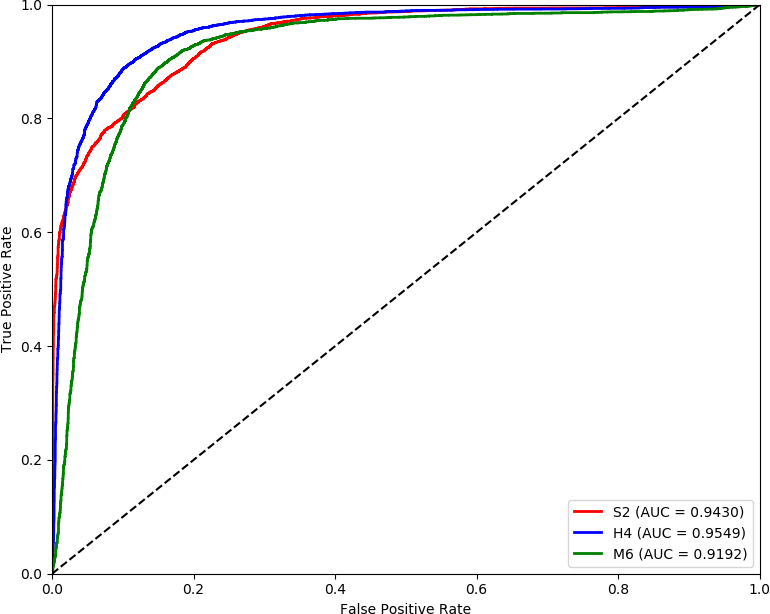
\includegraphics[width=.8\textwidth]{dados/figuras/ROC_H_10_6.png}
 \caption{Curvas ROC dos testes com o cenário H.10.6 para as CNNs treinadas com os conjuntos S2, H4 e M6 (Autoria própria).}
 \label{fig:I_Wanna_ROC!}
\end{figure}

Essa disparidade entre as métricas avaliadas pode ser explicada ao se analisar as matrizes de confusão\footnote{Matriz de confusão é uma tabela que mostra os resultados obtidos por um classificador. As linhas representam os rótulos reais, e as colunas o predito pelo classificador.} dos testes. A Tabela \ref{tab:matrix_reloaded} compara as matrizes de confusão, acurácia, precisão\footnote{Proporção de verdadeiros positivos em relação a todas predições positivas.} e revocação\footnote{Taxa de verdadeiros positivos.} obtidas pelas CNNs treinadas com os conjuntos S2 e H4 quando testados no cenário H.10.6.

\begin{table}[!htb]
\centering
\begin{tabular}{c|c|c|c|c|@{}m{0pt}@{}}
\cline{2-5}
		                          & \textbf{\begin{tabular}[c]{@{}c@{}}Matriz de\\ Confusão\end{tabular}}   & \textbf{Acurácia} & \textbf{Precisão} & \textbf{Revocação} &\\[20pt] \hline
\multicolumn{1}{|c|}{\textbf{H4}} & $\left[ \begin{array}{cc} 4156 & 844 \\ 300 & 4700 \end{array} \right]$ & 88,56\%           & 0.8477            & 0.94               &\\[21pt] \hline
\multicolumn{1}{|c|}{\textbf{S2}} & $\left[ \begin{array}{cc} 2548 & 2452 \\ 62 & 4938 \end{array} \right]$ & 74,86\%           & 0.6682            & 0.9876             &\\[21pt] \hline
\end{tabular}
\caption{Outras métricas dos testes realizados no cenário H.10.6 com as CNNs treinadas com os conjuntos H4 e S2.}
\label{tab:matrix_reloaded}
\end{table}

Também é interessante notar a baixa variação das acurácias para o \textit{payload} de 0.6 bpp, onde se tem um desvio padrão de apenas 0,093. A Tabela \ref{tab:cnn_s2} ilustra os resultados obtidos ao utilizar diferentes cenários de teste.

\begin{table}[!ht]
\centering
\begin{tabular}{c|c|c|c|c|}
\cline{2-5}
\textbf{}                             & \textbf{x = 0.1} & \textbf{x = 0.2} & \textbf{x = 0.4} & \textbf{x = 0.6} \\ \hline
\multicolumn{1}{|c|}{\textbf{H.0.x}}  & 56,1\%           & 67,59\%          & 73,59\%          & 74,76\%          \\ \hline
\multicolumn{1}{|c|}{\textbf{H.10.x}} & \textbf{57,94\%} & \textbf{69,02\%} & \textbf{73,87\%} & \textbf{74,86\%} \\ \hline
\multicolumn{1}{|c|}{\textbf{S.0.x}}  & 53,65\%          & 63,21\%          & 73,09\%          & 74,73\%          \\ \hline
\multicolumn{1}{|c|}{\textbf{S.7.x}}  & 55,03\%          & 66,78\%          & 73,65\%          & 74,83\%          \\ \hline
\multicolumn{1}{|c|}{\textbf{S.10.x}} & 54,69\%          & 65,59\%          & 73,47\%          & 74,76\%          \\ \hline
\multicolumn{1}{|c|}{\textbf{S.12.x}} & 54,3\%           & 65,36\%          & 73,45\%          & 74,79\%          \\ \hline
\multicolumn{1}{|c|}{\textbf{M.-.x}}  & 54,18\%          & 64,17\%          & 72,88\%          & 74,55\%          \\ \hline
\end{tabular}
\caption{Acurácias dos testes da CNN com o conjunto de treinamento S2.}
\label{tab:cnn_s2}
\end{table}

\subsection{Conjunto de Treinamento S4}

Os testes com a CNN treinada neste conjunto apresentaram bons resultados, ficando entre os melhores para \textit{payloads} de 0.1, 0.2 e 0.4 bpp para todos algoritmos. A Tabela \ref{tab:cnn_s4} apresenta as acurácias para todos os cenários de teste.

\begin{table}[!htb]
\centering
\begin{tabular}{c|c|c|c|c|}
\cline{2-5}
\textbf{}                             & \textbf{x = 0.1} & \textbf{x = 0.2} & \textbf{x = 0.4} & \textbf{x = 0.6} \\ \hline
\multicolumn{1}{|c|}{\textbf{H.0.x}}  & 53,78\%          & 66,74\%          & 80,25\%          & 84,43\%          \\ \hline
\multicolumn{1}{|c|}{\textbf{H.10.x}} & \textbf{55,21\%} & \textbf{69,04\%} & \textbf{81,07\%} & 84,50\%          \\ \hline
\multicolumn{1}{|c|}{\textbf{S.0.x}}  & 52,28\%          & 59,95\%          & 79,15\%          & 84,56\%          \\ \hline
\multicolumn{1}{|c|}{\textbf{S.7.x}}  & 53,08\%          & 64,30\%          & 80,94\%          & \textbf{84,89\%} \\ \hline
\multicolumn{1}{|c|}{\textbf{S.10.x}} & 52,82\%          & 62,80\%          & 80,43\%          & 84,77\%          \\ \hline
\multicolumn{1}{|c|}{\textbf{S.12.x}} & 52,64\%          & 62,39\%          & 80,00\%          & 84,65\%          \\ \hline
\multicolumn{1}{|c|}{\textbf{M.-.x}}  & 52,58\%          & 61,82\%          & 78,03\%          & 83,30\%          \\ \hline
\end{tabular}
\caption{Acurácias dos testes da CNN com o conjunto de treinamento S4.}
\label{tab:cnn_s4}
\end{table}


\subsection{Conjunto de Treinamento S6}

Este foi o conjunto de treinamento que obteve a maior acurácia para todos os cenários de teste do algoritmo S-UNIWARD com \textit{payload} de 0.6 bpp. Tendo mostrado também boa acurácia para outros algoritmos com o mesmo \textit{payload}. Porém foi um dos piores nos testes com \textit{payload} de 0.1 bpp, como pode ser visto na Tabela \ref{tab:cnn_s6}.

\begin{table}[!htb]
\centering
\begin{tabular}{c|c|c|c|c|}
\cline{2-5}
\textbf{}                             & \textbf{x = 0.1} & \textbf{x = 0.2} & \textbf{x = 0.4} & \textbf{x = 0.6} \\ \hline
\multicolumn{1}{|c|}{\textbf{H.0.x}}  & 51,12\%          & 59,21\%          & 75,72\%          & 87,01\%          \\ \hline
\multicolumn{1}{|c|}{\textbf{H.10.x}} & \textbf{51,67\%} & \textbf{61,38\%} & 77,58\%          & 87,86\%          \\ \hline
\multicolumn{1}{|c|}{\textbf{S.0.x}}  & 50,68\%          & 55,24\%          & 74,52\%          & 87,24\%          \\ \hline
\multicolumn{1}{|c|}{\textbf{S.7.x}}  & 50,98\%          & 58,51\%          & \textbf{77,67\%} & \textbf{89,12\%} \\ \hline
\multicolumn{1}{|c|}{\textbf{S.10.x}} & 50,72\%          & 57,16\%          & 76,50\%          & 88,37\%          \\ \hline
\multicolumn{1}{|c|}{\textbf{S.12.x}} & 50,81\%          & 56,80\%          & 75,89\%          & 88,12\%          \\ \hline
\multicolumn{1}{|c|}{\textbf{M.-.x}}  & 50,73\%          & 55,52\%          & 72,75\%          & 83,85\%          \\ \hline
\end{tabular}
\caption{Acurácias dos testes da CNN com o conjunto de treinamento S6.}
\label{tab:cnn_s6}
\end{table}


\subsection{Conjunto de Treinamento M1}

Este conjunto, treinado com a base contendo imagens esteganografadas com o algoritmo MiPOD, apresentou resultados medianos em todos os testes. A Tabela \ref{tab:cnn_m1} exibe as acurácias obtidas.

\begin{table}[!htb]
\centering
\begin{tabular}{c|c|c|c|c|}
\cline{2-5}
\textbf{}                             & \textbf{x = 0.1} & \textbf{x = 0.2} & \textbf{x = 0.4} & \textbf{x = 0.6} \\ \hline
\multicolumn{1}{|c|}{\textbf{H.0.x}}  & 52,87\%          & 61,84\%          & 77,76\%          & 83,15\%          \\ \hline
\multicolumn{1}{|c|}{\textbf{H.10.x}} & \textbf{53,80\%} & \textbf{64,64\%} & \textbf{79,00\%} & \textbf{83,56\%} \\ \hline
\multicolumn{1}{|c|}{\textbf{S.0.x}}  & 51,40\%          & 55,88\%          & 74,84\%          & 82,09\%          \\ \hline
\multicolumn{1}{|c|}{\textbf{S.7.x}}  & 51,98\%          & 58,11\%          & 77,29\%          & 83,08\%          \\ \hline
\multicolumn{1}{|c|}{\textbf{S.10.x}} & 51,72\%          & 57,42\%          & 76,28\%          & 82,85\%          \\ \hline
\multicolumn{1}{|c|}{\textbf{S.12.x}} & 51,65\%          & 57,07\%          & 76,02\%          & 82,63\%          \\ \hline
\multicolumn{1}{|c|}{\textbf{M.-.x}}  & 51,98\%          & 58,18\%          & 76,14\%          & 82,20\%          \\ \hline
\end{tabular}
\caption{Acurácias dos testes da CNN com o conjunto de treinamento M1.}
\label{tab:cnn_m1}
\end{table}

\subsection{Conjunto de Treinamento M2}

Assim como o conjunto S4, o M2 também ficou entre os melhores nos testes com \textit{payloads} de 0.1, 0.2, e 0.4 bpp, porém foi um dos piores nos testes com 0.6. A Tabela \ref{tab:cnn_m2} apresenta os resultados obtidos. Assim como na maioria dos testes, cenário H.10.x foi o que apresentou as maiores taxas de acurácia. 

\begin{table}[!htb]
\centering
\begin{tabular}{c|c|c|c|c|}
\cline{2-5}
\textbf{}                             & \textbf{x = 0.1} & \textbf{x = 0.2} & \textbf{x = 0.4} & \textbf{x = 0.6} \\ \hline
\multicolumn{1}{|c|}{\textbf{H.0.x}}  & 53,80\%          & 63,09\%          & 78,96\%          & 82,46\%          \\ \hline
\multicolumn{1}{|c|}{\textbf{H.10.x}} & \textbf{54,94\%} & \textbf{65,94\%} & \textbf{79,93\%} & \textbf{82,59\%} \\ \hline
\multicolumn{1}{|c|}{\textbf{S.0.x}}  & 52,25\%          & 57,86\%          & 75,74\%          & 81,92\%          \\ \hline
\multicolumn{1}{|c|}{\textbf{S.7.x}}  & 52,92\%          & 60,29\%          & 78,40\%          & 82,46\%          \\ \hline
\multicolumn{1}{|c|}{\textbf{S.10.x}} & 52,72\%          & 59,49\%          & 77,58\%          & 82,27\%          \\ \hline
\multicolumn{1}{|c|}{\textbf{S.12.x}} & 52,64\%          & 58,94\%          & 76,90\%          & 82,10\%          \\ \hline
\multicolumn{1}{|c|}{\textbf{M.-.x}}  & 52,94\%          & 60,59\%          & 77,46\%          & 82,00\%          \\ \hline
\end{tabular}
\caption{Acurácias dos testes da CNN com o conjunto de treinamento M2.}
\label{tab:cnn_m2}
\end{table}


\subsection{Conjunto de Treinamento M4}

A Tabela \ref{tab:cnn_m4} apresenta os resultados obtidos com este conjunto de treinamento, que teve boas taxas de acerto nos testes com \textit{payloads} de 0.4 e 0.6 bpp. Foi o melhor desempenho obtido em todos os testes para o cenário M.-.6, onde alcançou 85.94\% de acurácia, superando inclusive a abordagem com SRM + \textit{ensemble of classifiers}.

\begin{table}[!htb]
\centering
\begin{tabular}{c|c|c|c|c|}
\cline{2-5}
\textbf{}                             & \textbf{x = 0.1} & \textbf{x = 0.2} & \textbf{x = 0.4} & \textbf{x = 0.6} \\ \hline
\multicolumn{1}{|c|}{\textbf{H.0.x}}  & 51,61\%          & 57,49\%          & 79,67\%          & 86,44\%          \\ \hline
\multicolumn{1}{|c|}{\textbf{H.10.x}} & \textbf{52,17\%} & \textbf{60,59\%} & \textbf{81,55\%} & \textbf{87,05\%} \\ \hline
\multicolumn{1}{|c|}{\textbf{S.0.x}}  & 51,09\%          & 54,10\%          & 73,14\%          & 85,51\%          \\ \hline
\multicolumn{1}{|c|}{\textbf{S.7.x}}  & 51,36\%          & 55,54\%          & 78,52\%          & 86,48\%          \\ \hline
\multicolumn{1}{|c|}{\textbf{S.10.x}} & 51,28\%          & 54,83\%          & 76,12\%          & 86,25\%          \\ \hline
\multicolumn{1}{|c|}{\textbf{S.12.x}} & 51,24\%          & 54,73\%          & 75,43\%          & 86,08\%          \\ \hline
\multicolumn{1}{|c|}{\textbf{M.-.x}}  & 51,57\%          & 55,77\%          & 77,14\%          & 85,94\%          \\ \hline
\end{tabular}
\caption{Acurácias dos testes da CNN com o conjunto de treinamento M4.}
\label{tab:cnn_m4}
\end{table}

Observe que o desempenho para os \textit{payloads} 0.1 e 0.2 não foi bom, indicando que o treinamento para o \textit{payload} 0.4 deixa o classificador mais habilitado para identificar maiores quantidades de mensagens escondidas. Ao passo que o treinamento realizado com M1 e M2 obtém 64,64\% e 65,94\% de acurácia para o teste com \textit{payload }0.2, respectivamente, para o M4 o valor é de 60,59\%.

\subsection{Conjunto de Treinamento M6}

Os resultados do conjunto M6, mostrados na Tabela \ref{tab:cnn_m6}, foram os piores em comparação com os obtidos pelos outros conjuntos em grande parte dos testes. Apresentando resultados satisfatórios apenas quando testado com \textit{payload} de 0.6 bpp.

\begin{table}[!htb]
\centering
\begin{tabular}{c|c|c|c|c|}
\cline{2-5}
\textbf{}                             & \textbf{x = 0.1} & \textbf{x = 0.2} & \textbf{x = 0.4} & \textbf{x = 0.6} \\ \hline
\multicolumn{1}{|c|}{\textbf{H.0.x}}  & 50,52\%          & 51,86\%          & 65,65\%          & 84,16\%          \\ \hline
\multicolumn{1}{|c|}{\textbf{H.10.x}} & \textbf{50,63\%} & \textbf{52,29\%} & \textbf{69,96\%} & \textbf{86,12\%} \\ \hline
\multicolumn{1}{|c|}{\textbf{S.0.x}}  & 50,37\%          & 51,35\%          & 57,59\%          & 80,20\%          \\ \hline
\multicolumn{1}{|c|}{\textbf{S.7.x}}  & 50,45\%          & 51,63\%          & 61,46\%          & 84,46\%          \\ \hline
\multicolumn{1}{|c|}{\textbf{S.10.x}} & 50,44\%          & 51,59\%          & 59,65\%          & 82,80\%          \\ \hline
\multicolumn{1}{|c|}{\textbf{S.12.x}} & 50,39\%          & 51,60\%          & 59,30\%          & 82,28\%          \\ \hline
\multicolumn{1}{|c|}{\textbf{M.-.x}}  & 50,48\%          & 51,48\%          & 63,61\%          & 83,87\%          \\ \hline
\end{tabular}
\caption{Acurácias dos testes da CNN com o conjunto de treinamento M6.}
\label{tab:cnn_m6}
\end{table}


% \section{Detecção do LSB \textit{Matching}}
% 
% EXPLICAR AQUI PQ FOI USADA (PARA VALIDAÇÃO).
% MENCIONAR ESTADO DA ARTE (SE É VALIDAÇÃO, DEVE ESTAR COMPATÍVEL)!!!
% 
% O LSB-Matching~\citeauthorlsb_matching_revised} foi implementado em C++ pelos próprios autores desse trabalho segundo as especificações de \citeonline{sharp2001implementation} e \citeonline{lsb_matching_revised}\footnote{Disponível em: \url{https://github.com/yudi-matsuzake/stegim}.}. 
% 
% A Tabela \ref{tab:lsbespecial} mostra os resultados obtidos com cada um dos conjuntos de treinamento, quando testados com o LSB \textit{Matching}. Os resultados, 
%ESSA ARGUMENTAÇÃO NÃO ESTÁ BOA, CONFORME CONVERSAMOS!!!
%apesar de estarem não estado da arte de detecção do LSB \textit{Matching}, porém, nesse caso ele foi utilizado para apenas a validação da rede. Conforme exemplificado na Figura~\ref{fig:comp}, fica claro perceber o motivo desses resultados quando se analisa a diferença de abordagens dos algoritmos adaptativos e não-adaptativos.

% \begin{table}[!htb]
% \centering
% \caption{Acurácias da detecção do LSB \textit{Matching}.}
% \label{tab:lsbespecial}
% \begin{tabular}{c|c|c|c|c|}
% \cline{2-5}
%                                   & \textbf{0.1} & \textbf{0.2} & \textbf{0.4} & \textbf{0.6} \\ \hline
% \multicolumn{1}{|c|}{\textbf{H1}} & 53,93\%        & 65,03\%        & 83,34\%        & 86,86\%        \\ \hline
% \multicolumn{1}{|c|}{\textbf{H2}} & 53,21\%        & 63,47\%        & 86,62\%        & 89,77\%        \\ \hline
% \multicolumn{1}{|c|}{\textbf{H4}} & 54,25\%        & 70,75\%        & 89,94\%        & 91,06\%        \\ \hline
% \multicolumn{1}{|c|}{\textbf{H6}} & 52,79\%        & 68,85\%        & 91,67\%        & \textbf{95,22}\%        \\ \hline
% \multicolumn{1}{|c|}{\textbf{S1}} & 53,67\%        & 66,29\%        & 89,04\%        & 90,64\%        \\ \hline
% \multicolumn{1}{|c|}{\textbf{S2}} & \textbf{60,81}\%        & 73,75\%        & 75,19\%        & 75,37\%        \\ \hline
% \multicolumn{1}{|c|}{\textbf{S4}} & 60,51\%        & \textbf{81,84}\%        & 86,02\%        & 86,3 \%        \\ \hline
% \multicolumn{1}{|c|}{\textbf{S6}} & 57,75\%        & 79,86\%        & \textbf{93,15}\%        & 93,97\%        \\ \hline
% \multicolumn{1}{|c|}{\textbf{M1}} & 55,41\%        & 72,89\%        & 84,38\%        & 85,71\%        \\ \hline
% \multicolumn{1}{|c|}{\textbf{M2}} & 55,88\%        & 73,42\%        & 84,26\%        & 84,91\%        \\ \hline
% \multicolumn{1}{|c|}{\textbf{M4}} & 53,99\%        & 68,46\%        & 87,99\%        & 89,06\%        \\ \hline
% \multicolumn{1}{|c|}{\textbf{M6}} & 51,78\%        & 57,68\%        & 86,62\%        & 92,26\%        \\ \hline
% \end{tabular}
% \end{table}

\section{Análise dos Resultados}

Os experimentos realizados com o uso de SRM e \textit{ensemble} de classificadores revelaram que essa abordagem é inadequada para esteganálise cega, isto é, detectar a presença de uma mensagem oculta sem conhecimento prévio do algoritmo e \textit{payload} utilizados. Os resultados obtidos só foram bons quando o treinamento e teste foi feito com o mesmo algoritmo, e com uma taxa de bits por pixel igual ou parecida.

Já a CNN, apesar de não ter alcançado os mesmos valores de acurácia que o \textit{ensemble} de classificadores em esteganálise direcionada, se mostrou muito mais eficaz para esteganálise cega, especialmente quando treinada com \textit{payloads} de 0.2 e 0.4 bpp. As únicas exceções a isso são as CNNs treinadas com MiPOD e S-UNIWARD com 0.2 bpp quando testadas com \textit{payload} de 0.6 bpp, onde a acurácia obtida foi muito baixa.

Uma das primeiras hipóteses consideradas no início desse trabalho era que os kernels da CNN poderiam se aproximar dos filtros SRM. Porém, isso não pode ser confirmado com os experimentos,  uma vez que os dois detectores se comportam de forma diferente --- a CNN tendo poder de generalização maior enquanto o SRM se mostra mais especializado.

Outro comportamento pertinente ao se usar a CNN foi a obtenção de piores resultados ao se usar os \textit{payloads} de 0.1 bpp e 0.6 bpp para o treinamento. Isso provavelmente ocorre porque quanto mais extremo o \textit{payload}, mais especializada tende a ficar a rede.

É possível notar também que, nos cenários onde foi utilizado o STC, a acurácia dos detectores foi maior, tanto do SRM e \textit{ensemble} de classificadores quanto da CNN.

Como já esperado, o algoritmo com o uso do descritor SRM teve desempenho notável quando se testando com o algoritmo HUGO, principalmente pelo fato de ter sido estruturado para a esteganálise do mesmo. O que acabou sendo surpreendente é que o seu melhor desempenho é muito superior ao da CNN, diferença discrepante com relação ao resultados dos outros algoritmos. Como pode ser observado na Tabela \ref{tab:hugo_comp}, nos cenários H.0.1 e H.10.1  a diferença chegou a um máximo de 10\%.

\begin{table}[h]
\centering
\caption{Comparação entre os melhores resultados para o algoritmo HUGO com uso do SRM e com uso da CNN}
\label{tab:hugo_comp}
\begin{tabular}{|c|c|c|c|c|c|c|c|c|}
\hline
    & H.0.1   & H.0.2   & H.0.4   & H.0.6   & H.10.1  & H.10.2  & H.10.4  & H.10.6  \\ \hline
SRM & 66,23\% & 73,89\% & 84,60\% & 90,46\% & 67,02\% & 75,30\% & 85,43\% & 91,18\% \\ \hline
CNN & 56,10\% & 67,59\% & 80,25\% & 88,01\% & 57,94\% & 69,04\% & 81,55\% & 88,56\% \\ \hline
\end{tabular}
\end{table}

Apesar das acurácias diferirem bastante, principalmente para o algoritmo HUGO, as AUCs para o \textit{payload} de 0.1 bpp não tem um contraste tão evidente, como mostrado na Figura \ref{fig:ROC_H}(a), na qual a CNN chegou, inclusive, a ter a curva superior ao SRM em vários pontos. Esse mesmo comportamento não se repete para o \textit{payload} de 0.6 bpp, como pode ser visto na Figura \ref{fig:ROC_H}(b), onde a curva do SRM é sempre superior a da CNN.

\begin{figure}[!ht]
\centering
	\subfloat[HUGO 0.1]{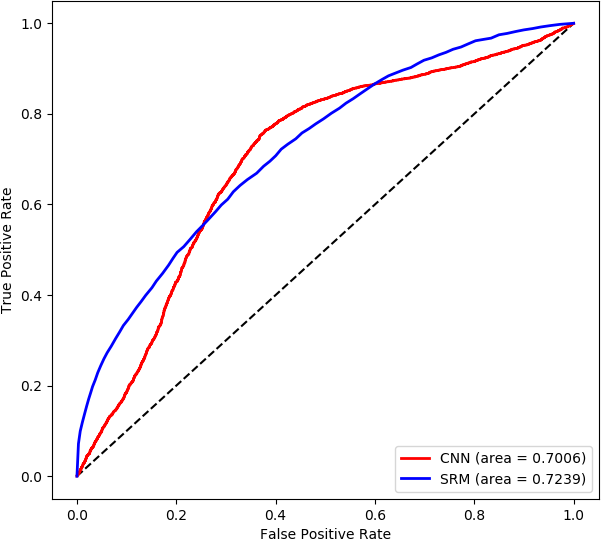
\includegraphics[width=0.45\textwidth]{dados/figuras/H1_H_0_1.png}}\;
	\subfloat[HUGO 0.6]{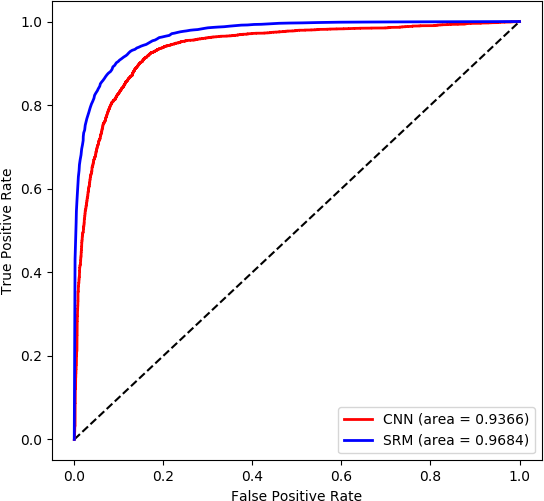
\includegraphics[width=0.45\textwidth]{dados/figuras/H6_H_0_6.png}} 
	\caption{Curvas ROC da CNN e do SRM para os cenários de teste e treino iguais (Autoria própria)}
    \label{fig:ROC_H}
\end{figure}

A Figura \ref{fig:ROC_M} ilustra um conjunto de treino no qual o SRM teve desempenho inferior à CNN em todos os cenários de teste que fazem uso do MiPOD, tanto com relação as acurácias quanto as AUCs. Isso ocorre porque o treino foi feito com um algoritmo de menor complexidade que o de teste, situação que piora consideravelmente a performance do SRM.

\begin{figure}[!htb]
 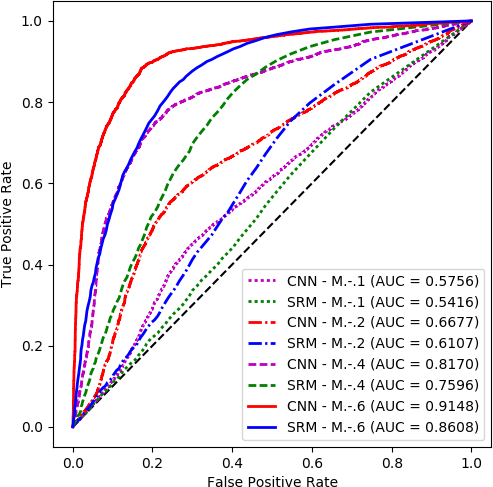
\includegraphics[width=.8\textwidth]{dados/figuras/H6_M-_x.png}
 \caption{Curvas ROC dos testes com o MiPOD e treinos com o cenário H6. (Autoria própria).}
 \label{fig:ROC_M}
\end{figure}

Uma característica em comum às duas arquiteturas foi a maior dificuldade de detectar a presença do algoritmo MiPOD. No caso do SRM, isso é ainda mais notável quando o classificador é treinado com um algoritmo diferente do MiPOD.

Com relação ao desempenho computacional, foi possível notar que o tempo de treino do \textit{ensemble} de classificadores com FLD é muito menor que o da CNN, porém o descritor SRM tem alta complexidade computacional pela quantidade de convoluções que são realizadas para cada filtro do algoritmo. Mesmo com a alta complexidade do descritor, a CNN é mais custosa computacionalmente no processo como um todo. 

Os Apêndices~\ref{chap:apendiceA} e \ref{chap:apendiceB} apresentam os valores de AUC para as duas abordagens.



% \section{Assinatura baseada em Scene Frames}

% Traduzir scene frame?

Outra abordagem, proposta por \cite{mao2015sceneframe}, é baseada na assinatura de \textit{scene frames}, ou quadros de cena. O algoritmo fundamenta-se na ideia de que as chances de existirem cinco quadros de cena seguidos é extremamente baixa. De acordo com os autores, um quadro de cena pode ser representado tanto por quadros de referência (chamados \textit{intraframes}), quanto pelos quadros que são codificados pelo mesmo (\textit{interframes}), contanto que siga duas características: o quadro deve ser uma imagem no formato espacial; e os mesmos objetos, além de um \textit{background} altamente similar, devem pertencem a uma mesma cena.

\subsection{A extração de assinatura}

Primeiramente, todo quadro é pré-processado, seguindo uma série de passos que serão descritos a seguir:

\begin{enumerate}
	\item O componente de luminância é obtido
   	\item O quadro é recortado, utilizando-se apenas sua área central
    \item O quadro é redimensionado para o tamanho de $3/4$QCIF, ou seja, $(108\times132)$
\end{enumerate}

Após o processamento inicial, o quadro é então dividido em $144$ pedaços menores, de tamanho $(9\times11)$, cuja média de intensidade irá compor parte da assinatura deste quadro. Além dos $144$ valores, o descritor é composto também por $576$ elementos diferenciais, totalizando $720$ valores. Para obter esses elementos, cada fragmento é dividido em oito elementos menores, como mostra a Figura \ref{fig:divsceneframe}, e então é realizada a subtração de $a - b$, $c - d$, $e - f$ e $g - h$.

\begin{figure}[h]
	\centering
    \label{fig:divsceneframe}
	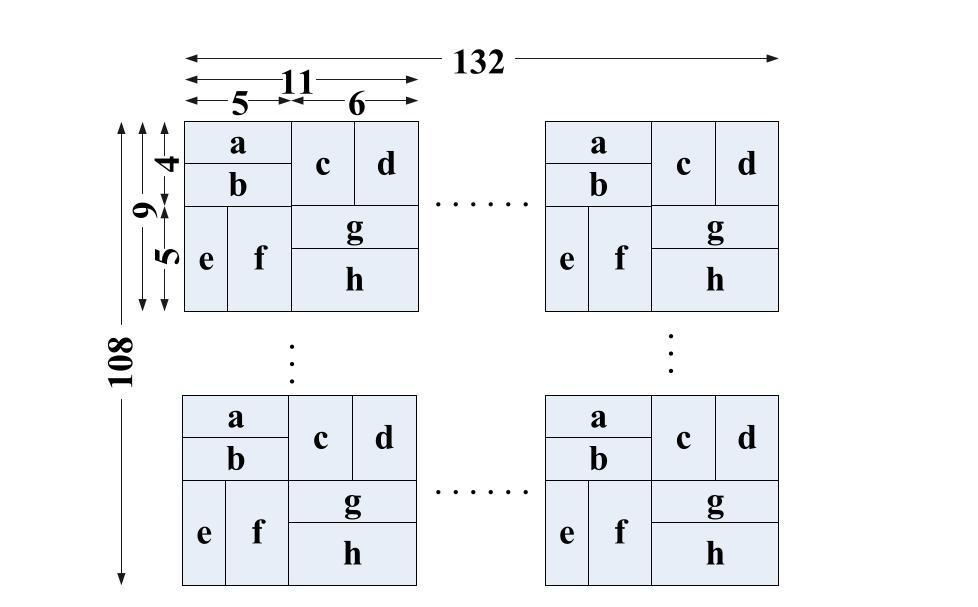
\includegraphics[width=\textwidth]{images/divisaosceneframe.jpg}
    \caption{Divisão da imagem para cálculo dos elementos diferenciais. Referência: \cite{mao2015sceneframe}}
\end{figure}

\subsection{Diminuição do espaço de memória utilizado}

O artigo também propõe uma alternativa para diminuir o espaço de memória utilizado para armazenar as assinaturas, visto que o banco de dados dos vídeos pode ser grande. Para isso, é proposta uma técnica chamada qualificação quaternária, na qual os valores são classificados de acordo com um \textit{threshold}.



                   % Scene Frame
% % RESULTADOS-------------------------------------------------------------------

\chapter{Análise e Discussão dos Resultados}
\label{chap:resultados}

Este capítulo discute os resultados obtidos nas duas abordagens de esteganálise estudadas neste trabalho. Como descrito anteriormente, a primeira é baseada no descritor SRM - posteriormente utilizado em um conjunto (\textit{ensemble}) de classificadores - e a segunda em CNNs. 

Conforme detalhado no capítulo anterior, são considerados 12 conjuntos de treinamento, resultantes da aplicação dos algoritmos de esteganografia HUGO, S-UNIWARD e MiPOD para quatro diferentes \textit{payloads}: 0.1, 0.2, 0.4 e 0.6 bpp. Visando facilitar a identificação de um conjunto específico, serão consideradas as siglas definidas na Tabela~\ref{tab:cenariosTrain}, compostas pela primeira letra do nome do algoritmo de esteganografia seguida do valor do \textit{payload} (por exemplo, H6 representa HUGO com \textit{payload} 0.6 bpp).

Além disso, também são definidos 28 conjuntos de teste, listados na Tabela~\ref{tab:cenariosTest}. Cada um deles é identificado por uma sigla composta pela primeira letra do nome do algoritmo de esteganografia utilizado para gerar a estego imagem, seguida por dois valores: um  que representa o STC e outro que identifica o \textit{payload} (por exemplo, H.0.2 representa o HUGO com STC 0 e \textit{payload} 0.2 bpp).

Cada um dos 12 conjuntos de treinamento é utilizado separadamente para treinamento das duas abordagens de esteganálise. Os modelos de classificação resultantes (\textit{ensemble} de classificadores ou CNN) são então aplicados em diferentes conjuntos de teste (x denota a variação para os quatro \textit{payloads}):
\begin{enumerate}%TODO
\item SRM + \textit{Ensemble}: sete conjuntos - H.0.x, H.10.x, S.0.x, S.10.1, S.10.4, S.10.6, M.0.x\footnote{Por limitação de tempo não foram realizados os demais testes.}.
\item CNN: todos os 28 conjuntos listados na Tabela~\ref{tab:cenariosTest} - H.0.x, H.10.x, S.0.x, S.7.x, S.10.x, S.12.x, M.-.x.
\end{enumerate}
Com isso, tem-se um total de 12 $\times$ 7 + 12 $\times$ 28 = 420 resultados.

Na sequência, serão discutidos os resultados obtidos, os quais serão divididos por abordagem de esteganálise e depois por conjunto de treinamento. Ao final, será realizada uma análise geral dos resultados. Os Apêndices \ref{chap:apendiceA} e \ref{chap:apendiceB} mostram tabelas das áreas sob a curva (AUC) obtidas nos testes com SRM e CNN respectivamente.

\clearpage
\section{Resultados com SRM e \textit{Ensemble} de Classificadores}

Em geral, o comportamento da seleção de características é semelhante para todos \textit{payloads}de 1000 à 1400 características. No caso do número de classificadores, os dois \textit{payloads} menores variam de 70 à 80 enquanto os maiores variam de 90 à 100. Tais comportamentos são ilustrado na Figura \ref{fig:srm_train}, para o caso do conjunto de treinamento M1.

\begin{figure}[ht]
\centering
	\subfloat[]{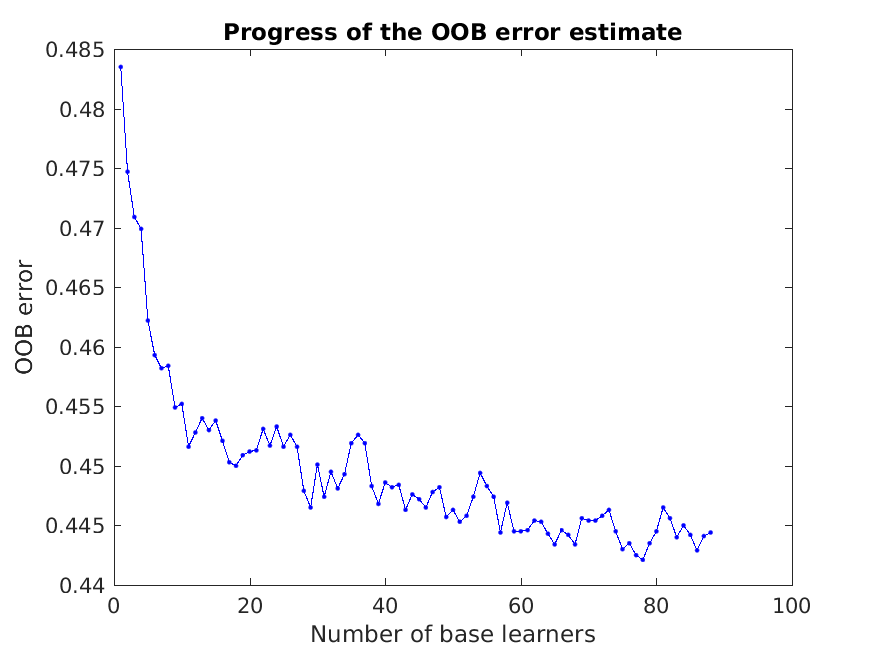
\includegraphics[width=0.7\textwidth]{dados/figuras/oob.png}}\qquad
	\subfloat[]{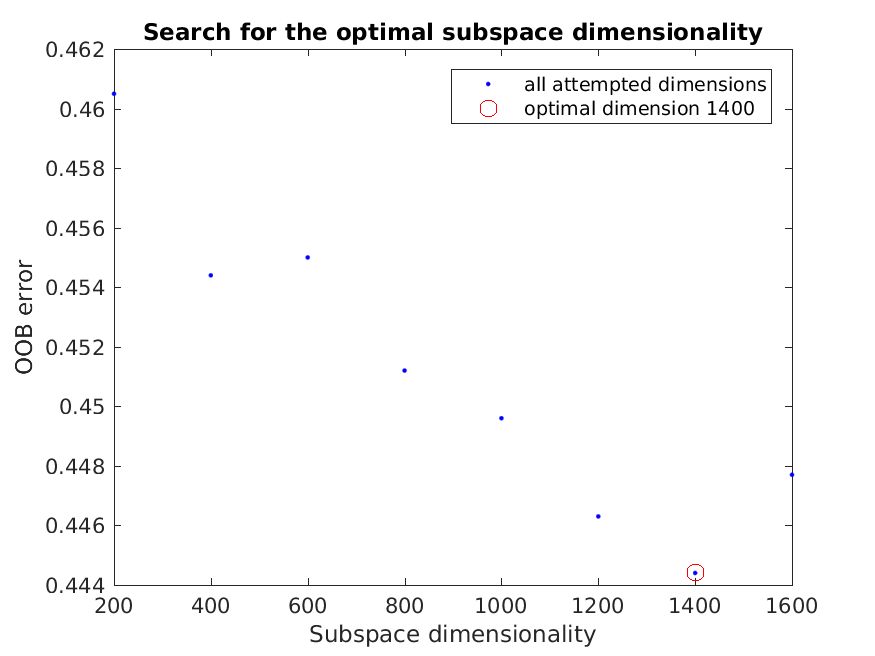
\includegraphics[width=0.7\textwidth]{dados/figuras/dimesion.png}}\\ 

\caption{(a) Variação do OOBe com relação ao número de classificadores para o cojunto de treinamento M1. (b) Variação do OOBe com relação ao número de características para o conjunto de treinamento M1 (Autoria própria).}
\label{fig:srm_train}
\end{figure}

Outro fato interessante é o comportamento dos classificadores base para os diferentes \textit{payloads} de teste. A Figura \ref{fig:votes}(a) mostra a assertividade quando o \textit{payload} de treinamento e teste são próximos, dado que existe uma tendência do indicador estar próximo da extremidade e com os tipos de imagens, estego ou cobertura, na posição desejada.

Além disso, quando o classificador treinado em um conjunto de treinamento com  \textit{payload} alto é aplicado em um conjunto de testes que possui \textit{payload} baixo, o histograma tende a estar mais elevado para a esquerda tanto para as imagens de cobertura quanto para as estego imagens. Isso ocorre porque, como o \textit{payload} de teste é muito menor que o de treino, a rede confunde quase todas as imagens com imagens de cobertura. Esse comportamento é recíproco para \textit{payloads} de treino e teste inversos, porém a confusão ocorre com estego imagens (um exemplo pode ser visto na Figura \ref{fig:votes}(b)).

\begin{figure}[!htb]
\centering
	\subfloat[]{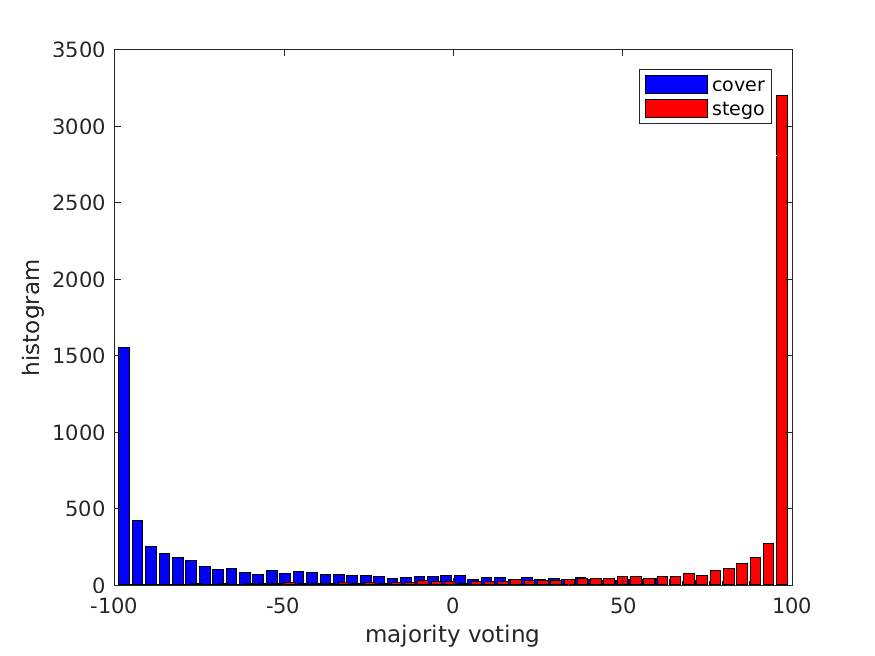
\includegraphics[width=0.45\textwidth]{dados/figuras/voting2.png}}\qquad
	\subfloat[]{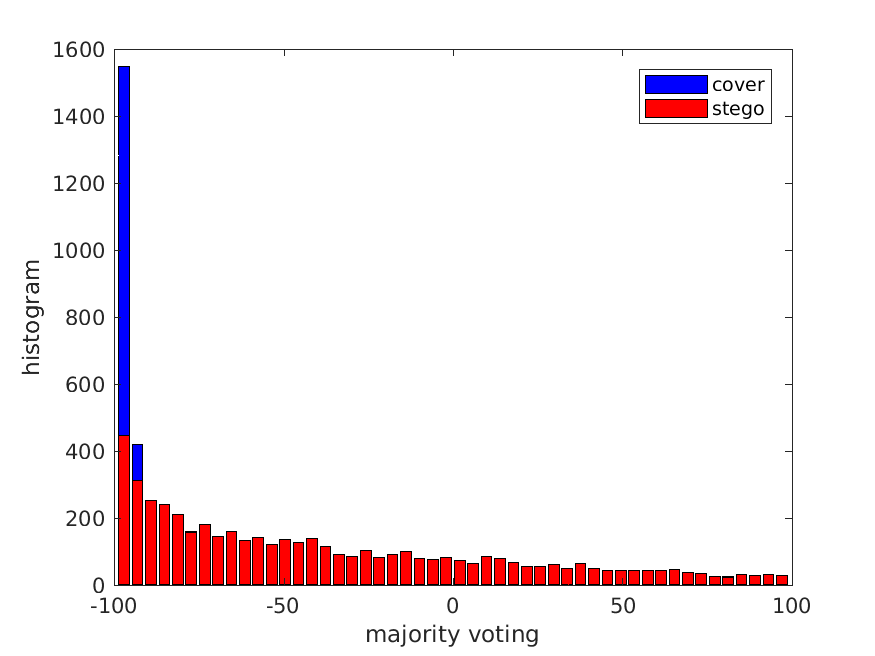
\includegraphics[width=0.45\textwidth]{dados/figuras/voting3.png}}\\ 

\caption{(a) Histograma de votação para o conjunto de treino H4 e de teste H.0.6. (b) Histograma de votação para o conjunto de treino H6 e de teste H.0.1. (Autoria própria)}
\label{fig:votes}
\end{figure}





As seções a seguir apresentarão os resultados da classificação das imagens com o uso do descritor SRM para os 12 diferentes conjuntos de treino.

\clearpage
\subsection{Conjunto de Treinamento H1}

Os resultados para o conjunto de treinamento H1 podem ser vistos na Tabela \ref{tab:srm_h1}. Os melhores resultados foram obtidos com o \textit{payload} de teste igual ao de treino e resultados inferiores nos demais cenários de teste. Essas situações mostram as principais características observadas ao se usar o descritor SRM com \textit{ensemble} de classificadores: melhores performances quando se usando \textit{payload} próximo e mesmo algoritmo de treino e teste, baixa performance ao testar com \textit{payloads} muito distintos do de teste, além da facilidade na detecção do algoritmo HUGO em relação aos outros dois algoritmos.

\begin{table}[!htb]
\centering
\begin{tabular}{c|c|c|c|c|}
\cline{2-5}
\textbf{}                             & \textbf{x = 0.1} & \textbf{x = 0.2} & \textbf{x = 0.4} & \textbf{x = 0.6} \\ \hline
\multicolumn{1}{|c|}{\textbf{H.0.x}}  & 66,23\%          & 72,48\%          & 77,57\%          & 79,31\%          \\ \hline
\multicolumn{1}{|c|}{\textbf{H.10.x}} & \textbf{67,02\%} & \textbf{73,25\%} & \textbf{77,79\%} & \textbf{79,42\%} \\ \hline
\multicolumn{1}{|c|}{\textbf{S.0.x}}  & 58,78\%          & 66,91\%          & 74,68\%          & 78,11\%          \\ \hline
\multicolumn{1}{|c|}{\textbf{S.10.x}} & 59,78\%          & 67,71\%         & 75,20\%          & 78,24\%          \\ \hline
\multicolumn{1}{|c|}{\textbf{M.-.x}}  & 57,86\%          & 64,77\%          & 71,92\%          & 75,61\%          \\ \hline
\end{tabular}
\caption{Acurácias dos testes do SRM com o conjunto de treinamento H1.}
\label{tab:srm_h1}
\end{table}


\subsection{Conjunto de Treinamento H2}

Do mesmo modo que para o conjunto de treino anterior, os melhores resultados foram obtidos para os cenários de teste com uso do HUGO. Porém, os resultados para os conjuntos H.0.4, H.0.6, H.10.4, H.10.6 foram muito superiores. Os resultados podem ser vistos na Tabela \ref{tab:srm_h2}.

\begin{table}[!htb]
\centering
\begin{tabular}{c|c|c|c|c|}
\cline{2-5}
\textbf{}                             & \textbf{x = 0.1} & \textbf{x = 0.2} & \textbf{x = 0.4} & \textbf{x = 0.6} \\ \hline
\multicolumn{1}{|c|}{\textbf{H.0.x}}  & 63,24\%          & 73,89\%    & 82,23\%          & 84,47\%          \\ \hline
\multicolumn{1}{|c|}{\textbf{H.10.x}} & \textbf{65,03\%} & \textbf{75,30\%} & \textbf{82,70\%} & \textbf{84,69\%} \\ \hline
\multicolumn{1}{|c|}{\textbf{S.0.x}}  & 52,83\%          & 64,02\%          & 77,11\%          & 82,51\%          \\ \hline
\multicolumn{1}{|c|}{\textbf{S.10.x}} & 53,95\%          & 65,86\%          & 78,22\%          & 82,89\%          \\ \hline
\multicolumn{1}{|c|}{\textbf{M.-.x}}  & 52,70\%          & 61,50\%          & 73,73\%          & 79,95\%          \\ \hline
\end{tabular}
\caption{Acurácias dos testes do SRM com o conjunto de treinamento H2.}
\label{tab:srm_h2}
\end{table}


\subsection{Conjunto de Treinamento H4}

A Tabela \ref{tab:srm_h4} mostra que o conjunto apresentou, como esperado, os melhores resultados para o algoritmo HUGO com o \textit{payload} de 0.4 bpp e valores acima de 89\% para os cenários H.10.6 e H.0.6, os quais só não superaram o conjunto de treino H6.

\begin{table}[!htb]
\centering
\begin{tabular}{c|c|c|c|c|}
\cline{2-5}
\textbf{}                             & \textbf{x = 0.1} & \textbf{x = 0.2} & \textbf{x = 0.4} & \textbf{x = 0.6} \\ \hline
\multicolumn{1}{|c|}{\textbf{H.0.x}}  & 53,55\%          & 60,80\%          & 84,60\%          & 89,11\%          \\ \hline
\multicolumn{1}{|c|}{\textbf{H.10.x}} & \textbf{54,85\%} & \textbf{70,39\%} & \textbf{85,43\%} & \textbf{89,36\%} \\ \hline
\multicolumn{1}{|c|}{\textbf{S.0.x}}  & 50,75\%          & 53,75\%          & 73,42\%          & 84,48\%          \\ \hline
\multicolumn{1}{|c|}{\textbf{S.10.x}} & 51,04\%          & 55,46\%         & 75,67\%          & 85,36\%          \\ \hline
\multicolumn{1}{|c|}{\textbf{M.-.x}}  & 50,78\%          & 52,90\%          & 68,50\%          & 80,17\%          \\ \hline
\end{tabular}
\caption{Acurácias dos testes do SRM com o conjunto de treinamento H4}
\label{tab:srm_h4}
\end{table}


\subsection{Conjunto de Treinamento H6}

Nos experimentos, o conjunto de treinamento H6 obteve os melhores resultados para os cenários H.10.6 e H.0.6 com 91,81\% e 90,46\% de acurácia respectivamente. Os resultados podem ser vistos na Tabela~\ref{tab:srm_h6}.

\begin{table}[!htb]
\centering
\begin{tabular}{c|c|c|c|c|}
\cline{2-5}
\textbf{}                             & \textbf{x = 0.1} & \textbf{x = 0.2} & \textbf{x = 0.4} & \textbf{x = 0.6} \\ \hline
\multicolumn{1}{|c|}{\textbf{H.0.x}}  & 51,13\%          & 58,98\%          & \textbf{81,30\%}          & 90,46\%          \\ \hline
\multicolumn{1}{|c|}{\textbf{H.10.x}} & \textbf{51,46\%} & \textbf{61,14\%} & 77,79\% & \textbf{91,18\%} \\ \hline
\multicolumn{1}{|c|}{\textbf{S.0.x}}  & 50,41\%          & 51,64\%          & 64,44\%          & 79,46\%          \\ \hline
\multicolumn{1}{|c|}{\textbf{S.10.x}} & 50,46\%          & 51,94\%         & 66,66\%          & 81,52\%          \\ \hline
\multicolumn{1}{|c|}{\textbf{M.-.x}}  & 50,38\%          & 51,28\%          & 60,05\%          & 73,73\%          \\ \hline
\end{tabular}
\caption{Acurácias dos testes do SRM com o conjunto de treinamento H6.}
\label{tab:srm_h6}
\end{table}


\subsection{Conjunto de Treinamento S1}

Todos os melhores resultados para o algoritmo S-UNIWARD foram obtidos com os conjuntos treinados com o mesmo algoritmo e mesmo \textit{payload}. No caso do S1, a Tabela \ref{tab:suni_s1} mostra que foram obtidas acurácias interessantes para os cenários H.0.1, H.10.1, S.0.1, S.10.1 e M.1, mesmo que com acurácia muito abaixo da obtida pelos conjuntos treinados e testados com o HUGO para o mesmo \textit{payload}.

\begin{table}[!htb]
\centering
\begin{tabular}{c|c|c|c|c|}
\cline{2-5}
\textbf{}                             & \textbf{x = 0.1} & \textbf{x = 0.2} & \textbf{x = 0.4} & \textbf{x = 0.6} \\ \hline
\multicolumn{1}{|c|}{\textbf{H.0.x}}  & 59,54\%          & 66,68\%          & 74,59\%          & 79,54\%          \\ \hline
\multicolumn{1}{|c|}{\textbf{H.10.x}} & 61,19\%          & 66,43\%          & 75,22\%          & 78,76\%   \\ \hline
\multicolumn{1}{|c|}{\textbf{S.0.x}}  & \textbf{61,53\%}          & \textbf{69,97\%}          & 77,10\%          & \textbf{79,87\%}          \\ \hline
\multicolumn{1}{|c|}{\textbf{S.10.x}} &
61,09\% & 69,75\% & \textbf{77,46\%} & 80,22\% \\ \hline
\multicolumn{1}{|c|}{\textbf{M.-.x}}  & 59,85\%          & 66,06\%          & 73,50\%          & 77,28\%          \\ \hline
\end{tabular}
\caption{Acurácias dos testes do SRM com o conjunto de treinamento S1.}
\label{tab:suni_s1}

\end{table}



\subsection{Conjunto de Treinamento S2}

A Tabela \ref{tab:suni_s2} apresenta os resultados para o conjunto de treino S2. Como já dito anteriormente, o conjunto obteve os melhores resultados para o cenário S.0.2, além de resultados bons para o \textit{payload} de 0.4 bpp.
\begin{table}[!htb]
\centering
\begin{tabular}{c|c|c|c|c|}
\cline{2-5}
\textbf{}                             & \textbf{x = 0.1} & \textbf{x = 0.2} & \textbf{x = 0.4} & \textbf{x = 0.6} \\ \hline
\multicolumn{1}{|c|}{\textbf{H.0.x}}  & 58,65\%          & 69,30\%          & 79,94\%          & 84,37\%          \\ \hline
\multicolumn{1}{|c|}{\textbf{H.10.x}} & 59,67\% & 69,50\% & 79,63\% & 83,82\% \\ \hline
\multicolumn{1}{|c|}{\textbf{S.0.x}}  & 59,20\%          & \textbf{70,40\%}          & 81,24\%         & \textbf{84,90\%}          \\ \hline
\multicolumn{1}{|c|}{\textbf{S.10.x}} & \textbf{60,59\%}          & 71,49\%
& \textbf{82,01\%}          & 84,99\%          \\ \hline
\multicolumn{1}{|c|}{\textbf{M.-.x}}  & 57,60\%          & 66,79\%          & 76,84\%          & 82,05\%          \\ \hline
\end{tabular}
\caption{Acurácias dos testes do SRM com o conjunto de treinamento S2.}
\label{tab:suni_s2}

\end{table}



\subsection{Conjunto de Treinamento S4}

A única exceção a regra, o conjunto S4 obteve tanto os melhores resultados dentre todos os conjuntos de treino tanto para o cenário S.0.4 quanto para o S.0.6. Seus resultados podem ser vistos na Tabela \ref{tab:suni_s4}.

\begin{table}[!htb]
\centering
\begin{tabular}{c|c|c|c|c|}
\cline{2-5}
\textbf{}                             & \textbf{x = 0.1} & \textbf{x = 0.2} & \textbf{x = 0.4} & \textbf{x = 0.6} \\ \hline
\multicolumn{1}{|c|}{\textbf{H.0.x}}  & 53,98\%          & 65,23\%          & 79,86\%          & 88,17\%          \\ \hline
\multicolumn{1}{|c|}{\textbf{H.10.x}} & \textbf{55,33\%} & \textbf{66,08\%} & 81,29\% & 87,86\% \\ \hline
\multicolumn{1}{|c|}{\textbf{S.0.x}}  & 52,81\%          & 64,08\%          & 81,89\%          & \textbf{89,64\%}          \\ \hline
\multicolumn{1}{|c|}{\textbf{S.10.x}} & 53,68\%          & 66,31\%          & \textbf{83,31}\%          & 88,95\%          \\ \hline
\multicolumn{1}{|c|}{\textbf{M.-.x}}  & 52,42\%          & 61,86\%          & 77,99\%          & 85,34\%          \\ \hline
\end{tabular}
\caption{Acurácias dos testes do SRM com o conjunto de treinamento S4.}
\label{tab:suni_s4}

\end{table}

Em comparação ao conjunto S2, os resultados para o \textit{payload} 0.1 foram significativamente melhores, enquanto que o desempenho para o \textit{payload} 0.6 aumentou. Isso sugere que a capacidade do classificador ao ser treinado com 0.4 o torna mais robusto a maiores alterações na imagem, mas prejudica os casos em que há pouca alteração.

\subsection{Conjunto de Treinamento S6}

O pior dos conjuntos de treino com o algoritmo S-UNIWARD, só obteve resultados satisfatórios para os cenários de teste H.0.6, H.10.6, S.0.6 e M.6. Os resultados para o conjunto de treino S6 podem ser vistos na Tabela \ref{tab:suni_s6}. 
\begin{table}[!htb]
\centering
\begin{tabular}{c|c|c|c|c|}
\cline{2-5}
\textbf{}                             & \textbf{x = 0.1} & \textbf{x = 0.2} & \textbf{x = 0.4} & \textbf{x = 0.6} \\ \hline
\multicolumn{1}{|c|}{\textbf{H.0.x}}  & 51,50\%          & 58,89\%          & 76,08\%          & 87,21\%          \\ \hline
\multicolumn{1}{|c|}{\textbf{H.10.x}} & \textbf{51,86\%} & \textbf{59,80\%} & 78,94\% & 88,31\% \\ \hline
\multicolumn{1}{|c|}{\textbf{S.0.x}}  & 51,12\%          & 56,29\%          & 76,67\%          & \textbf{88,93\%}          \\ \hline
\multicolumn{1}{|c|}{\textbf{S.10.x}} & 51,27\%          & 58,51\%          & \textbf{78,98\%}          & 89,71\%          \\ \hline
\multicolumn{1}{|c|}{\textbf{M.-.x}}  & 50,98\%          & 55,92\%          & 72,69\%          & 84,05\%          \\ \hline
\end{tabular}
\caption{Acurácias dos testes do SRM com o conjunto de treinamento S6.}
\label{tab:suni_s6}

\end{table}



\subsection{Conjunto de Treinamento M1}

Conforme observado na Tabela \ref{tab:srm_m1}, assim como em outros algoritmos listados na Tabelas \ref{tab:srm_m2}, \ref{tab:srm_m4}  e \ref{tab:srm_m6}, o MiPOD também é sensível a cenários de teste que fazem uso de outro algoritmo no treinamento.

A Tabela \ref{tab:srm_m1} por exemplo mostra a melhor acurácia para o cenário M.1, 61,17\%. Em compensação os resultados para todos os outros \textit{payloads} foram ruins.

\begin{table}[!htb] 
\centering
\begin{tabular}{c|c|c|c|c|}
\cline{2-5}
\textbf{}                             & \textbf{x = 0.1} & \textbf{x = 0.2} & \textbf{x = 0.4} & \textbf{x = 0.6} \\ \hline
\multicolumn{1}{|c|}{\textbf{H.0.x}}  & 60,02\%          & 66,74\%          & 74,31\%          & 78,09\%          \\ \hline
\multicolumn{1}{|c|}{\textbf{H.10.x}} & \textbf{61,65\%} & 66,88\% & 74,78\% & 79,29\% \\ \hline
\multicolumn{1}{|c|}{\textbf{S.0.x}}  & 60,94\%          & \textbf{67,93\%}          & 76,36\%          & \textbf{79,42\%}          \\ \hline
\multicolumn{1}{|c|}{\textbf{S.10.x}} & 61,49\%          & 69,38\%        & \textbf{76,69\%}          & 79,55\%          \\ \hline
\multicolumn{1}{|c|}{\textbf{M.-.x}}  & 61,17\%          & 66,65\%          & 73,55\%          & 77,41\%          \\ \hline
\end{tabular}
\caption{Acurácias dos testes do SRM com o conjunto de treinamento M1.}
\label{tab:srm_m1}

\end{table}


\subsection{Conjunto de Treinamento M2}

Curiosamente, assim como no conjunto M1, os melhores resultados, com exceção do \textit{payload} de 0.1 bpp foram obtidos utilizando o algoritmo S-UNIWARD para testes. O melhor resultado para o cenário M.2 foi com esse conjunto.
Os resultados podem ser observados na Tabela \ref{tab:srm_m2}.

\begin{table}[!htb]
\centering
\begin{tabular}{c|c|c|c|c|}
\cline{2-5}
\textbf{}                             & \textbf{x = 0.1} & \textbf{x = 0.2} & \textbf{x = 0.4} & \textbf{x = 0.6} \\ \hline
\multicolumn{1}{|c|}{\textbf{H.0.x}}  & 59,91\%          & 68,41\%          & 77,63\%          & 81,99\%          \\ \hline
\multicolumn{1}{|c|}{\textbf{H.10.x}} & \textbf{61,03\%} & 68,94\% & 78,29\% & 82,22\% \\ \hline
\multicolumn{1}{|c|}{\textbf{S.0.x}}  & 59,14\%          & \textbf{69,22\%}          & 79,14\%          & \textbf{82,90\%}          \\ \hline
\multicolumn{1}{|c|}{\textbf{S.10.x}} & 60,49\%          & 70,22\%          & \textbf{79,96\%}          & 83,11\%          \\ \hline
\multicolumn{1}{|c|}{\textbf{M.-.x}}  & 58,85\%          & 67,91\%          & 76,87\%          & 81,44\%          \\ \hline
\end{tabular}
\caption{Acurácias dos testes do SRM com o conjunto de treinamento M2.}
\label{tab:srm_m2}
\end{table}

\subsection{Conjunto de Treinamento M4}

A Tabela \ref{tab:srm_m4} mostra os resultados para o conjunto de treinamento M4, que não teve nenhum resultado muito interessante além do melhor resultado para o conjunto M.-.4.

\begin{table}[!htb]
\centering
\begin{tabular}{c|c|c|c|c|}
\cline{2-5}
\textbf{}                             & \textbf{x = 0.1} & \textbf{x = 0.2} & \textbf{x = 0.4} & \textbf{x = 0.6} \\ \hline
\multicolumn{1}{|c|}{\textbf{H.0.x}}  & 54,06\%          & 65,47\%          & 79,80\%          & 85,64\%          \\ \hline
\multicolumn{1}{|c|}{\textbf{H.10.x}} & \textbf{55,20\%} & \textbf{66,45\%} & 80,66\% & 86,27\% \\ \hline
\multicolumn{1}{|c|}{\textbf{S.0.x}}  & 52,50\%          & 63,31\%          & 80,50\%          & \textbf{86,57\%}          \\ \hline
\multicolumn{1}{|c|}{\textbf{S.10.x}} & 53,33\%          & 65,29\%          & \textbf{81,68\%}          & 87,03\%          \\ \hline
\multicolumn{1}{|c|}{\textbf{M.-.x}}  & 52,58\%          & 62,96\%          & 78,31\%          & 85,04\%          \\ \hline
\end{tabular}
\caption{Acurácias dos testes do SRM com o conjunto de treinamento M4.}
\label{tab:srm_m4}

\end{table}


\subsection{Conjunto de Treinamento M6}

O conjunto M6 tem comportamento semelhante ao conjunto anterior, com a exceção de que possui o melhor resultado para o conjunto de teste M.-.6. Os resultados estão dispostos na Tabela \ref{tab:srm_m6}.

\begin{table}[!htb]
\centering
\begin{tabular}{c|c|c|c|c|}
\cline{2-5}
\textbf{}                             & \textbf{x = 0.1} & \textbf{x = 0.2} & \textbf{x = 0.4} & \textbf{x = 0.6} \\ \hline
\multicolumn{1}{|c|}{\textbf{H.0.x}}  & 51,11\%          & 57,29\%          & 76,52\%          & 86,59\%          \\ \hline
\multicolumn{1}{|c|}{\textbf{H.10.x}} & \textbf{51,42\%} & \textbf{59,04\%} & \textbf{78,25\%} & \textbf{87,60\%} \\ \hline
\multicolumn{1}{|c|}{\textbf{S.0.x}}  & 50,75\%          & 53,82\%          & 73,91\%          & 87,17\%          \\ \hline
\multicolumn{1}{|c|}{\textbf{S.10.x}} & 51,11\%          & 54,88\%         & 76,73\%          & 88,19\%          \\ \hline
\multicolumn{1}{|c|}{\textbf{M.-.x}}  & 51,11\%          & 54,35\%          & 74,60\%          & 85,91\%          \\ \hline
\end{tabular}
\caption{Acurácias dos testes do SRM com o conjunto de treinamento M6.}
\label{tab:srm_m6}

\end{table}



\section{Resultados com CNN}

Como descrito anteriormente, as CNNs treinadas com cada um dos 12 conjuntos de treinamento são utilizadas para classificação de todas as 28 bases de teste. Para a maioria dos conjuntos os melhores resultados foram obtidos nos testes com o algoritmo HUGO com STC de altura 10. As CNNs treinadas para \textit{payloads} de 0.2 e 0.4 bpp apresentaram uma boa capacidade de generalização. Enquanto as treinadas com os demais \textit{payloads} se mostraram mais especializadas.

Nas seções a seguir são mostrados os resultados obtidos com cada conjunto de treinamento. 


\subsection{Conjunto de Treinamento H1}

Os resultados obtidos com o conjunto de treinamento H1, ou seja, aquele onde foi utilizado o algoritmo HUGO com \textit{payload} de 0.1 bpp, pode ser visto na Tabela \ref{tab:cnn_h1}. Mostrou resultados satisfatórios apenas quando testado em bases com o mesmo algoritmo usado no treinamento, especialmente nos cenários H.0.1 e H.10.1, onde apresentou a segunda maior taxa de acertos entre todas as CNNs.

\begin{table}[!htb]
\centering
\begin{tabular}{c|c|c|c|c|}
\cline{2-5}
\textbf{}                             & \textbf{x = 0.1} & \textbf{x = 0.2} & \textbf{x = 0.4} & \textbf{x = 0.6} \\ \hline
\multicolumn{1}{|c|}{\textbf{H.0.x}}  & 54,74\%          & 63,72\%          & 77,68\%          & 83,97\%          \\ \hline
\multicolumn{1}{|c|}{\textbf{H.10.x}} & \textbf{56,61\%} & \textbf{66,96\%} & \textbf{79,74\%} & \textbf{84,86\%} \\ \hline
\multicolumn{1}{|c|}{\textbf{S.0.x}}  & 51,49\%          & 55,68\%          & 70,62\%          & 81,53\%          \\ \hline
\multicolumn{1}{|c|}{\textbf{S.7.x}}  & 52,15\%          & 57,70\%          & 74,29\%          & 82,93\%          \\ \hline
\multicolumn{1}{|c|}{\textbf{S.10.x}} & 52,01\%          & 57,07\%          & 72,87\%          & 82,31\%          \\ \hline
\multicolumn{1}{|c|}{\textbf{S.12.x}} & 51,96\%          & 56,90\%          & 72,07\%          & 82,35\%          \\ \hline
\multicolumn{1}{|c|}{\textbf{M.-.x}}  & 51,99\%          & 57,81\%          & 72,76\%          & 81,76\%          \\ \hline
\end{tabular}
\caption{Acurácias dos testes da CNN com o conjunto de treinamento H1.}
\label{tab:cnn_h1}
\end{table}


\subsection{Conjunto de Treinamento H2}

Assim como o anterior, este conjunto também apresentou melhores acurácias nos testes com o algoritmo HUGO. Fato que já era esperado, visto que este é o algoritmo mais simples dos testados, além de ser o usado no treinamento desta CNN. A Tabela \ref{tab:cnn_h2} expõe os resultados dos testes.

Apesar da acurácia obtida nos cenários de teste H.0.1 e H.10.1 ser inferior àquela alcançada pelo conjunto de treinamento H1, a área sob a curva (AUC) foi superior. Tendo sido, dentre os 12 conjuntos de treinamento, a maior para esses cenários nos testes com CNN.

%TODO: COLOCAR TABELA COM AUCs

\begin{table}[!htb]
\centering
\begin{tabular}{c|c|c|c|c|}
\cline{2-5}
\textbf{}                             & \textbf{x = 0.1} & \textbf{x = 0.2} & \textbf{x = 0.4} & \textbf{x = 0.6} \\ \hline
\multicolumn{1}{|c|}{\textbf{H.0.x}}  & 52,44\%          & 60,17\%          & 78,25\%          & 86,64\%          \\ \hline
\multicolumn{1}{|c|}{\textbf{H.10.x}} & \textbf{53,80\%} & \textbf{63,53\%} & \textbf{80,96\%} & \textbf{87,38\%} \\ \hline
\multicolumn{1}{|c|}{\textbf{S.0.x}}  & 50,96\%          & 53,62\%          & 68,92\%          & 84,03\%          \\ \hline
\multicolumn{1}{|c|}{\textbf{S.7.x}}  & 51,22\%          & 55,18\%          & 73,30\%          & 85,76\%          \\ \hline
\multicolumn{1}{|c|}{\textbf{S.10.x}} & 51,10\%          & 54,58\%          & 71,56\%          & 85,07\%          \\ \hline
\multicolumn{1}{|c|}{\textbf{S.12.x}} & 51,10\%          & 54,36\%          & 70,51\%          & 84,85\%          \\ \hline
\multicolumn{1}{|c|}{\textbf{M.-.x}}  & 51,11\%          & 55,27\%          & 71,93\%          & 84,11\%          \\ \hline
\end{tabular}
\caption{Acurácias dos testes da CNN com o conjunto de treinamento H2.}
\label{tab:cnn_h2}
\end{table}


\subsection{Conjunto de Treinamento H4}

Entre todos os conjuntos, este foi o que apresentou as melhores acurácias nos testes com os cenários H.0.4, H.10.4, H.0.6 e H.10.6, isto é, com o algoritmo HUGO e \textit{payloads} de 0.4 e 0.6 bpp. Também conseguindo bons resultados nos outros algoritmos com esses \textit{payloads}, como pode ser visto na Tabela \ref{tab:cnn_h4}.

\begin{table}[!htb]
\centering
\begin{tabular}{c|c|c|c|c|}
\cline{2-5}
\textbf{}                             & \textbf{x = 0.1} & \textbf{x = 0.2} & \textbf{x = 0.4} & \textbf{x = 0.6} \\ \hline
\multicolumn{1}{|c|}{\textbf{H.0.x}}  & 52,27\%          & 60,82\%          & 80,78\%          & 88,01\%          \\ \hline
\multicolumn{1}{|c|}{\textbf{H.10.x}} & \textbf{53,29\%} & \textbf{64,23\%} & \textbf{82,63\%} & \textbf{88,56\%} \\ \hline
\multicolumn{1}{|c|}{\textbf{S.0.x}}  & 50,76\%          & 53,80\%          & 73,99\%          & 86,73\%          \\ \hline
\multicolumn{1}{|c|}{\textbf{S.7.x}}  & 51,18\%          & 55,69\%          & 78,30\%          & 87,80\%          \\ \hline
\multicolumn{1}{|c|}{\textbf{S.10.x}} & 51,07\%          & 54,80\%          & 77,04\%          & 87,33\%          \\ \hline
\multicolumn{1}{|c|}{\textbf{S.12.x}} & 50,98\%          & 54,51\%          & 75,78\%          & 87,23\%          \\ \hline
\multicolumn{1}{|c|}{\textbf{M.-.x}}  & 50,96\%          & 55,16\%          & 75,15\%          & 85,50\%          \\ \hline
\end{tabular}
\caption{Acurácias dos testes da CNN com o conjunto de treinamento H4.}
\label{tab:cnn_h4}
\end{table}


\subsection{Conjunto de Treinamento H6}

A Tabela \ref{tab:cnn_h6} ilustra os resultados do conjunto de treinamento H6, que foi um dos piores nos testes realizados, tendo atingido acurácia de apenas 51.03\% para \textit{payload} de 0.1 bpp. Contudo a AUC para esses casos ficou entre as maiores obtidas, ficando acima de 0,5648.

%TODO: AUC!

\begin{table}[!htb]
\centering
\begin{tabular}{c|c|c|c|c|}
\cline{2-5}
\textbf{}                             & \textbf{x = 0.1} & \textbf{x = 0.2} & \textbf{x = 0.4} & \textbf{x = 0.6} \\ \hline
\multicolumn{1}{|c|}{\textbf{H.0.x}}  & 50,77\%          & 56,26\%          & 73,51\%          & 85,50\%          \\ \hline
\multicolumn{1}{|c|}{\textbf{H.10.x}} & \textbf{51,03\%} & \textbf{58,68\%} & \textbf{76,02\%} & \textbf{87,11\%} \\ \hline
\multicolumn{1}{|c|}{\textbf{S.0.x}}  & 50,32\%          & 51,87\%          & 69,10\%          & 83,14\%          \\ \hline
\multicolumn{1}{|c|}{\textbf{S.7.x}}  & 50,44\%          & 53,21\%          & 72,62\%          & 86,16\%          \\ \hline
\multicolumn{1}{|c|}{\textbf{S.10.x}} & 50,38\%          & 52,74\%          & 71,38\%          & 84,67\%          \\ \hline
\multicolumn{1}{|c|}{\textbf{S.12.x}} & 50,38\%          & 52,48\%          & 70,58\%          & 84,43\%          \\ \hline
\multicolumn{1}{|c|}{\textbf{M.-.x}}  & 50,39\%          & 53,06\%          & 70,28\%          & 82,14\%          \\ \hline
\end{tabular}
\caption{Acurácias dos testes da CNN com o conjunto de treinamento H6.}
\label{tab:cnn_h6}
\end{table}


\subsection{Conjunto de Treinamento S1}

A Tabela \ref{tab:cnn_s1} mostra as acurácias da rede treinada com o conjunto S1, ou seja, o S-UNIWARD com \textit{payload} de 0.1 bpp. Embora tenha atingido taxas de acurácia superiores a 82\% para o \textit{payload} 0.6, este conjunto apresentou resultados insatisfatórios para os demais \textit{payloads}. Além disso esse conjunto atingiu os piores resultados ao se analisar a AUC.

%TODO: AUC

\begin{table}[!ht]
\centering
\begin{tabular}{c|c|c|c|c|}
\cline{2-5}
\textbf{}                               & \textbf{x = 0.1}	& \textbf{x = 0.2}	& \textbf{x = 0.4}	& \textbf{x = 0.6}	\\ \hline
\multicolumn{1}{|c|}{\textbf{H.0.x}}	& 51,24\%			& 53,92\%			& 73,93\%			& 84,99\%			\\ \hline
\multicolumn{1}{|c|}{\textbf{H.10.x}}	& \textbf{51,52}\%	& \textbf{55,1}\%	& \textbf{76,7}\%	& \textbf{86,02}\%	\\ \hline
\multicolumn{1}{|c|}{\textbf{S.0.x}}	& 50,64\%			& 52,59\%			& 65,49\%			& 83,57\%			\\ \hline
\multicolumn{1}{|c|}{\textbf{S.7.x}}	& 50,94\%			& 53,32\%			& 71,94\%			& 85,43\%			\\ \hline
\multicolumn{1}{|c|}{\textbf{S.10.x}}	& 50,92\%			& 52,96\%			& 69,07\%			& 84,71\%			\\ \hline
\multicolumn{1}{|c|}{\textbf{S.12.x}}	& 50,77\%			& 52,8\%			& 67,94\%			& 84,47\%			\\ \hline
\multicolumn{1}{|c|}{\textbf{M.-.x}}	& 50,78\%			& 52,64\%			& 67,59\%			& 82,96\%			\\ \hline
\end{tabular}
\caption{Acurácias dos testes da CNN com o conjunto de treinamento S1.}
\label{tab:cnn_s1}
\end{table}


\subsection{Conjunto de Treinamento S2}

Dentre todos os conjuntos de treinamentos, esse foi o que apresentou os melhores resultados na detecção de todos os algoritmos com \textit{payloads} de 0.1 e 0.2 bpp. Porém, obteve os piores resultados para \textit{payload} de 0.6 bpp, não alcançando 75\% de acurácia, apesar disso as AUCs nos testes com esse \textit{payload} foi muito similar as obtidas com o conjunto de treinamento H4, um dos que teve as maiores acurácias. A Figura \ref{fig:I_Wanna_ROC!} ilustra essa situação com o cenário de teste H.10.6.

\begin{figure}[!htb]
 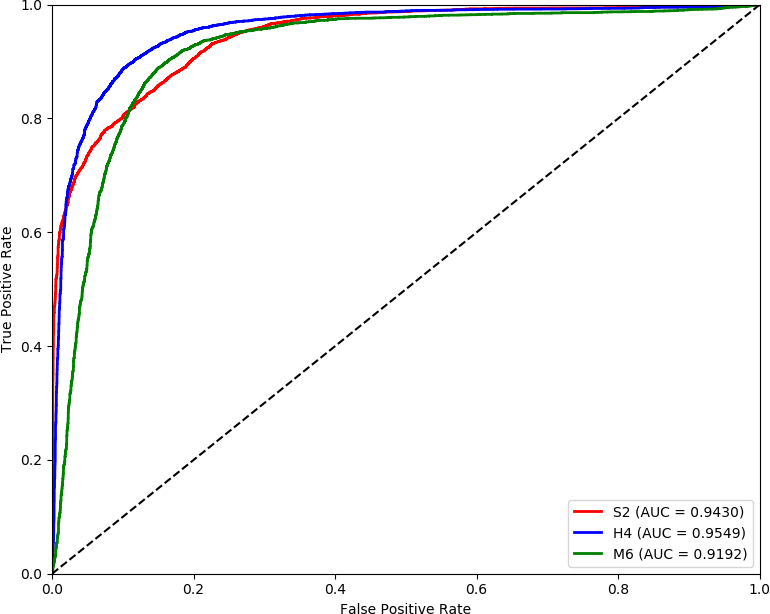
\includegraphics[width=.8\textwidth]{dados/figuras/ROC_H_10_6.png}
 \caption{Curvas ROC dos testes com o cenário H.10.6 para as CNNs treinadas com os conjuntos S2, H4 e M6 (Autoria própria).}
 \label{fig:I_Wanna_ROC!}
\end{figure}

Essa disparidade entre as métricas avaliadas pode ser explicada ao se analisar as matrizes de confusão\footnote{Matriz de confusão é uma tabela que mostra os resultados obtidos por um classificador. As linhas representam os rótulos reais, e as colunas o predito pelo classificador.} dos testes. A Tabela \ref{tab:matrix_reloaded} compara as matrizes de confusão, acurácia, precisão\footnote{Proporção de verdadeiros positivos em relação a todas predições positivas.} e revocação\footnote{Taxa de verdadeiros positivos.} obtidas pelas CNNs treinadas com os conjuntos S2 e H4 quando testados no cenário H.10.6.

\begin{table}[!htb]
\centering
\begin{tabular}{c|c|c|c|c|@{}m{0pt}@{}}
\cline{2-5}
		                          & \textbf{\begin{tabular}[c]{@{}c@{}}Matriz de\\ Confusão\end{tabular}}   & \textbf{Acurácia} & \textbf{Precisão} & \textbf{Revocação} &\\[20pt] \hline
\multicolumn{1}{|c|}{\textbf{H4}} & $\left[ \begin{array}{cc} 4156 & 844 \\ 300 & 4700 \end{array} \right]$ & 88,56\%           & 0.8477            & 0.94               &\\[21pt] \hline
\multicolumn{1}{|c|}{\textbf{S2}} & $\left[ \begin{array}{cc} 2548 & 2452 \\ 62 & 4938 \end{array} \right]$ & 74,86\%           & 0.6682            & 0.9876             &\\[21pt] \hline
\end{tabular}
\caption{Outras métricas dos testes realizados no cenário H.10.6 com as CNNs treinadas com os conjuntos H4 e S2.}
\label{tab:matrix_reloaded}
\end{table}

Também é interessante notar a baixa variação das acurácias para o \textit{payload} de 0.6 bpp, onde se tem um desvio padrão de apenas 0,093. A Tabela \ref{tab:cnn_s2} ilustra os resultados obtidos ao utilizar diferentes cenários de teste.

\begin{table}[!ht]
\centering
\begin{tabular}{c|c|c|c|c|}
\cline{2-5}
\textbf{}                             & \textbf{x = 0.1} & \textbf{x = 0.2} & \textbf{x = 0.4} & \textbf{x = 0.6} \\ \hline
\multicolumn{1}{|c|}{\textbf{H.0.x}}  & 56,1\%           & 67,59\%          & 73,59\%          & 74,76\%          \\ \hline
\multicolumn{1}{|c|}{\textbf{H.10.x}} & \textbf{57,94\%} & \textbf{69,02\%} & \textbf{73,87\%} & \textbf{74,86\%} \\ \hline
\multicolumn{1}{|c|}{\textbf{S.0.x}}  & 53,65\%          & 63,21\%          & 73,09\%          & 74,73\%          \\ \hline
\multicolumn{1}{|c|}{\textbf{S.7.x}}  & 55,03\%          & 66,78\%          & 73,65\%          & 74,83\%          \\ \hline
\multicolumn{1}{|c|}{\textbf{S.10.x}} & 54,69\%          & 65,59\%          & 73,47\%          & 74,76\%          \\ \hline
\multicolumn{1}{|c|}{\textbf{S.12.x}} & 54,3\%           & 65,36\%          & 73,45\%          & 74,79\%          \\ \hline
\multicolumn{1}{|c|}{\textbf{M.-.x}}  & 54,18\%          & 64,17\%          & 72,88\%          & 74,55\%          \\ \hline
\end{tabular}
\caption{Acurácias dos testes da CNN com o conjunto de treinamento S2.}
\label{tab:cnn_s2}
\end{table}

\subsection{Conjunto de Treinamento S4}

Os testes com a CNN treinada neste conjunto apresentaram bons resultados, ficando entre os melhores para \textit{payloads} de 0.1, 0.2 e 0.4 bpp para todos algoritmos. A Tabela \ref{tab:cnn_s4} apresenta as acurácias para todos os cenários de teste.

\begin{table}[!htb]
\centering
\begin{tabular}{c|c|c|c|c|}
\cline{2-5}
\textbf{}                             & \textbf{x = 0.1} & \textbf{x = 0.2} & \textbf{x = 0.4} & \textbf{x = 0.6} \\ \hline
\multicolumn{1}{|c|}{\textbf{H.0.x}}  & 53,78\%          & 66,74\%          & 80,25\%          & 84,43\%          \\ \hline
\multicolumn{1}{|c|}{\textbf{H.10.x}} & \textbf{55,21\%} & \textbf{69,04\%} & \textbf{81,07\%} & 84,50\%          \\ \hline
\multicolumn{1}{|c|}{\textbf{S.0.x}}  & 52,28\%          & 59,95\%          & 79,15\%          & 84,56\%          \\ \hline
\multicolumn{1}{|c|}{\textbf{S.7.x}}  & 53,08\%          & 64,30\%          & 80,94\%          & \textbf{84,89\%} \\ \hline
\multicolumn{1}{|c|}{\textbf{S.10.x}} & 52,82\%          & 62,80\%          & 80,43\%          & 84,77\%          \\ \hline
\multicolumn{1}{|c|}{\textbf{S.12.x}} & 52,64\%          & 62,39\%          & 80,00\%          & 84,65\%          \\ \hline
\multicolumn{1}{|c|}{\textbf{M.-.x}}  & 52,58\%          & 61,82\%          & 78,03\%          & 83,30\%          \\ \hline
\end{tabular}
\caption{Acurácias dos testes da CNN com o conjunto de treinamento S4.}
\label{tab:cnn_s4}
\end{table}


\subsection{Conjunto de Treinamento S6}

Este foi o conjunto de treinamento que obteve a maior acurácia para todos os cenários de teste do algoritmo S-UNIWARD com \textit{payload} de 0.6 bpp. Tendo mostrado também boa acurácia para outros algoritmos com o mesmo \textit{payload}. Porém foi um dos piores nos testes com \textit{payload} de 0.1 bpp, como pode ser visto na Tabela \ref{tab:cnn_s6}.

\begin{table}[!htb]
\centering
\begin{tabular}{c|c|c|c|c|}
\cline{2-5}
\textbf{}                             & \textbf{x = 0.1} & \textbf{x = 0.2} & \textbf{x = 0.4} & \textbf{x = 0.6} \\ \hline
\multicolumn{1}{|c|}{\textbf{H.0.x}}  & 51,12\%          & 59,21\%          & 75,72\%          & 87,01\%          \\ \hline
\multicolumn{1}{|c|}{\textbf{H.10.x}} & \textbf{51,67\%} & \textbf{61,38\%} & 77,58\%          & 87,86\%          \\ \hline
\multicolumn{1}{|c|}{\textbf{S.0.x}}  & 50,68\%          & 55,24\%          & 74,52\%          & 87,24\%          \\ \hline
\multicolumn{1}{|c|}{\textbf{S.7.x}}  & 50,98\%          & 58,51\%          & \textbf{77,67\%} & \textbf{89,12\%} \\ \hline
\multicolumn{1}{|c|}{\textbf{S.10.x}} & 50,72\%          & 57,16\%          & 76,50\%          & 88,37\%          \\ \hline
\multicolumn{1}{|c|}{\textbf{S.12.x}} & 50,81\%          & 56,80\%          & 75,89\%          & 88,12\%          \\ \hline
\multicolumn{1}{|c|}{\textbf{M.-.x}}  & 50,73\%          & 55,52\%          & 72,75\%          & 83,85\%          \\ \hline
\end{tabular}
\caption{Acurácias dos testes da CNN com o conjunto de treinamento S6.}
\label{tab:cnn_s6}
\end{table}


\subsection{Conjunto de Treinamento M1}

Este conjunto, treinado com a base contendo imagens esteganografadas com o algoritmo MiPOD, apresentou resultados medianos em todos os testes. A Tabela \ref{tab:cnn_m1} exibe as acurácias obtidas.

\begin{table}[!htb]
\centering
\begin{tabular}{c|c|c|c|c|}
\cline{2-5}
\textbf{}                             & \textbf{x = 0.1} & \textbf{x = 0.2} & \textbf{x = 0.4} & \textbf{x = 0.6} \\ \hline
\multicolumn{1}{|c|}{\textbf{H.0.x}}  & 52,87\%          & 61,84\%          & 77,76\%          & 83,15\%          \\ \hline
\multicolumn{1}{|c|}{\textbf{H.10.x}} & \textbf{53,80\%} & \textbf{64,64\%} & \textbf{79,00\%} & \textbf{83,56\%} \\ \hline
\multicolumn{1}{|c|}{\textbf{S.0.x}}  & 51,40\%          & 55,88\%          & 74,84\%          & 82,09\%          \\ \hline
\multicolumn{1}{|c|}{\textbf{S.7.x}}  & 51,98\%          & 58,11\%          & 77,29\%          & 83,08\%          \\ \hline
\multicolumn{1}{|c|}{\textbf{S.10.x}} & 51,72\%          & 57,42\%          & 76,28\%          & 82,85\%          \\ \hline
\multicolumn{1}{|c|}{\textbf{S.12.x}} & 51,65\%          & 57,07\%          & 76,02\%          & 82,63\%          \\ \hline
\multicolumn{1}{|c|}{\textbf{M.-.x}}  & 51,98\%          & 58,18\%          & 76,14\%          & 82,20\%          \\ \hline
\end{tabular}
\caption{Acurácias dos testes da CNN com o conjunto de treinamento M1.}
\label{tab:cnn_m1}
\end{table}

\subsection{Conjunto de Treinamento M2}

Assim como o conjunto S4, o M2 também ficou entre os melhores nos testes com \textit{payloads} de 0.1, 0.2, e 0.4 bpp, porém foi um dos piores nos testes com 0.6. A Tabela \ref{tab:cnn_m2} apresenta os resultados obtidos. Assim como na maioria dos testes, cenário H.10.x foi o que apresentou as maiores taxas de acurácia. 

\begin{table}[!htb]
\centering
\begin{tabular}{c|c|c|c|c|}
\cline{2-5}
\textbf{}                             & \textbf{x = 0.1} & \textbf{x = 0.2} & \textbf{x = 0.4} & \textbf{x = 0.6} \\ \hline
\multicolumn{1}{|c|}{\textbf{H.0.x}}  & 53,80\%          & 63,09\%          & 78,96\%          & 82,46\%          \\ \hline
\multicolumn{1}{|c|}{\textbf{H.10.x}} & \textbf{54,94\%} & \textbf{65,94\%} & \textbf{79,93\%} & \textbf{82,59\%} \\ \hline
\multicolumn{1}{|c|}{\textbf{S.0.x}}  & 52,25\%          & 57,86\%          & 75,74\%          & 81,92\%          \\ \hline
\multicolumn{1}{|c|}{\textbf{S.7.x}}  & 52,92\%          & 60,29\%          & 78,40\%          & 82,46\%          \\ \hline
\multicolumn{1}{|c|}{\textbf{S.10.x}} & 52,72\%          & 59,49\%          & 77,58\%          & 82,27\%          \\ \hline
\multicolumn{1}{|c|}{\textbf{S.12.x}} & 52,64\%          & 58,94\%          & 76,90\%          & 82,10\%          \\ \hline
\multicolumn{1}{|c|}{\textbf{M.-.x}}  & 52,94\%          & 60,59\%          & 77,46\%          & 82,00\%          \\ \hline
\end{tabular}
\caption{Acurácias dos testes da CNN com o conjunto de treinamento M2.}
\label{tab:cnn_m2}
\end{table}


\subsection{Conjunto de Treinamento M4}

A Tabela \ref{tab:cnn_m4} apresenta os resultados obtidos com este conjunto de treinamento, que teve boas taxas de acerto nos testes com \textit{payloads} de 0.4 e 0.6 bpp. Foi o melhor desempenho obtido em todos os testes para o cenário M.-.6, onde alcançou 85.94\% de acurácia, superando inclusive a abordagem com SRM + \textit{ensemble of classifiers}.

\begin{table}[!htb]
\centering
\begin{tabular}{c|c|c|c|c|}
\cline{2-5}
\textbf{}                             & \textbf{x = 0.1} & \textbf{x = 0.2} & \textbf{x = 0.4} & \textbf{x = 0.6} \\ \hline
\multicolumn{1}{|c|}{\textbf{H.0.x}}  & 51,61\%          & 57,49\%          & 79,67\%          & 86,44\%          \\ \hline
\multicolumn{1}{|c|}{\textbf{H.10.x}} & \textbf{52,17\%} & \textbf{60,59\%} & \textbf{81,55\%} & \textbf{87,05\%} \\ \hline
\multicolumn{1}{|c|}{\textbf{S.0.x}}  & 51,09\%          & 54,10\%          & 73,14\%          & 85,51\%          \\ \hline
\multicolumn{1}{|c|}{\textbf{S.7.x}}  & 51,36\%          & 55,54\%          & 78,52\%          & 86,48\%          \\ \hline
\multicolumn{1}{|c|}{\textbf{S.10.x}} & 51,28\%          & 54,83\%          & 76,12\%          & 86,25\%          \\ \hline
\multicolumn{1}{|c|}{\textbf{S.12.x}} & 51,24\%          & 54,73\%          & 75,43\%          & 86,08\%          \\ \hline
\multicolumn{1}{|c|}{\textbf{M.-.x}}  & 51,57\%          & 55,77\%          & 77,14\%          & 85,94\%          \\ \hline
\end{tabular}
\caption{Acurácias dos testes da CNN com o conjunto de treinamento M4.}
\label{tab:cnn_m4}
\end{table}

Observe que o desempenho para os \textit{payloads} 0.1 e 0.2 não foi bom, indicando que o treinamento para o \textit{payload} 0.4 deixa o classificador mais habilitado para identificar maiores quantidades de mensagens escondidas. Ao passo que o treinamento realizado com M1 e M2 obtém 64,64\% e 65,94\% de acurácia para o teste com \textit{payload }0.2, respectivamente, para o M4 o valor é de 60,59\%.

\subsection{Conjunto de Treinamento M6}

Os resultados do conjunto M6, mostrados na Tabela \ref{tab:cnn_m6}, foram os piores em comparação com os obtidos pelos outros conjuntos em grande parte dos testes. Apresentando resultados satisfatórios apenas quando testado com \textit{payload} de 0.6 bpp.

\begin{table}[!htb]
\centering
\begin{tabular}{c|c|c|c|c|}
\cline{2-5}
\textbf{}                             & \textbf{x = 0.1} & \textbf{x = 0.2} & \textbf{x = 0.4} & \textbf{x = 0.6} \\ \hline
\multicolumn{1}{|c|}{\textbf{H.0.x}}  & 50,52\%          & 51,86\%          & 65,65\%          & 84,16\%          \\ \hline
\multicolumn{1}{|c|}{\textbf{H.10.x}} & \textbf{50,63\%} & \textbf{52,29\%} & \textbf{69,96\%} & \textbf{86,12\%} \\ \hline
\multicolumn{1}{|c|}{\textbf{S.0.x}}  & 50,37\%          & 51,35\%          & 57,59\%          & 80,20\%          \\ \hline
\multicolumn{1}{|c|}{\textbf{S.7.x}}  & 50,45\%          & 51,63\%          & 61,46\%          & 84,46\%          \\ \hline
\multicolumn{1}{|c|}{\textbf{S.10.x}} & 50,44\%          & 51,59\%          & 59,65\%          & 82,80\%          \\ \hline
\multicolumn{1}{|c|}{\textbf{S.12.x}} & 50,39\%          & 51,60\%          & 59,30\%          & 82,28\%          \\ \hline
\multicolumn{1}{|c|}{\textbf{M.-.x}}  & 50,48\%          & 51,48\%          & 63,61\%          & 83,87\%          \\ \hline
\end{tabular}
\caption{Acurácias dos testes da CNN com o conjunto de treinamento M6.}
\label{tab:cnn_m6}
\end{table}


% \section{Detecção do LSB \textit{Matching}}
% 
% EXPLICAR AQUI PQ FOI USADA (PARA VALIDAÇÃO).
% MENCIONAR ESTADO DA ARTE (SE É VALIDAÇÃO, DEVE ESTAR COMPATÍVEL)!!!
% 
% O LSB-Matching~\citeauthorlsb_matching_revised} foi implementado em C++ pelos próprios autores desse trabalho segundo as especificações de \citeonline{sharp2001implementation} e \citeonline{lsb_matching_revised}\footnote{Disponível em: \url{https://github.com/yudi-matsuzake/stegim}.}. 
% 
% A Tabela \ref{tab:lsbespecial} mostra os resultados obtidos com cada um dos conjuntos de treinamento, quando testados com o LSB \textit{Matching}. Os resultados, 
%ESSA ARGUMENTAÇÃO NÃO ESTÁ BOA, CONFORME CONVERSAMOS!!!
%apesar de estarem não estado da arte de detecção do LSB \textit{Matching}, porém, nesse caso ele foi utilizado para apenas a validação da rede. Conforme exemplificado na Figura~\ref{fig:comp}, fica claro perceber o motivo desses resultados quando se analisa a diferença de abordagens dos algoritmos adaptativos e não-adaptativos.

% \begin{table}[!htb]
% \centering
% \caption{Acurácias da detecção do LSB \textit{Matching}.}
% \label{tab:lsbespecial}
% \begin{tabular}{c|c|c|c|c|}
% \cline{2-5}
%                                   & \textbf{0.1} & \textbf{0.2} & \textbf{0.4} & \textbf{0.6} \\ \hline
% \multicolumn{1}{|c|}{\textbf{H1}} & 53,93\%        & 65,03\%        & 83,34\%        & 86,86\%        \\ \hline
% \multicolumn{1}{|c|}{\textbf{H2}} & 53,21\%        & 63,47\%        & 86,62\%        & 89,77\%        \\ \hline
% \multicolumn{1}{|c|}{\textbf{H4}} & 54,25\%        & 70,75\%        & 89,94\%        & 91,06\%        \\ \hline
% \multicolumn{1}{|c|}{\textbf{H6}} & 52,79\%        & 68,85\%        & 91,67\%        & \textbf{95,22}\%        \\ \hline
% \multicolumn{1}{|c|}{\textbf{S1}} & 53,67\%        & 66,29\%        & 89,04\%        & 90,64\%        \\ \hline
% \multicolumn{1}{|c|}{\textbf{S2}} & \textbf{60,81}\%        & 73,75\%        & 75,19\%        & 75,37\%        \\ \hline
% \multicolumn{1}{|c|}{\textbf{S4}} & 60,51\%        & \textbf{81,84}\%        & 86,02\%        & 86,3 \%        \\ \hline
% \multicolumn{1}{|c|}{\textbf{S6}} & 57,75\%        & 79,86\%        & \textbf{93,15}\%        & 93,97\%        \\ \hline
% \multicolumn{1}{|c|}{\textbf{M1}} & 55,41\%        & 72,89\%        & 84,38\%        & 85,71\%        \\ \hline
% \multicolumn{1}{|c|}{\textbf{M2}} & 55,88\%        & 73,42\%        & 84,26\%        & 84,91\%        \\ \hline
% \multicolumn{1}{|c|}{\textbf{M4}} & 53,99\%        & 68,46\%        & 87,99\%        & 89,06\%        \\ \hline
% \multicolumn{1}{|c|}{\textbf{M6}} & 51,78\%        & 57,68\%        & 86,62\%        & 92,26\%        \\ \hline
% \end{tabular}
% \end{table}

\section{Análise dos Resultados}

Os experimentos realizados com o uso de SRM e \textit{ensemble} de classificadores revelaram que essa abordagem é inadequada para esteganálise cega, isto é, detectar a presença de uma mensagem oculta sem conhecimento prévio do algoritmo e \textit{payload} utilizados. Os resultados obtidos só foram bons quando o treinamento e teste foi feito com o mesmo algoritmo, e com uma taxa de bits por pixel igual ou parecida.

Já a CNN, apesar de não ter alcançado os mesmos valores de acurácia que o \textit{ensemble} de classificadores em esteganálise direcionada, se mostrou muito mais eficaz para esteganálise cega, especialmente quando treinada com \textit{payloads} de 0.2 e 0.4 bpp. As únicas exceções a isso são as CNNs treinadas com MiPOD e S-UNIWARD com 0.2 bpp quando testadas com \textit{payload} de 0.6 bpp, onde a acurácia obtida foi muito baixa.

Uma das primeiras hipóteses consideradas no início desse trabalho era que os kernels da CNN poderiam se aproximar dos filtros SRM. Porém, isso não pode ser confirmado com os experimentos,  uma vez que os dois detectores se comportam de forma diferente --- a CNN tendo poder de generalização maior enquanto o SRM se mostra mais especializado.

Outro comportamento pertinente ao se usar a CNN foi a obtenção de piores resultados ao se usar os \textit{payloads} de 0.1 bpp e 0.6 bpp para o treinamento. Isso provavelmente ocorre porque quanto mais extremo o \textit{payload}, mais especializada tende a ficar a rede.

É possível notar também que, nos cenários onde foi utilizado o STC, a acurácia dos detectores foi maior, tanto do SRM e \textit{ensemble} de classificadores quanto da CNN.

Como já esperado, o algoritmo com o uso do descritor SRM teve desempenho notável quando se testando com o algoritmo HUGO, principalmente pelo fato de ter sido estruturado para a esteganálise do mesmo. O que acabou sendo surpreendente é que o seu melhor desempenho é muito superior ao da CNN, diferença discrepante com relação ao resultados dos outros algoritmos. Como pode ser observado na Tabela \ref{tab:hugo_comp}, nos cenários H.0.1 e H.10.1  a diferença chegou a um máximo de 10\%.

\begin{table}[h]
\centering
\caption{Comparação entre os melhores resultados para o algoritmo HUGO com uso do SRM e com uso da CNN}
\label{tab:hugo_comp}
\begin{tabular}{|c|c|c|c|c|c|c|c|c|}
\hline
    & H.0.1   & H.0.2   & H.0.4   & H.0.6   & H.10.1  & H.10.2  & H.10.4  & H.10.6  \\ \hline
SRM & 66,23\% & 73,89\% & 84,60\% & 90,46\% & 67,02\% & 75,30\% & 85,43\% & 91,18\% \\ \hline
CNN & 56,10\% & 67,59\% & 80,25\% & 88,01\% & 57,94\% & 69,04\% & 81,55\% & 88,56\% \\ \hline
\end{tabular}
\end{table}

Apesar das acurácias diferirem bastante, principalmente para o algoritmo HUGO, as AUCs para o \textit{payload} de 0.1 bpp não tem um contraste tão evidente, como mostrado na Figura \ref{fig:ROC_H}(a), na qual a CNN chegou, inclusive, a ter a curva superior ao SRM em vários pontos. Esse mesmo comportamento não se repete para o \textit{payload} de 0.6 bpp, como pode ser visto na Figura \ref{fig:ROC_H}(b), onde a curva do SRM é sempre superior a da CNN.

\begin{figure}[!ht]
\centering
	\subfloat[HUGO 0.1]{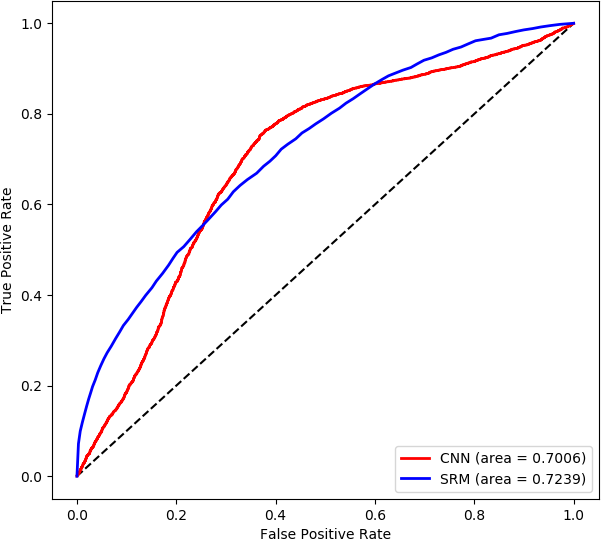
\includegraphics[width=0.45\textwidth]{dados/figuras/H1_H_0_1.png}}\;
	\subfloat[HUGO 0.6]{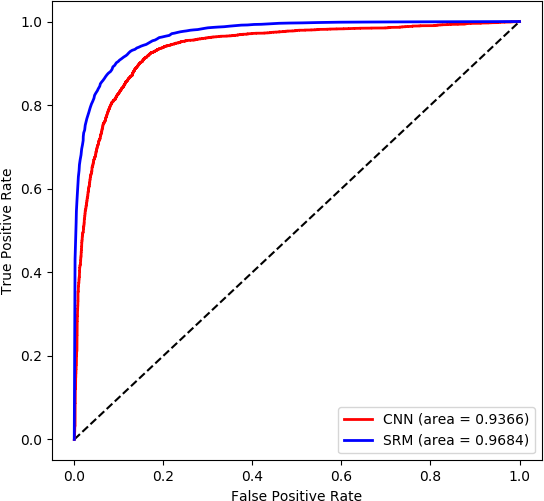
\includegraphics[width=0.45\textwidth]{dados/figuras/H6_H_0_6.png}} 
	\caption{Curvas ROC da CNN e do SRM para os cenários de teste e treino iguais (Autoria própria)}
    \label{fig:ROC_H}
\end{figure}

A Figura \ref{fig:ROC_M} ilustra um conjunto de treino no qual o SRM teve desempenho inferior à CNN em todos os cenários de teste que fazem uso do MiPOD, tanto com relação as acurácias quanto as AUCs. Isso ocorre porque o treino foi feito com um algoritmo de menor complexidade que o de teste, situação que piora consideravelmente a performance do SRM.

\begin{figure}[!htb]
 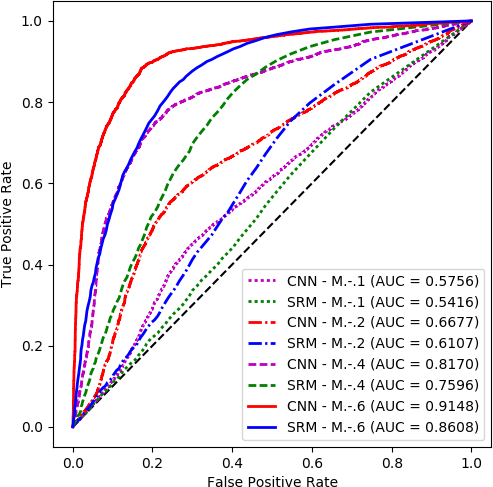
\includegraphics[width=.8\textwidth]{dados/figuras/H6_M-_x.png}
 \caption{Curvas ROC dos testes com o MiPOD e treinos com o cenário H6. (Autoria própria).}
 \label{fig:ROC_M}
\end{figure}

Uma característica em comum às duas arquiteturas foi a maior dificuldade de detectar a presença do algoritmo MiPOD. No caso do SRM, isso é ainda mais notável quando o classificador é treinado com um algoritmo diferente do MiPOD.

Com relação ao desempenho computacional, foi possível notar que o tempo de treino do \textit{ensemble} de classificadores com FLD é muito menor que o da CNN, porém o descritor SRM tem alta complexidade computacional pela quantidade de convoluções que são realizadas para cada filtro do algoritmo. Mesmo com a alta complexidade do descritor, a CNN é mais custosa computacionalmente no processo como um todo. 

Os Apêndices~\ref{chap:apendiceA} e \ref{chap:apendiceB} apresentam os valores de AUC para as duas abordagens.

                    % Resultados
% \include{estrutura/textuais/desenvolvimento/orientacoes}                   % Capítulo com Orientações de uso do Template
% % CONCLUSÃO--------------------------------------------------------------------

\chapter{Conclusão}
\label{chap:conclusao}

Uma das contribuições importantes do trabalho é ser uma literatura moderna sobre esteganografia e esteganálise, visto que há certa defasagem desses assuntos na literatura em português. Esses temas tem ganhado notoriedade na comunidade científica e são áreas de estudo complexas e multidisciplinares que tocam, por exemplo, as áreas de Processamento de Sinais, Segurança da Informação, Teoria da Informação e Teoria dos Códigos. Além disso, também foi utilizada uma abordagem de esteganálise com \textit{deep learning} que é um dos métodos que estão sendo investigados atualmente por estegoanalistas.

Nos resultados, a utilização dos descritores SRM em	 um \textit{ensemble} de classificadores FLD obteve resultados melhores quando o treinamento e teste foram feitos no mesmo cenário, ou seja, quando o classificador foi treinado e testado em estego imagens geradas pelo mesmo algoritmo de esteganografia e com o mesmo \textit{payload}. 

A CNN se comportou de maneira distinta, tendo resultados semelhantes mesmo quando testada em cenários diferentes. Ela generaliza os casos de teste de tal forma que funciona similarmente em diversos cenários, enquanto a abordagem utilizando SRM é mais especializada e funciona melhor para um cenário. 

Estes resultados sugerem que a CNN é mais apropriada para a utilização em ambientes de esteganálise cega e o \textit{ensemble} de classificadores se comporta  melhor em ambientes de esteganálise direcionada. Essa diferença de resultados também indica que a CNN não está aprendendo algo semelhante aos filtros do SRM.

Essas observações acerca da natureza das duas abordagens foi possível devido a uma metodologia onde, para cada conjunto de treinamento (que consideraram a combinação de diferentes algoritmos de esteganografia e \textit{payloads}), foram utilizados dois classificadores: CNN e \textit{ensemble} de classificadores (FLD como base). Eles foram aplicados para classificar diversos cenários de teste gerados nesse trabalho. Assim, podemos analisar a diferença das duas abordagens em diversos contextos de esteganálise.

Abordagens de \textit{deep learning} estão sendo aplicadas com sucesso em diversos problemas difíceis de Processamento de Sinais. Em esteganálise não é diferente, com bons resultados recentes utilizando CNNs \citeauthor{tan2014stacked,qian2015deep,cnn_base,xu2016ensemble}. Portanto, o estudo de esteganálise com CNN é bastante promissor, ainda tendo lacunas de possíveis metodologias, arquiteturas e camadas relacionadas a otimização da rede especificamente para problemas de esteganálise há serem exploradas.

\section{Trabalhos Futuros}
\label{sec:trabalhosFuturos}

Os resultados desse trabalho mostraram as diferenças de generalização e especificação dos detectores de esteganografia. Uma continuação desse trabalho, utilizando a mesma metodologia poderia ser a criação de um \textit{Ensamble of CNNs}, com o fim de aumentar a acurácia sem perder a generalização. Além dessa mudança da forma em que as CNNs são utilizadas, é possível também alterar a estrutura interna de cada uma das CNNs.

Há diferentes e novas estruturas de CNN que estão sendo investigadas para resolver diferentes problemas. Alguns exemplos são as \textit{Recurrent Neural Networks}, \textit{Residual Neural Networks}, \textit{Region Based CNN} entre outras. Essas arquiteturas podem ser exploradas com a finalidade de solucionar problemas de esteganálise, como o trabalho de \citeonline{wu2017deep} onde é utilizado uma \textit{Residual Neural Network} com $\approx 60$ camadas. Algumas dessas arquiteturas favorecem intuitivamente alguns problemas da esteganálise forense como, por exemplo, uma \textit{Region Based CNN} poderia ser treinada para descobrir a localização dos dados embutidos e, com isso, obter dicas do algoritmo que foi utilizado. \textit{Recurrent Neural Networks} criam relações entre as camadas o que poderia ser utilizado para a estimativa de \textit{payloads}.

Como o SRM para esteganálise direcionada obteve mais sucesso nos testes realizados, os kernels da CNN poderiam ser inicializados com os filtros lineares desse descritor (o que seria uma forma de explorar o comportamento desses detectores). Também, trabalhos como os de \citeonline{denemark2014selection} e \citeonline{denemark2016improving} buscam aprimoramentos, alterações e acréscimos nos descritores SRM. Esses trabalhos podem também ser explorados em conjunto com CNNs.

\citeonline{sedighi2016content} apresentaram uma definição rigorosa de modelos de imagens de cobertura e estego imagens, conseguindo chegar em uma fórmula fechada para um detector ótimo de esteganografia % (essa fórmula pode ser vista na Equação~\ref{eq:deteccao-otima}) 
que elevou o compreendimento sobre os limites da esteganálise. Esses resultados podem ser utilizados para a criação de novos métodos e arquiteturas de CNNs para esteganálise.

Recentemente, \citeonline{sedighi2017histogram} publicaram resultados sobre a implementação de uma nova camada para CNN chamada de \textit{Histogram Layer}, criada especificamente para melhorar resultados em esteganálise. Apesar do estado da arte não ser atingido, esses resultados foram importantes como prova de conceito de uma rede com informações e métodos esteganográficos previamente conhecidos, deixando a dúvida da existência de outros métodos similares misturando conhecimentos de esteganálise com aprendizado das CNNs.

% \section{CONSIDERAÇÕES FINAIS}
% \label{sec:consideracoesFinais}

%A escalabilidade com o número de amostras para treino sem perda de performance na classificação, se igualando a classificadores bem estabelecidos, com SVM, em conjunto com as outras características já listadas tornam o \textit{Ensemble of Classifiers} de FLDs ideal para o experimento proposto.%, no qual é aplicado um descritor de alta dimensionalidade (SRM) a uma grande quantidade de imagens para treino.
                 			   % Conclusão
% \include{estrutura/textuais/desenvolvimento/viabilidade-cronograma}

\postextual
% INSERE ELEMENTOS PÓS-TEXTUAIS
% REFERÊNCIAS------------------------------------------------------------------

% Carrega o arquivo "base-referencias.bib" e extrai automaticamente as referências citadas

\bibliography{./base-referencias}
\bibliographystyle{abntex2-num} % Define o estilo ABNT para formatar a lista de referências
% OBSERVAÇÕES------------------------------------------------------------------
% Este arquivo não precisa ser alterado.
           			   % Referências
% % APÊNDICES--------------------------------------------------------------------

\begin{apendicesenv}
\partapendices

% Primeiro apêndice------------------------------------------------------------
\chapter{Tabela de AUCs do SRM} % Edite para alterar o título deste apêndice
\label{chap:apendiceA}

\begin{table}[!ht]
\centering
\caption{AUCs do \textit{Ensemble of Classifiers} treinado com o descritor SRM para o algoritmo HUGO}
\label{tab:auc_hugo}
\begin{tabular}{|c|c|c|c|c|}
\hline
                & \textbf{H1} & \textbf{H2} & \textbf{H4} & \textbf{H6} \\ \hline
\textbf{H.0.1}  & 0,7337      & 0,7075      & 0,6396      & 0,6034      \\ \hline
\textbf{H.10.1} & 0,7470      & 0,7269      & 0,6596      & 0,6192      \\ \hline
\textbf{H.0.2}  & 0,8329      & 0,8352      & 0,7935      & 0,7525      \\ \hline
\textbf{H.10.2} & 0,8444      & 0,8483      & 0,8122      & 0,7718      \\ \hline
\textbf{H.0.4}  & 0,9181      & 0,9322      & 0,9291      & 0,9147      \\ \hline
\textbf{H.10.4} & 0,9243      & 0,8391      & 0,9384      & 0,9273      \\ \hline
\textbf{H.0.6}  & 0,9528      & 0,9660      & 0,9712      & 0,9693      \\ \hline
\textbf{H.10.6} & 0,9561      & 0,9690      & 0,9743      & 0,9736      \\ \hline
\textbf{S.0.1}  & 0,6305      & 0,5847      & 0,5519      & 0,5388      \\ \hline
\textbf{S.10.1} & 0,6451      & 0,6014      & 0,5629      & 0,5481      \\ \hline
\textbf{S.0.2}  & 0,7469      & 0,7160      & 0,6528      & 0,6237      \\ \hline
\textbf{S.0.4}  & 0,8653      & 0,8673      & 0,8349      & 0,7967      \\ \hline
\textbf{S.10.4} & 0,8749      & 0,8801      & 0,8524      & 0,8158      \\ \hline
\textbf{S.0.6}  & 0,9259      & 0,9347      & 0,9268      & 0,8995      \\ \hline
\textbf{M.0.1}  & 0,6212      & 0,5800      & 0,5476      & 0,5363      \\ \hline
\textbf{M.0.2}  & 0,7170      & 0,6893      & 0,6335      & 0,6061      \\ \hline
\textbf{M.0.4}  & 0,8230      & 0,8275      & 0,7962      & 0,7599      \\ \hline
\textbf{M.0.6}  & 0,8838      & 0,8998      & 0,8913      & 0,8651      \\ \hline
\end{tabular}
\end{table}




% Novo apêndice----------------------------------------------------------------
\chapter{Tabelas de AUCs da CNN}
\label{chap:apendiceB}

\begin{table}[!h]
\centering
\caption{AUCs das CNNs treinadas com HUGO}
\begin{tabular}{|c|c|c|c|c|}
\hline
\textbf{}       & \textbf{H1} & \textbf{H2} & \textbf{H4} & \textbf{H6} \\ \hline
\textbf{H.0.1}  & 0,6119      & 0,6162      & 0,6014      & 0,6029      \\ \hline
\textbf{H.10.1} & 0,6337      & 0,6402      & 0,6234      & 0,6200      \\ \hline
\textbf{H.0.2}  & 0,7006      & 0,7173      & 0,7179      & 0,7056      \\ \hline
\textbf{H.10.2} & 0,7273      & 0,7466      & 0,7473      & 0,7275      \\ \hline
\textbf{H.0.4}  & 0,8304      & 0,8621      & 0,8788      & 0,8542      \\ \hline
\textbf{H.10.4} & 0,8538      & 0,8837      & 0,8967      & 0,8727      \\ \hline
\textbf{H.0.6}  & 0,9085      & 0,9367      & 0,9478      & 0,9366      \\ \hline
\textbf{H.10.6} & 0,9207      & 0,9459      & 0,9549      & 0,9456      \\ \hline
\textbf{S.0.1}  & 0,5609      & 0,5589      & 0,5558      & 0,5648      \\ \hline
\textbf{S.7.1}  & 0,5758      & 0,5744      & 0,5705      & 0,5808      \\ \hline
\textbf{S.10.1} & 0,5717      & 0,5700      & 0,5667      & 0,5765      \\ \hline
\textbf{S.12.1} & 0,5692      & 0,5672      & 0,5636      & 0,5731      \\ \hline
\textbf{S.0.2}  & 0,6331      & 0,6372      & 0,6402      & 0,6560      \\ \hline
\textbf{S.7.2}  & 0,6554      & 0,6638      & 0,6706      & 0,6829      \\ \hline
\textbf{S.10.2} & 0,6480      & 0,6553      & 0,6604      & 0,6737      \\ \hline
\textbf{S.12.2} & 0,6449      & 0,6508      & 0,6559      & 0,6703      \\ \hline
\textbf{S.0.4}  & 0,7583      & 0,7926      & 0,8268      & 0,8183      \\ \hline
\textbf{S.7.4}  & 0,7850      & 0,8243      & 0,8580      & 0,8450      \\ \hline
\textbf{S.10.4} & 0,7751      & 0,8125      & 0,8470      & 0,8353      \\ \hline
\textbf{S.12.4} & 0,7698      & 0,8059      & 0,8402      & 0,8298      \\ \hline
\textbf{S.0.6}  & 0,8586      & 0,9043      & 0,9301      & 0,9194      \\ \hline
\textbf{S.7.6}  & 0,8820      & 0,9239      & 0,9436      & 0,9354      \\ \hline
\textbf{S.10.6} & 0,8728      & 0,9165      & 0,9388      & 0,9293      \\ \hline
\textbf{S.12.6} & 0,8694      & 0,9133      & 0,9360      & 0,9263      \\ \hline
\textbf{M.-.1}  & 0,5702      & 0,5690      & 0,5658      & 0,5756      \\ \hline
\textbf{M.-.2}  & 0,6487      & 0,6564      & 0,6601      & 0,6677      \\ \hline
\textbf{M.-.4}  & 0,7799      & 0,8128      & 0,8338      & 0,8170      \\ \hline
\textbf{M.-.6}  & 0,8759      & 0,9109      & 0,9251      & 0,9148      \\ \hline
\end{tabular}
\end{table}


\begin{table}[!htb]
\centering
\caption{AUCs das CNNs treinadas com S-UNIWARD}
\begin{tabular}{|c|c|c|c|c|}
\hline
\textbf{}       & \textbf{S1} & \textbf{S2} & \textbf{S4} & \textbf{S6} \\ \hline
\textbf{H.0.1}  & 0,5640      & 0,5854      & 0,6054      & 0,5793      \\ \hline
\textbf{H.10.1} & 0,5770      & 0,6023      & 0,6228      & 0,5941      \\ \hline
\textbf{H.0.2}  & 0,6421      & 0,7034      & 0,7148      & 0,6869      \\ \hline
\textbf{H.10.2} & 0,6629      & 0,7306      & 0,7346      & 0,7061      \\ \hline
\textbf{H.0.4}  & 0,7970      & 0,8759      & 0,8729      & 0,8428      \\ \hline
\textbf{H.10.4} & 0,8181      & 0,8900      & 0,8879      & 0,8573      \\ \hline
\textbf{H.0.6}  & 0,8875      & 0,9362      & 0,9489      & 0,9336      \\ \hline
\textbf{H.10.6} & 0,8964      & 0,9430      & 0,9543      & 0,9414      \\ \hline
\textbf{S.0.1}  & 0,5435      & 0,5593      & 0,5741      & 0,5549      \\ \hline
\textbf{S.7.1}  & 0,5534      & 0,5752      & 0,5930      & 0,5703      \\ \hline
\textbf{S.10.1} & 0,5503      & 0,5707      & 0,5877      & 0,5657      \\ \hline
\textbf{S.12.1} & 0,5488      & 0,5681      & 0,5843      & 0,5631      \\ \hline
\textbf{S.0.2}  & 0,6062      & 0,6552      & 0,6782      & 0,6552      \\ \hline
\textbf{S.7.2}  & 0,6273      & 0,6885      & 0,7055      & 0,6845      \\ \hline
\textbf{S.10.2} & 0,6203      & 0,6771      & 0,6964      & 0,6752      \\ \hline
\textbf{S.12.2} & 0,6174      & 0,6723      & 0,6931      & 0,6710      \\ \hline
\textbf{S.0.4}  & 0,7559      & 0,8528      & 0,8521      & 0,8322      \\ \hline
\textbf{S.7.4}  & 0,7904      & 0,8779      & 0,8810      & 0,8579      \\ \hline
\textbf{S.10.4} & 0,7778      & 0,8688      & 0,8697      & 0,8477      \\ \hline
\textbf{S.12.4} & 0,7711      & 0,8641      & 0,8643      & 0,8427      \\ \hline
\textbf{S.0.6}  & 0,8746      & 0,9290      & 0,9465      & 0,9344      \\ \hline
\textbf{S.7.6}  & 0,8904      & 0,9393      & 0,9561      & 0,9489      \\ \hline
\textbf{S.10.6} & 0,8852      & 0,9357      & 0,9526      & 0,9434      \\ \hline
\textbf{S.12.6} & 0,8820      & 0,9338      & 0,9507      & 0,9404      \\ \hline
\textbf{M.-.1}  & 0,5482      & 0,5653      & 0,5821      & 0,5617      \\ \hline
\textbf{M.-.2}  & 0,6141      & 0,6627      & 0,6830      & 0,6563      \\ \hline
\textbf{M.-.4}  & 0,7620      & 0,8504      & 0,8408      & 0,8117      \\ \hline
\textbf{M.-.6}  & 0,8686      & 0,9242      & 0,9326      & 0,9102      \\ \hline
\end{tabular}
\end{table}

\begin{table}[!htb]
\centering
\caption{AUCs das CNNs treinadas com MiPOD}
\begin{tabular}{|c|c|c|c|c|}
\hline
\textbf{}       & \textbf{M1} & \textbf{M2} & \textbf{M4} & \textbf{M6} \\ \hline
\textbf{H.0.1}  & 0,5828      & 0,5867      & 0,5741      & 0,5738      \\ \hline
\textbf{H.10.1} & 0,5980      & 0,6025      & 0,5896      & 0,5872      \\ \hline
\textbf{H.0.2}  & 0,6660      & 0,6774      & 0,6725      & 0,6610      \\ \hline
\textbf{H.10.2} & 0,6864      & 0,7010      & 0,7009      & 0,6823      \\ \hline
\textbf{H.0.4}  & 0,7927      & 0,8273      & 0,8557      & 0,8129      \\ \hline
\textbf{H.10.4} & 0,8129      & 0,8479      & 0,8767      & 0,8334      \\ \hline
\textbf{H.0.6}  & 0,8853      & 0,9183      & 0,9394      & 0,9062      \\ \hline
\textbf{H.10.6} & 0,9000      & 0,9298      & 0,9482      & 0,9192      \\ \hline
\textbf{S.0.1}  & 0,5537      & 0,5583      & 0,5493      & 0,5514      \\ \hline
\textbf{S.7.1}  & 0,5670      & 0,5723      & 0,5618      & 0,5642      \\ \hline
\textbf{S.10.1} & 0,5633      & 0,5683      & 0,5584      & 0,5607      \\ \hline
\textbf{S.12.1} & 0,5609      & 0,5661      & 0,5562      & 0,5587      \\ \hline
\textbf{S.0.2}  & 0,6240      & 0,6327      & 0,6231      & 0,6226      \\ \hline
\textbf{S.7.2}  & 0,6461      & 0,6566      & 0,6490      & 0,6459      \\ \hline
\textbf{S.10.2} & 0,6390      & 0,6489      & 0,6403      & 0,6384      \\ \hline
\textbf{S.12.2} & 0,6358      & 0,6451      & 0,6368      & 0,6353      \\ \hline
\textbf{S.0.4}  & 0,7521      & 0,7803      & 0,8053      & 0,7711      \\ \hline
\textbf{S.7.4}  & 0,7780      & 0,8098      & 0,8429      & 0,8011      \\ \hline
\textbf{S.10.4} & 0,7684      & 0,7986      & 0,8288      & 0,7898      \\ \hline
\textbf{S.12.4} & 0,7633      & 0,7930      & 0,8214      & 0,7838      \\ \hline
\textbf{S.0.6}  & 0,8513      & 0,8897      & 0,9236      & 0,8830      \\ \hline
\textbf{S.7.6}  & 0,8753      & 0,9116      & 0,9396      & 0,9045      \\ \hline
\textbf{S.10.6} & 0,8662      & 0,9035      & 0,9336      & 0,8968      \\ \hline
\textbf{S.12.6} & 0,8619      & 0,8992      & 0,9306      & 0,8922      \\ \hline
\textbf{M.-.1}  & 0,5674      & 0,5711      & 0,5619      & 0,5643      \\ \hline
\textbf{M.-.2}  & 0,6465      & 0,6562      & 0,6504      & 0,6468      \\ \hline
\textbf{M.-.4}  & 0,7763      & 0,8097      & 0,8378      & 0,8021      \\ \hline
\textbf{M.-.6}  & 0,8743      & 0,9094      & 0,9342      & 0,9042      \\ \hline
\end{tabular}
\end{table}


\end{apendicesenv}
             			   % Apêndices
% \include{estrutura/pos-textuais/anexos}               			   % Anexos

\end{document}
